
\section{Experiments}~
In the following, we compare Python implementations of our algorithms with baselines like simple Gibbs sampling, 
and particle MCMC sampling. Unless specified, our results were
obtained from $100$ independent MCMC runs, each consisting of $10000$ iterations.
We found particle MCMC to be more computationally intensive, and limited each 
run to $3000$ iterations, the number of particles being $5, 10$ and $20$. 
We also considered exploiting gradient information of the target distribution to 
apply Hamiltonian Monte Carlo (HMC)~\cite{Neal2010}. In particular, the forward 
pass of FFBS allows us to also calculate the gradient of the log-probability with
respect to the MJP parameters. We can exploit this information to explore parameter
space more efficiently than a random-walk algorithm. We run HMC with the number of leapfrog steps taking values in $1, 3, 5$ or $10$, and the leapfrog stepsize in 
$0.02, 0.05$ and $0.1$. 

For each run of each MCMC algorithm, we calculated the effective sample size (ESS) of the posterior samples of the MJP parameters using the R 
package \texttt{rcoda}~\cite{Rcoda2006}. This estimates the number of independent samples returned by the MCMC algorithm,
and dividing this by the runtime of a 
simulation gives the ESS per unit time. We used this as a measure to compare different Monte Carlo samplers and three different k's, $1.5, 2$ and $3$. Where $\Omega(\theta) = k \max A(\theta) $ for Naive MH sampler and Gibbs Sampler. For Exchange MH sampler, when $k = 1.5$,  $\Omega(\theta, \theta^*) = k \max(\max A(\theta), \max A(\theta^*))$. For $k=$ $2$ or $3$, $\Omega(\theta, \theta^*) = \frac{k}{2} (\max A(\theta) + \max A(\theta^*))$  \vinayak{What is k?}. 

% \begin{algorithm}[!ht]
%    \caption{Generic Gibbs sampling for MJPs for Gamma priors}
%    \label{alg:Generic Gibbs}
% \begin{algorithmic}
%    \State {\bfseries Input:} observations $y_{[t_0, t_{k+1})}$
%    \State Initialize, $i = 0$
%    \\ (a) Set $\alpha(0), \beta(0)$ arbitrarily and set current trajectory $[S,T](0)$ arbitrarily.\\
%     (b) Uniformize $[S,T](0)$, to get virtual jumps $U$.
%    \Repeat
%    \For{$i=1$ {\bfseries to} $N$}
%     \State (a) Sample $U(i) \sim P( U | \beta(i - 1), \alpha(i - 1), S(i - 1), T(i - 1), y)$.\\	
%     \State (b) Use FFBS algorithm to  sample states given all the jump times(both true jumps and virtual jumps).
% (i.e. $V(i) \sim P(V |  \beta(i - 1), \alpha(i - 1), W(i ), y).$) Then delete all the virtual jumps to get $S(i), T(i) .$\\
%     \State (c) Propose $\beta^* \sim q(.| \beta(i -1))$.\\
%       Set $\beta(i) = \beta^*$, with probability $P_{acc} = 1 \wedge \frac{P(\beta^* |S(i), T(i))}{P(\beta(i - 1) |S(i), T(i))} \frac{q(\beta(i - 1)|\beta^*)}{q(\beta^*|\beta(i - 1))}$;\\Otherwise set $\beta(i) = \beta(i-1)$.\\	  
%     \State (d) Sample $\alpha(i) \sim P(. | \beta(i), S(i), T(i), y)$.\\ It is a $Gamma(\mu + N, \lambda + \sum_{0}^NF_{S_i}(\beta)(t_{i + 1} - t_i))$ distribution actually.\\
%     \EndFor
%     \Until{$ i = N$ }
%  \end{algorithmic}
%  \end{algorithm}

\subsection{An MJP with exponentially decaying rates}
  \begin{figure}[H]
  \centering
  \begin{minipage}[!hp]{0.45\linewidth}
  \centering
    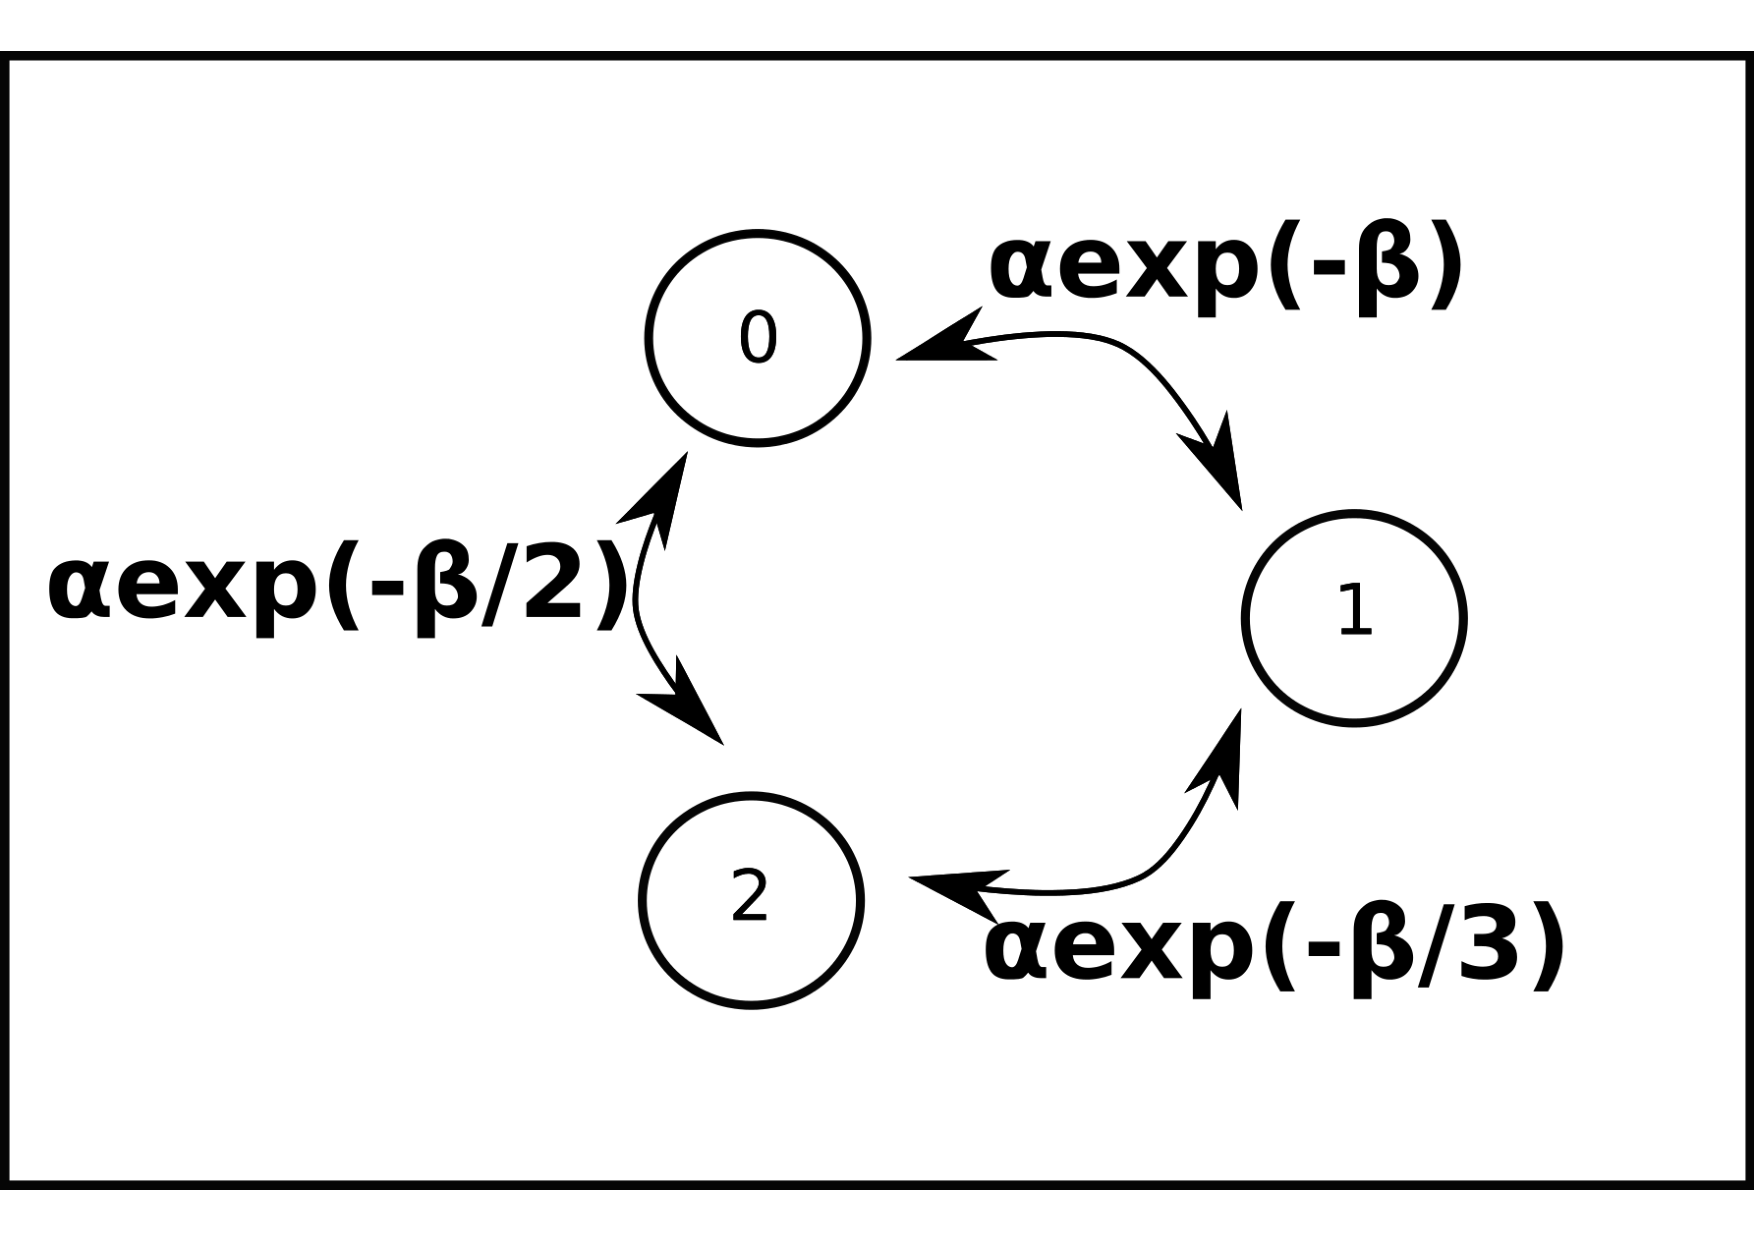
\includegraphics [width=0.70\textwidth, angle=0]{figs/exp_model.pdf}
      \end{minipage}
    \caption{A 3-state MJP with exponentially decaying rates}
    \label{fig:exp_model}
  \end{figure}

% \noindent Assume: $S = [S_0,S_1, ...,S_N] \;, T = [t_0(t_{start}), t_1,...,t_N, t_{N+1}(t_{end})]$, and y as observations.\\
% We consider a specific structure of rate matrix $A$. $A_{ij} = \alpha f_{ij}(\beta), \; i \neq j$. $A_{ii} = -\sum_{j \neq i} A_{ij}$. $0 \leq f_{ij} \leq 1$. Denote $F_i(\beta) = \sum_{j \neq i} f_{ij}(\beta)$.\\
% \begin{align*}
% P(s_0, S, T | \alpha, \beta) &= \pi_0(s_0)\prod_{i = 1}^N A_{S_{i - 1}S_i} \exp(- \int_{t_{start}}^{t_{end}} |A_{S(t)}| dt)\\
% &= \pi_0(s_0) \alpha^N \prod_{i = 1}^N f_{S_{i - 1}S_i} \exp(-\alpha  \sum_{i = 0}^{N} F_{S_i}(\beta)(t_{i + 1} - t_i))\\
% \end{align*} 
\noindent First consider a simple MJP with two parameters $\alpha$ and $\beta$, transitions between states $i$ and $j$ having rate $\alpha \exp(-\beta/(i+j))$.
We consider three settings for number of states, $3, 5$ and $10$.
Figure~\ref{fig:exp_model} shows the situation with $3$ states.  
We placed Gamma$(\alpha_0,\alpha_1)$, and Gamma$(\beta_0, \beta_1)$ priors on the parameters $\alpha$, $\beta$, with $(\alpha_0,\alpha_1,\beta_0,\beta_1)$ taking
values $(3,2,5,2)$ respectively. In our experiments, we used random parameters drawn from these prior distributions to construct a transition matrix $A$,
and placing a uniform distribution over states at time $0$, sampled an MJP trajectory.
Our observation process was a Gaussian distribution with mean equal to the current state and variance equal to $1$. There are $19$ observations uniformly observed between the time interval $[0, 20]$.
\vinayak{Number of observations?}

\vinayak{We studied our MH sampler, for three setting of $k$}.  For our proposal distribution, we used a lognormal distribution centered at the current
parameter value, and with a user-specified tuning parameter.
% %\begin{align*}
% %P(\alpha, \beta | s_0, S, T ) \propto \alpha^N \prod_{i = 1}^N f_{S_{i - 1}S_i} \exp(-\alpha  \sum_{i = 0}^{N} F_{S_i}(\beta)(t_{i + 1} - t_i)) p_1(\alpha)p_2(\beta)\\
% %\end{align*}
% %If we assume the priors of $\alpha$, $\beta$ are $Gamma(\mu, \lambda)$, $Gamma(\omega, \theta)$, then the posterior will have a simper form as follows. 
% \begin{align*}
% P(\alpha, \beta | s_0, S, T ) = C \alpha^{\mu + N - 1}\exp(-\alpha (\lambda + \sum_{i = 0}^{N} F_{S_i}(\beta)(t_{i + 1} - t_i))) \prod_{i = 1}^N f_{S_{i - 1}S_i}  \beta ^{\omega - 1} \exp(-\theta \beta)\\
% \end{align*}
% We notice that given $\beta,\; S,\; T$, $\alpha$ is distributed as a $Gamma$ distribution.\\
% $\alpha | \beta, S, T, y  = \alpha | \beta, S, T \sim Gamma(\mu + N, \lambda + \sum_{0}^NF_{S_i}(\beta)(t_{i + 1} - t_i))$.\\
% There is no conjugate distribution to sample $\beta \sim P(\beta| s_0, S, T)$. We will have to use Metropolis Hasting within Gibbs to sample $\beta$. The target distribution is the following one.
% $$ P(\beta | S, T) = C \frac{\prod_{i = 1}^N f_{S_{i -1}S_i}(\beta)\beta^{\omega - 1} \exp(-\theta \beta)}{(\lambda + \sum_{i = 0}^{N} F_{S_i}(\beta)(t_{i + 1} - t_i))^{\mu + N}}.$$
% Such doubling might slow the mixing of the Markov chain. We can apply our Metropolis Hasting algorithm on this model.

\noindent \textbf{Results:}
  \begin{figure}%[b]
  \centering
  \begin{minipage}[!hp]{0.45\linewidth}
  \centering
    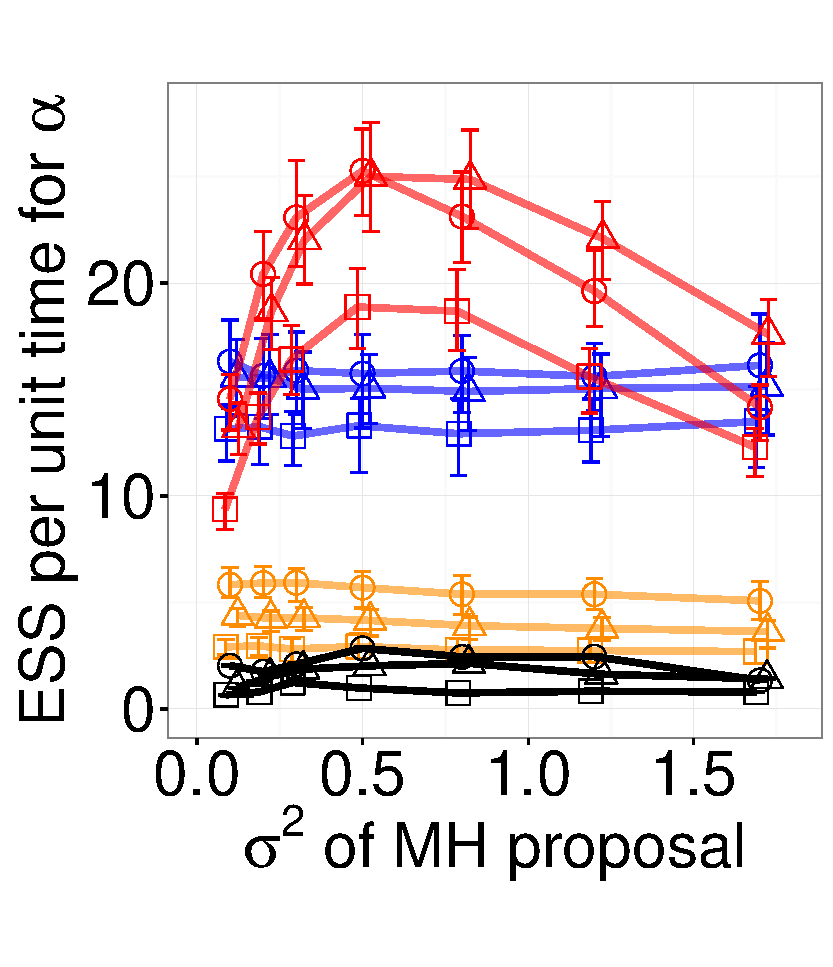
\includegraphics [width=0.90\textwidth, angle=0]{figs/exp_3_alpha.pdf}
      \end{minipage}
  \begin{minipage}[hp]{0.45\linewidth}
  \centering
    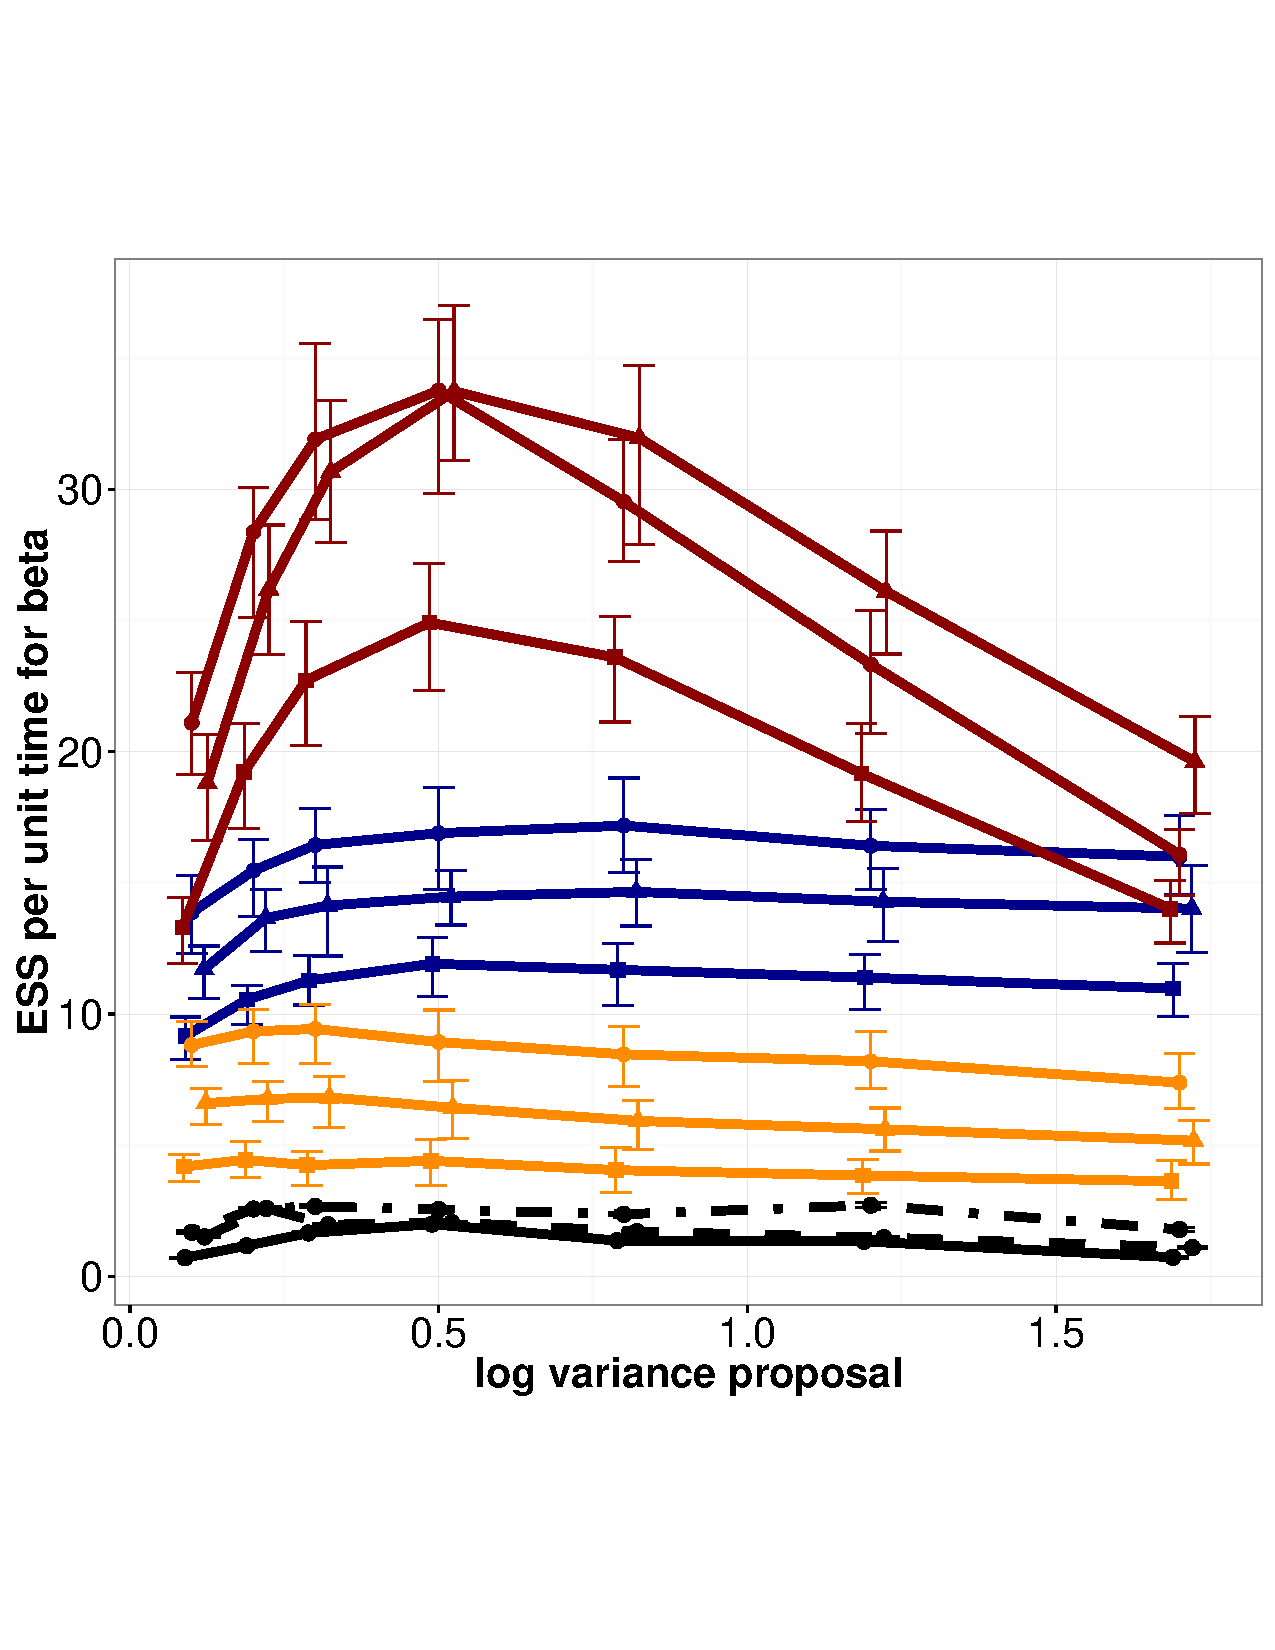
\includegraphics [width=0.90\textwidth, angle=0]{figs/exp_3_beta.pdf}
    \vspace{-0 in}
  \end{minipage}
    \caption{ESS/sec for exp model (dim 3). The left is for $\alpha$, and the right is for $\beta$.}
     \label{fig:ESS_EXP_D3}
  \end{figure}
  In Figure~\ref{fig:ESS_EXP_D3}, Figure~\ref{fig:ESS_EXP_D5}, Figure~\ref{fig:ESS_EXP_D10} we plot the ESS per unit time for the parameters $\alpha$ (left) and $\beta$ (right) as we change the variance of the
  proposal kernel per run, for different methods and different scaling parameters k($k = 1.5, 2, 3$) and different dimensions($p = 3, 5, 10$), where   $k = 1.5$,  $\Omega(\theta, \theta^*) = k \max(\max A(\theta), \max A(\theta^*))$. For particle MCMC, The number of particles can be $5, 10 , 20$. Blue lines are for Gibbs sampler. Red lines are for improved MH. Orange lines are for naive MH. Black lines are for particle MCMC. Lines with dots correspond to $k = 1.5$. Lines with triangle correspond to $k = 2$. Lines with squares correspond to $k = 3$.  The black dot dash lines correspond to $N  = 5$. The dash black lines correspond to $N  = 10$. The solid black lines correspond to $N  = 20$. $N$ is the number of particles. For $k=$ $2$ or $3$, $\Omega(\theta, \theta^*) = \frac{k}{2} (\max A(\theta) + \max A(\theta^*))$. We see that the improved MH algorithm is more efficient i	n these cases with respect to the overall ESS per unit time. We also see that increase the scaling parameter will decrease the efficiency of the improved MH algorithm respect to overall ESS per unit time, when $k > 2$. If we set $\Omega = 1.5 \max(\Omega_{old}, \Omega_{new})$, the performance of the improved MH will not be as good as the case we set $\Omega = 2(\Omega_{old} + \Omega_{new})$ when the proposal log variance is large.\\

In Figure~\ref{fig:HMC_DIM_3}, we plot the ESS per unit time as we change the number of leapfrog jumps in Hamiltonian MCMC for dimension $3$. We consider three different step size for leapfrog step($s = 0.02, 0.05, 0.1$). We 
use the same data for our previous experiment for the case when dimension $3$. We set the $m_1 = m_2 = 1.0$. Because using FFBS to explore the gradient needs a lot of computation, it does not work so well.\\

Figure~\ref{fig:Transition_exp} shows the initial burn-in of our improved MH sampler with this setting for different initializations. The vertical axis shows the number of state transitions in the MJP trajectory of each iteration. This quantity quickly reaches its equilibrium value within a few iterations.\\


In Figure~\ref{fig:TSS}, we plot the ESS per unit time as observation interval and the number of observations both increase when the dimension is $3$ and the scaling parameter k is $2$.We generate different observations on different time intervals. Our observation process was a Gaussian distribution with mean equal to the current state and variance equal to $1$. There are $\cT - 1$ observations uniformly observed between the time interval $(0, \cT)$. $\cT$ can be $10, 20, 50, 100$. We compare the performances of Gibbs sampler and MH sampler with different proposal log variance. Variance can be $0.5, 0.6, 0.7$. The blue line correspond to $0.5$ log variance. The red line correspond to $0.6$ log variance. The orange line correspond to $0.7$ log variance.The black line correspond to Gibbs samper. Gibbs sampler decreases faster than Metropolis Hasting Method, due to the doubling of MJP paths and the parameters. \\

In Figure~\ref{fig:TSS_fix}, we plot ESS per unit time as observation interval increases. We generate different observations on different time intervals. Our observation process was a Gaussian distribution with mean equal to the current state and variance equal to $1$. There are $19$ observations uniformly observed between the time interval $(0, \cT)$. $\cT$ can be $10, 20, 50, 100$. The dimension is $3$ and the scaling parameter $k$ is $2$. We compare the performances of Gibbs sampler and MH sampler with different proposal log variance. Variance can be $0.5, 0.6, 0.7$. The blue line correspond to $0.5$ log variance. The red line correspond to $0.6$ log variance. The orange line correspond to $0.7$ log variance.The black line correspond to Gibbs samper.  Variance can be $0.5, 0.6, 0.7$. Gibbs sampler decreases faster than Metropolis Hasting Method, due to the doubling of MJP paths and the parameters. In addition Gibbs sampler decreases even more faster than previous case when the number of observations is not fixed. \\




Figure~\ref{fig:acc_exp} plots ESS plots the overall  acceptance rate against the log variance of the proposal kernel per run for dimension $3$. 

  \begin{figure}%[b]
  \centering
  \begin{minipage}[!hp]{0.45\linewidth}
  \centering
    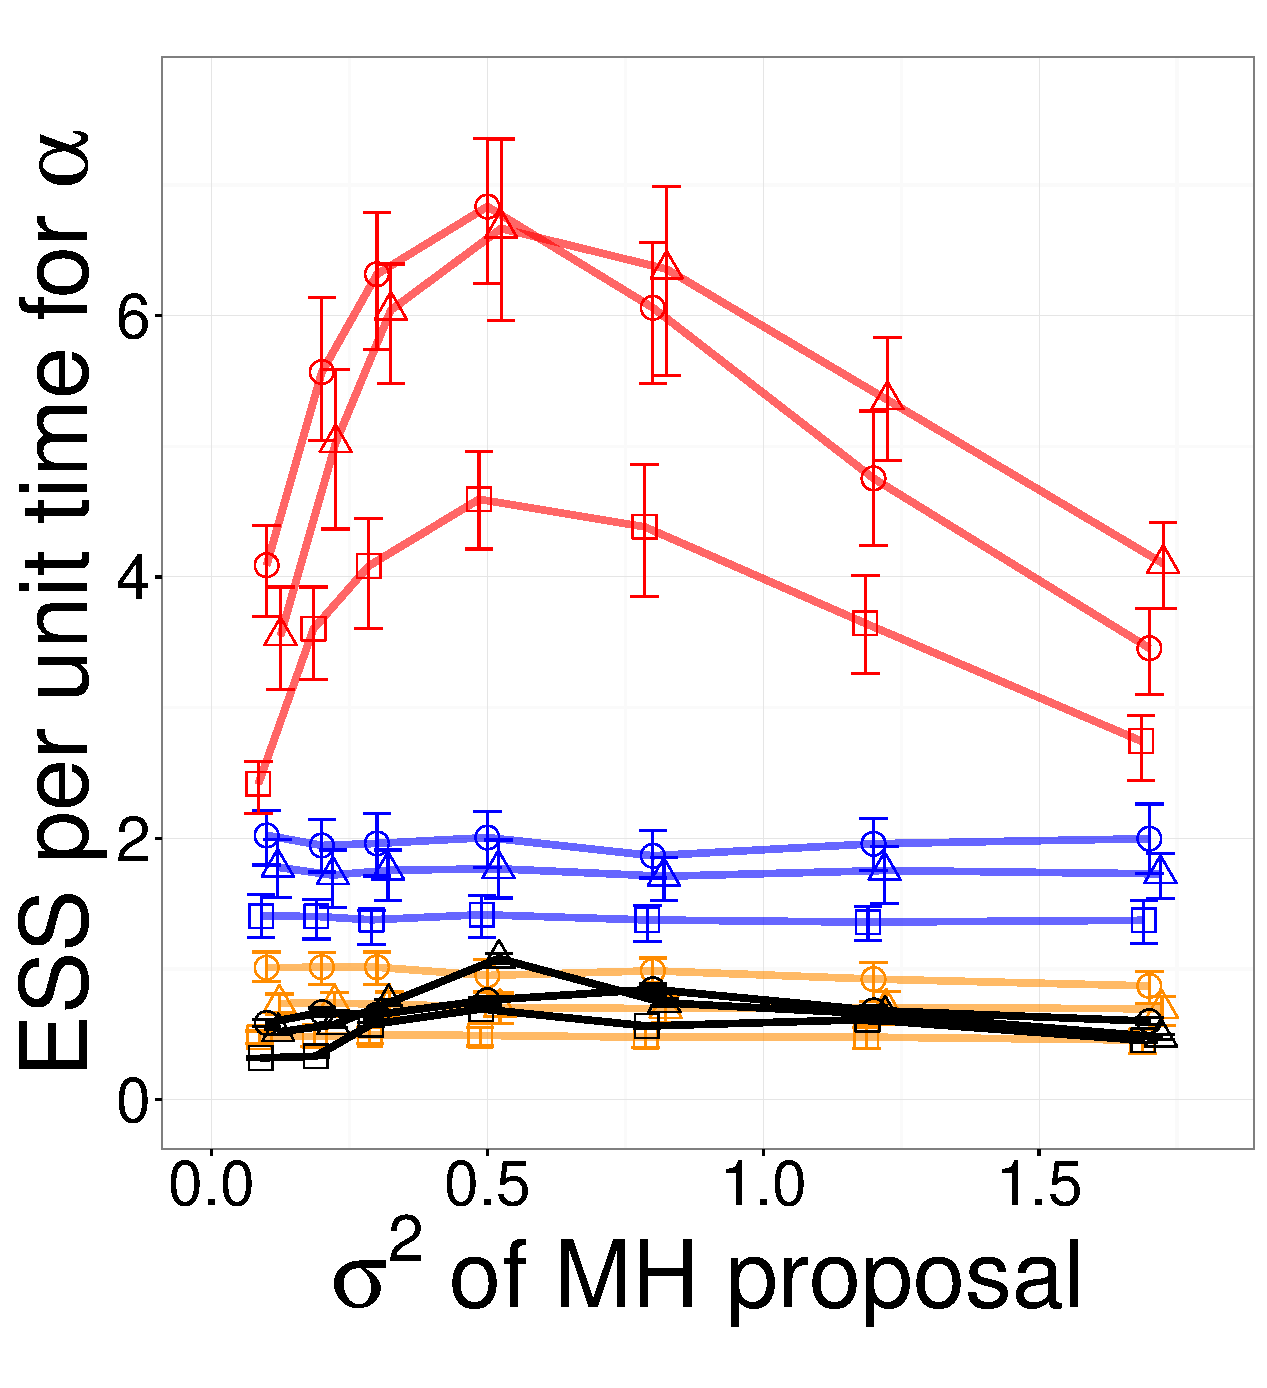
\includegraphics [width=0.90\textwidth, angle=0]{figs/exp_5_alpha.pdf}
      \end{minipage}
  \begin{minipage}[hp]{0.45\linewidth}
  \centering
    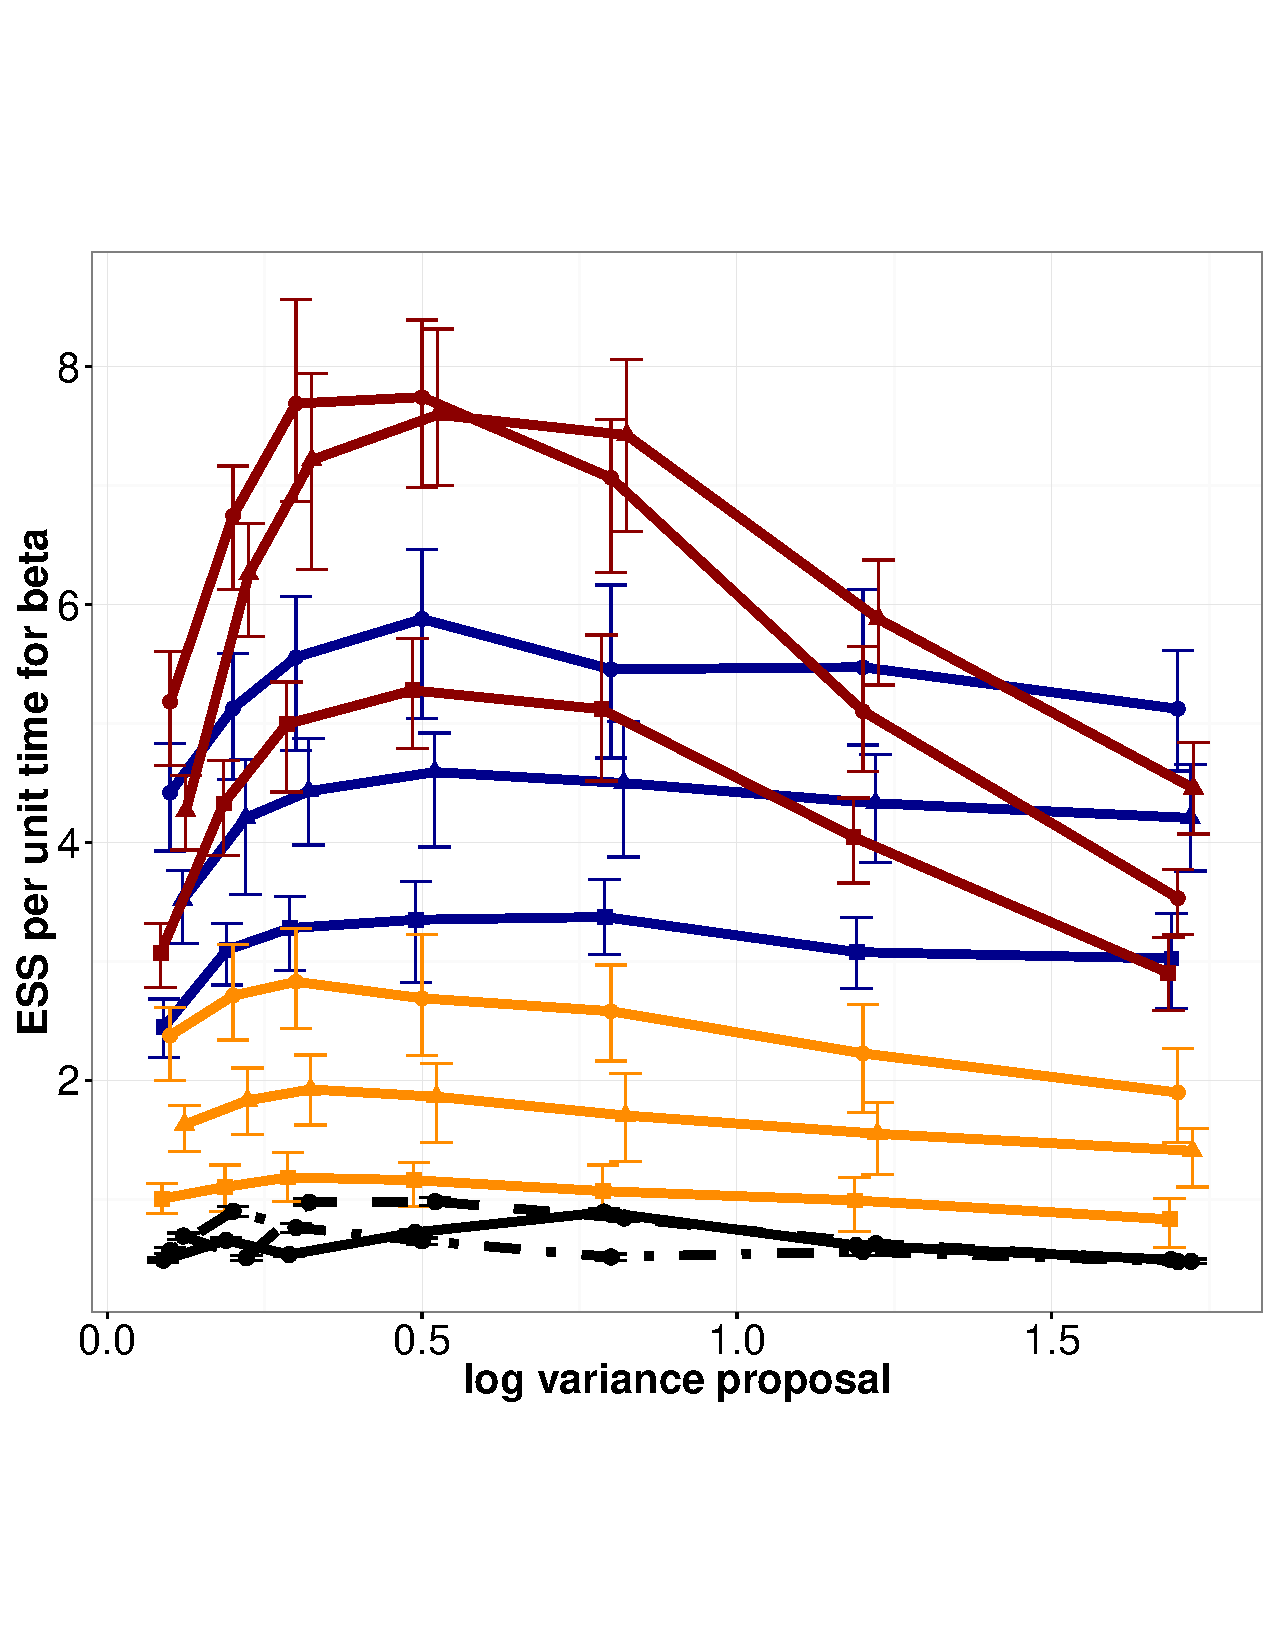
\includegraphics [width=0.90\textwidth, angle=0]{figs/exp_5_beta.pdf}
    \vspace{-0 in}
  \end{minipage}
    \caption{ESS/sec for exp model (dim 5). The left is for $\alpha$, and the right is for $\beta$.}
     \label{fig:ESS_EXP_D5}
  \end{figure}

  \begin{figure}%[b]
  \centering
  \begin{minipage}[!hp]{0.45\linewidth}
  \centering
    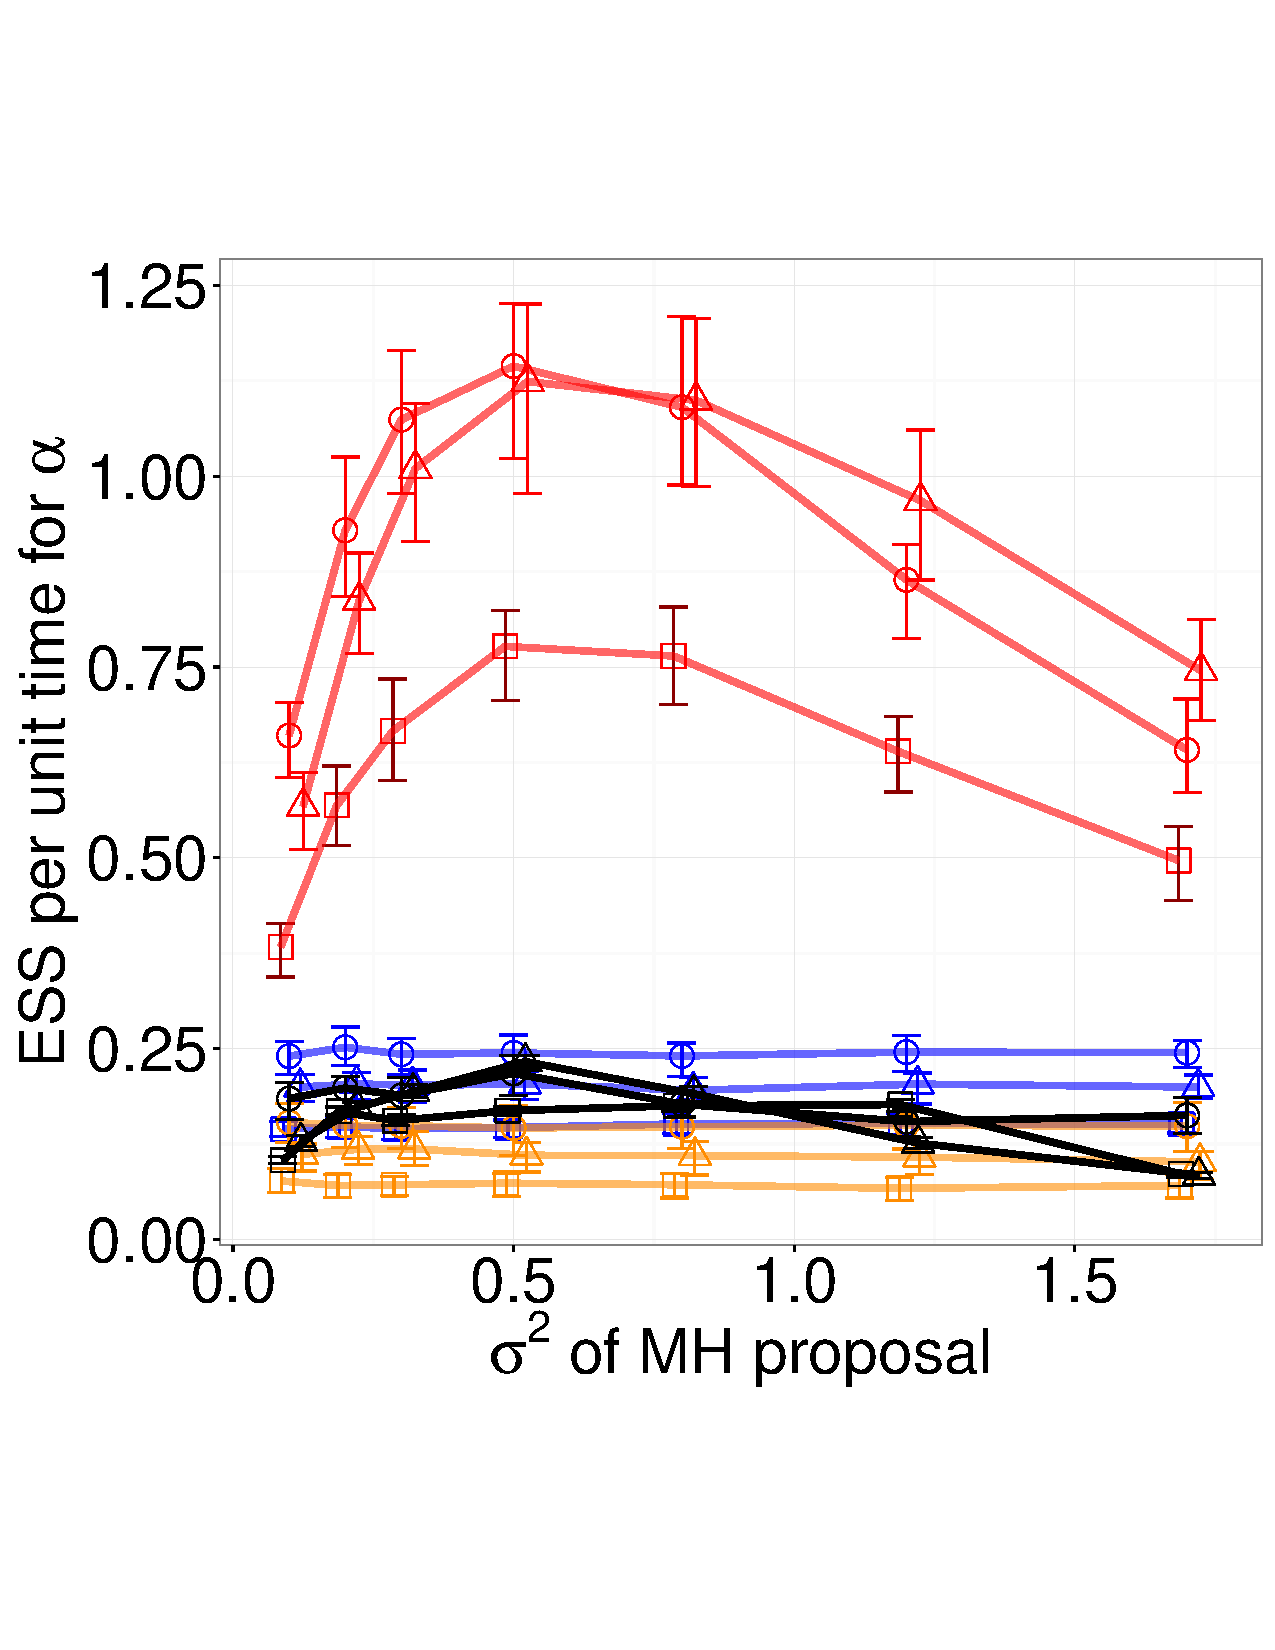
\includegraphics [width=0.90\textwidth, angle=0]{figs/exp_10_alpha.pdf}
      \end{minipage}
  \begin{minipage}[hp]{0.45\linewidth}
  \centering
    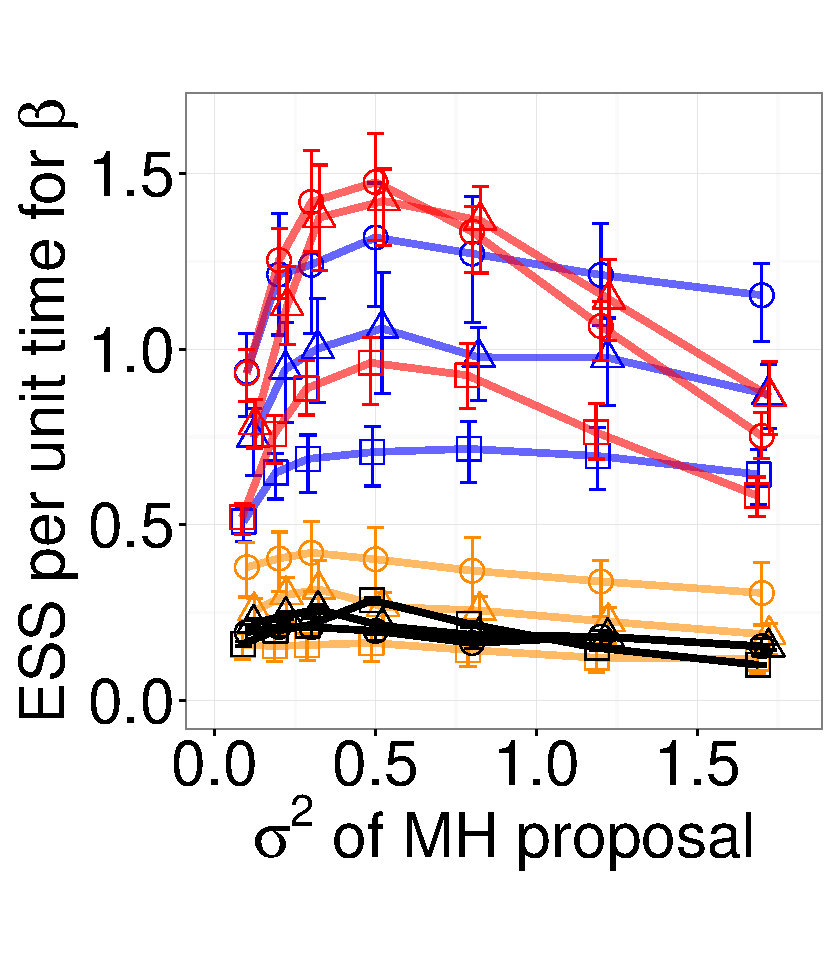
\includegraphics [width=0.90\textwidth, angle=0]{figs/exp_10_beta.pdf}
    \vspace{-0 in}
  \end{minipage}
    \caption{ESS/sec for exp model (dim 10). The left is for $\alpha$, and the right is for $\beta$.}
     \label{fig:ESS_EXP_D10}
  \end{figure}
  
    \begin{figure}%[b]
  \centering
  \begin{minipage}[hp]{0.45\linewidth}
  \centering
    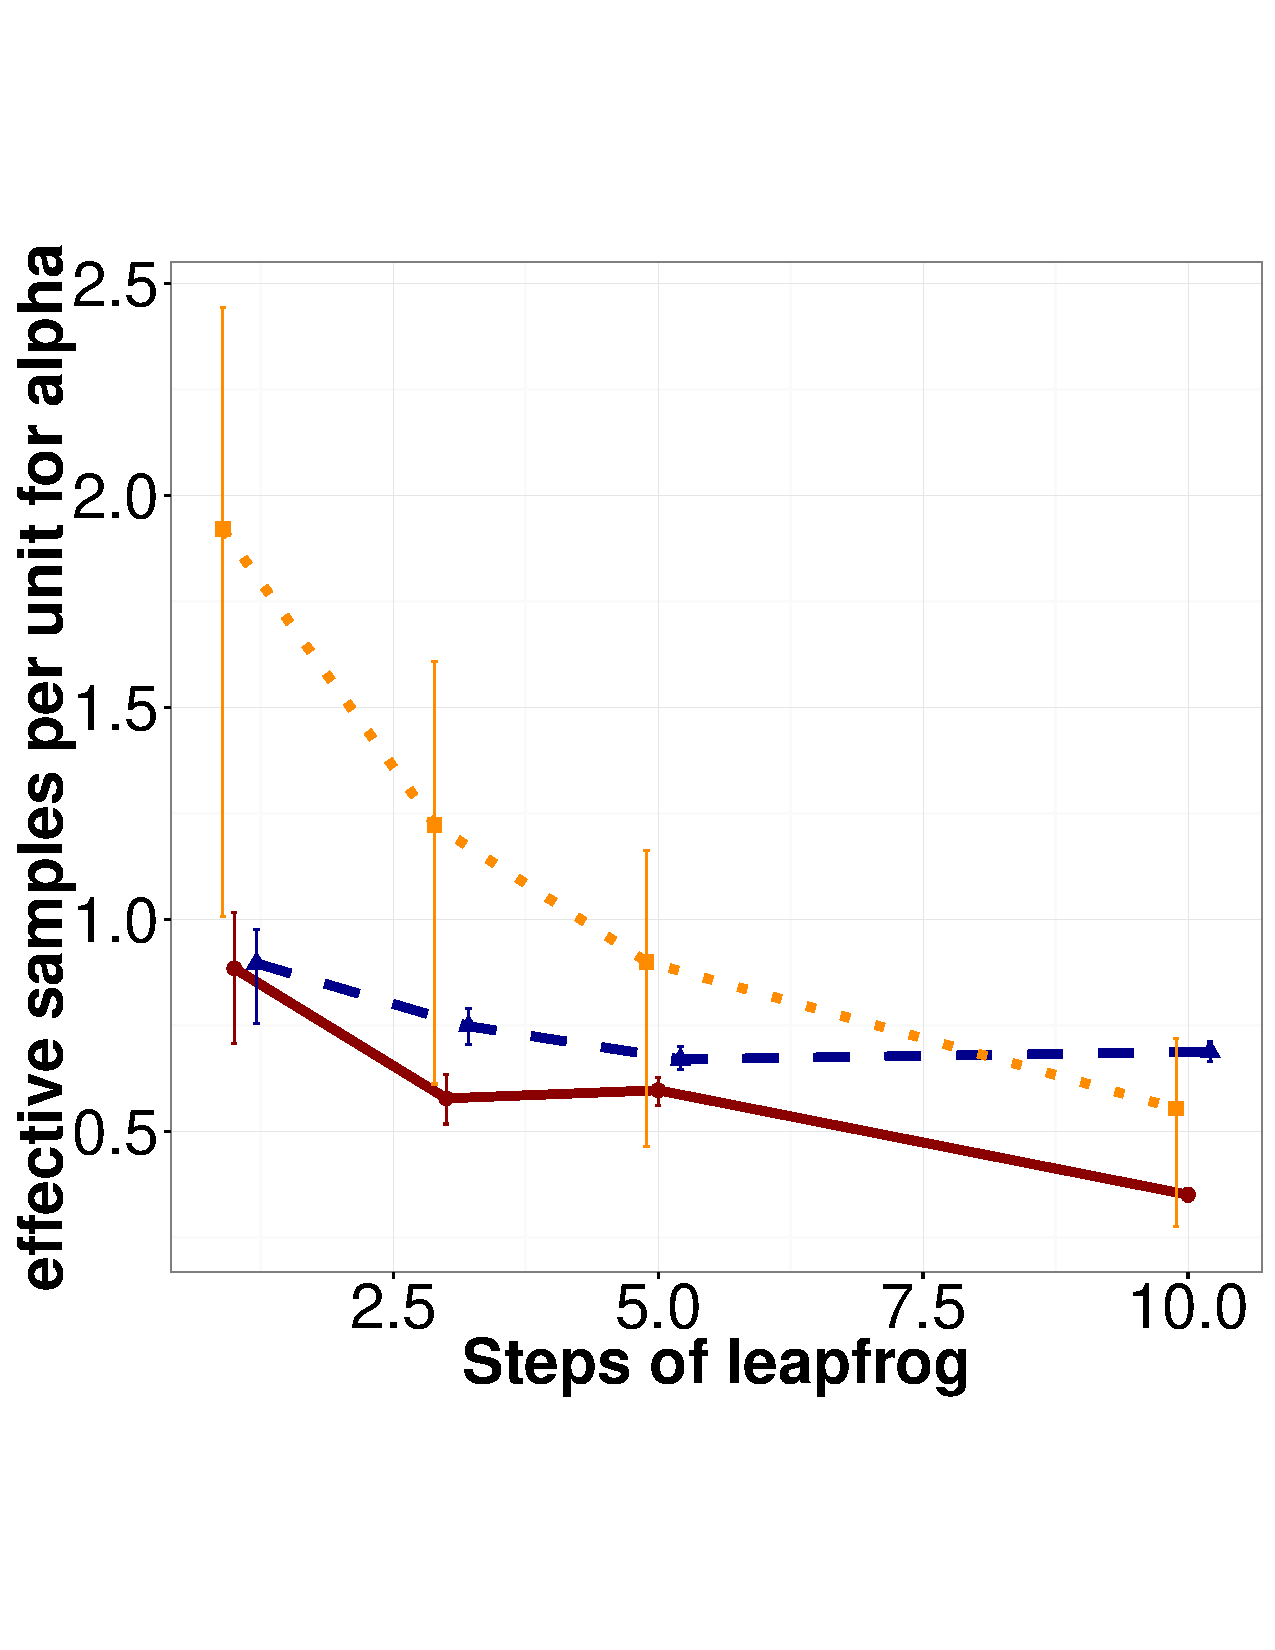
\includegraphics [width=0.90\textwidth, angle=0]{figs/h_alpha.pdf}
      \end{minipage}
  \begin{minipage}[hp]{0.45\linewidth}
  \centering
    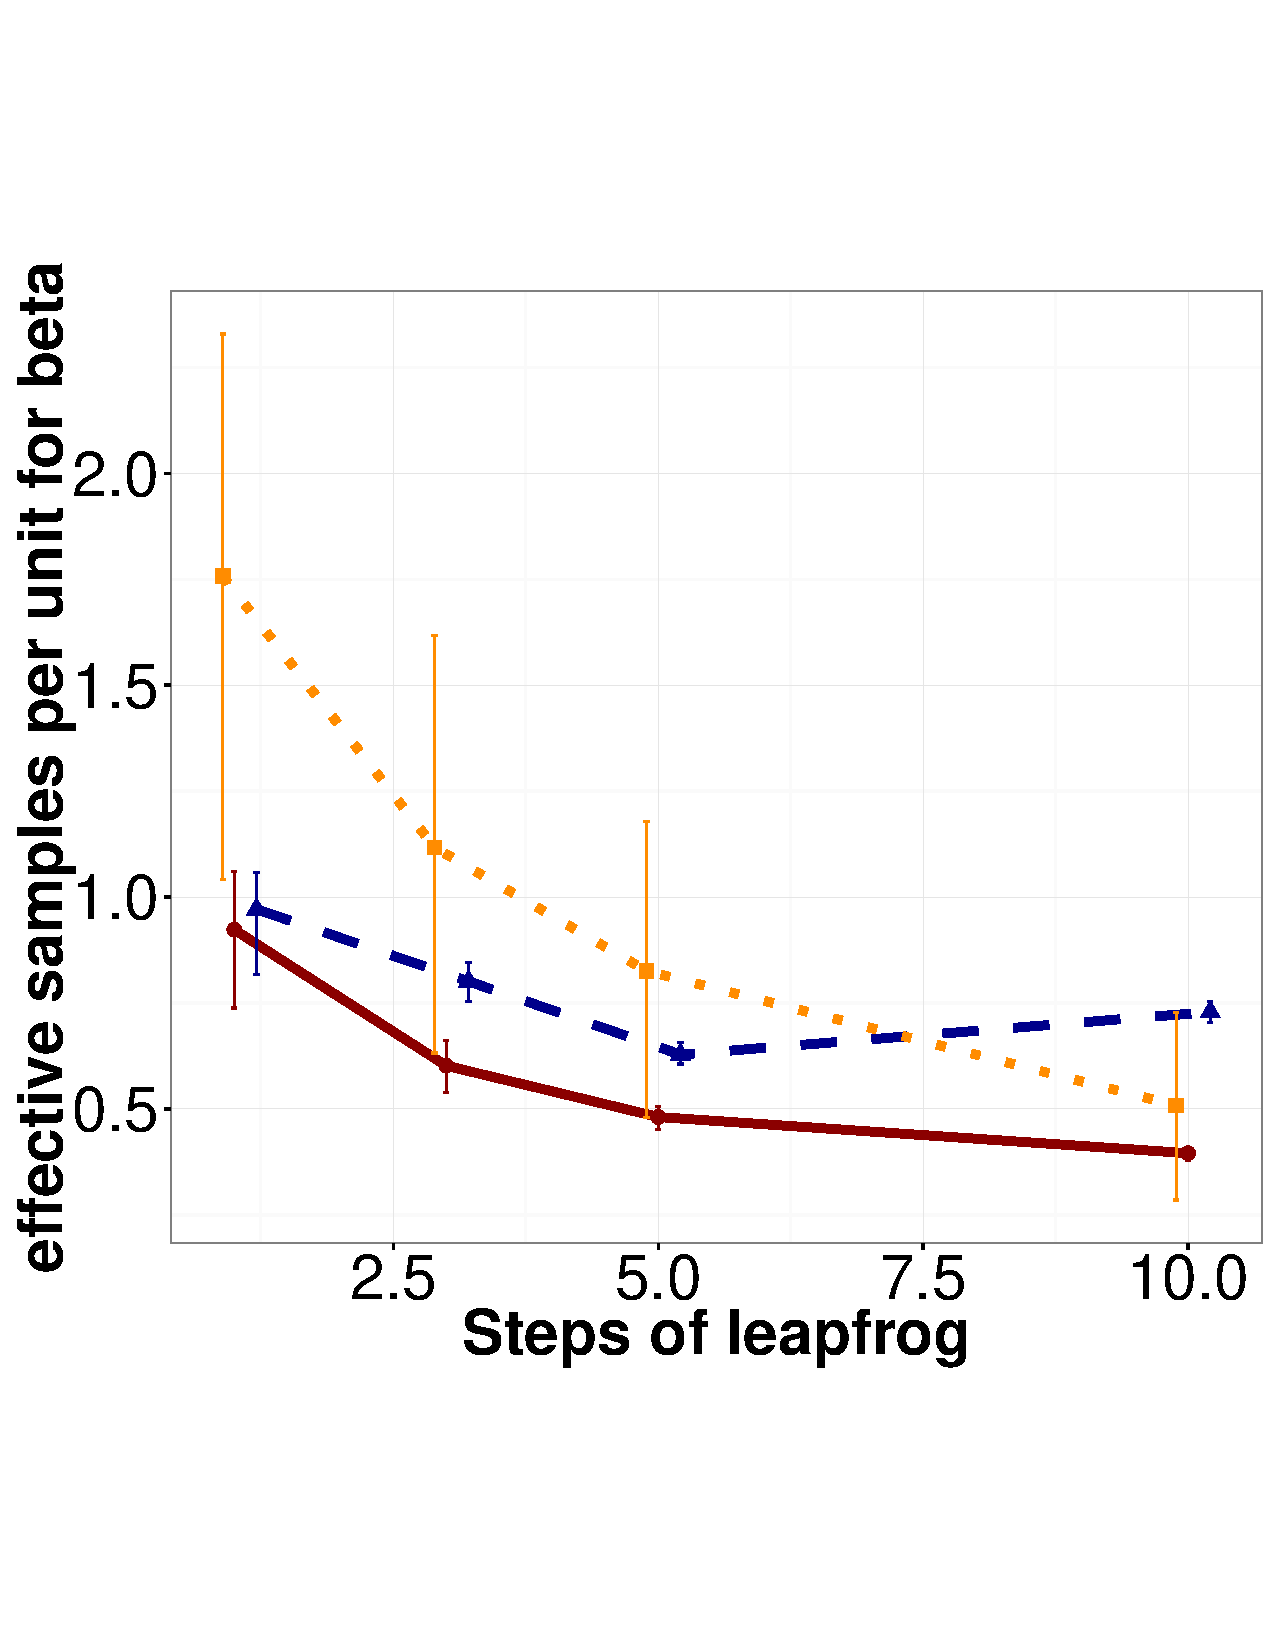
\includegraphics [width=0.90\textwidth, angle=0]{figs/h_beta.pdf}
      \end{minipage}
    \caption{HMC for dim 3}
    \label{fig:HMC_DIM_3}
  \end{figure}
  
  \begin{figure}%[b]
  \centering
  \begin{minipage}[hp]{0.45\linewidth}
  \centering
    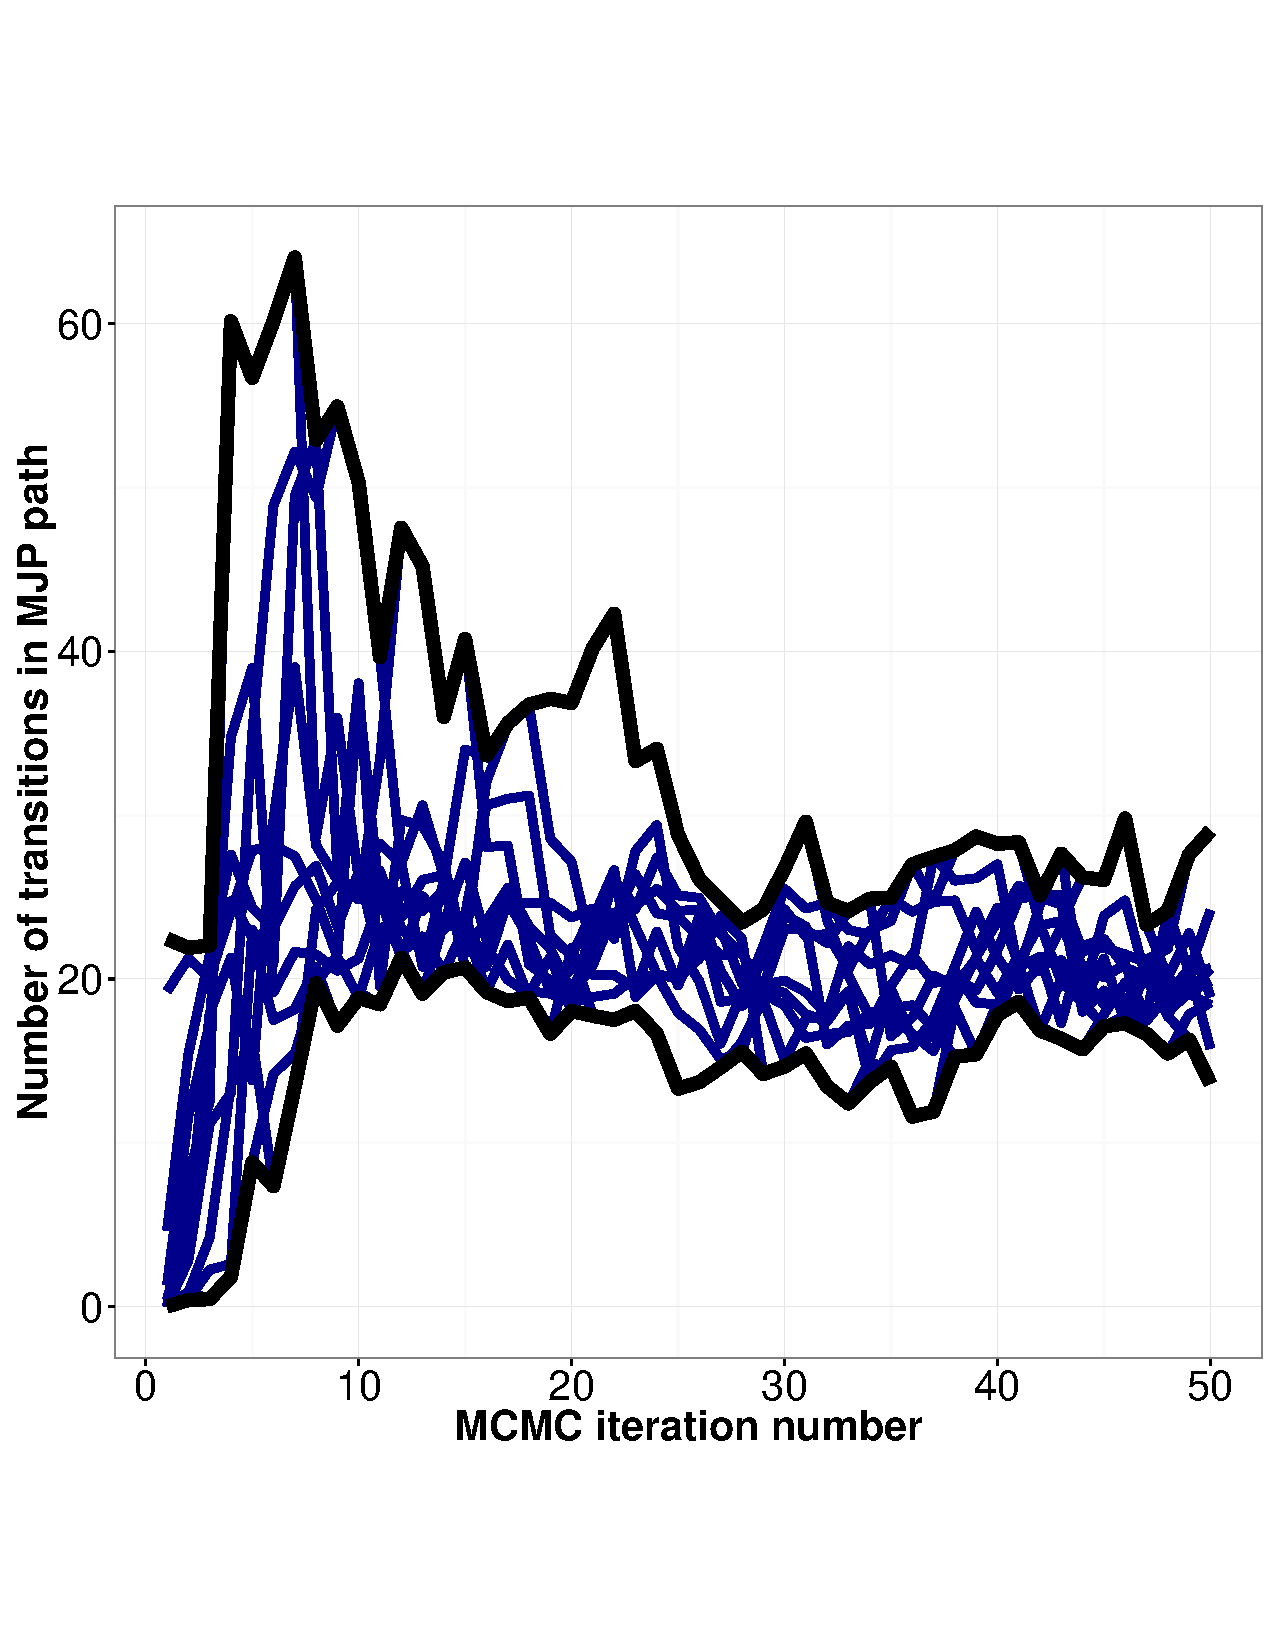
\includegraphics [width=0.90\textwidth, angle=0]{figs/exp3_k2_path_transition.pdf}
      \end{minipage}
    \caption{Trace plot of the number of MJP transitions for different initializatoins.}
	\label{fig:Transition_exp}
  \end{figure}

  \begin{figure}%[b]
  \centering
  \begin{minipage}[hp]{0.45\linewidth}
  \centering
    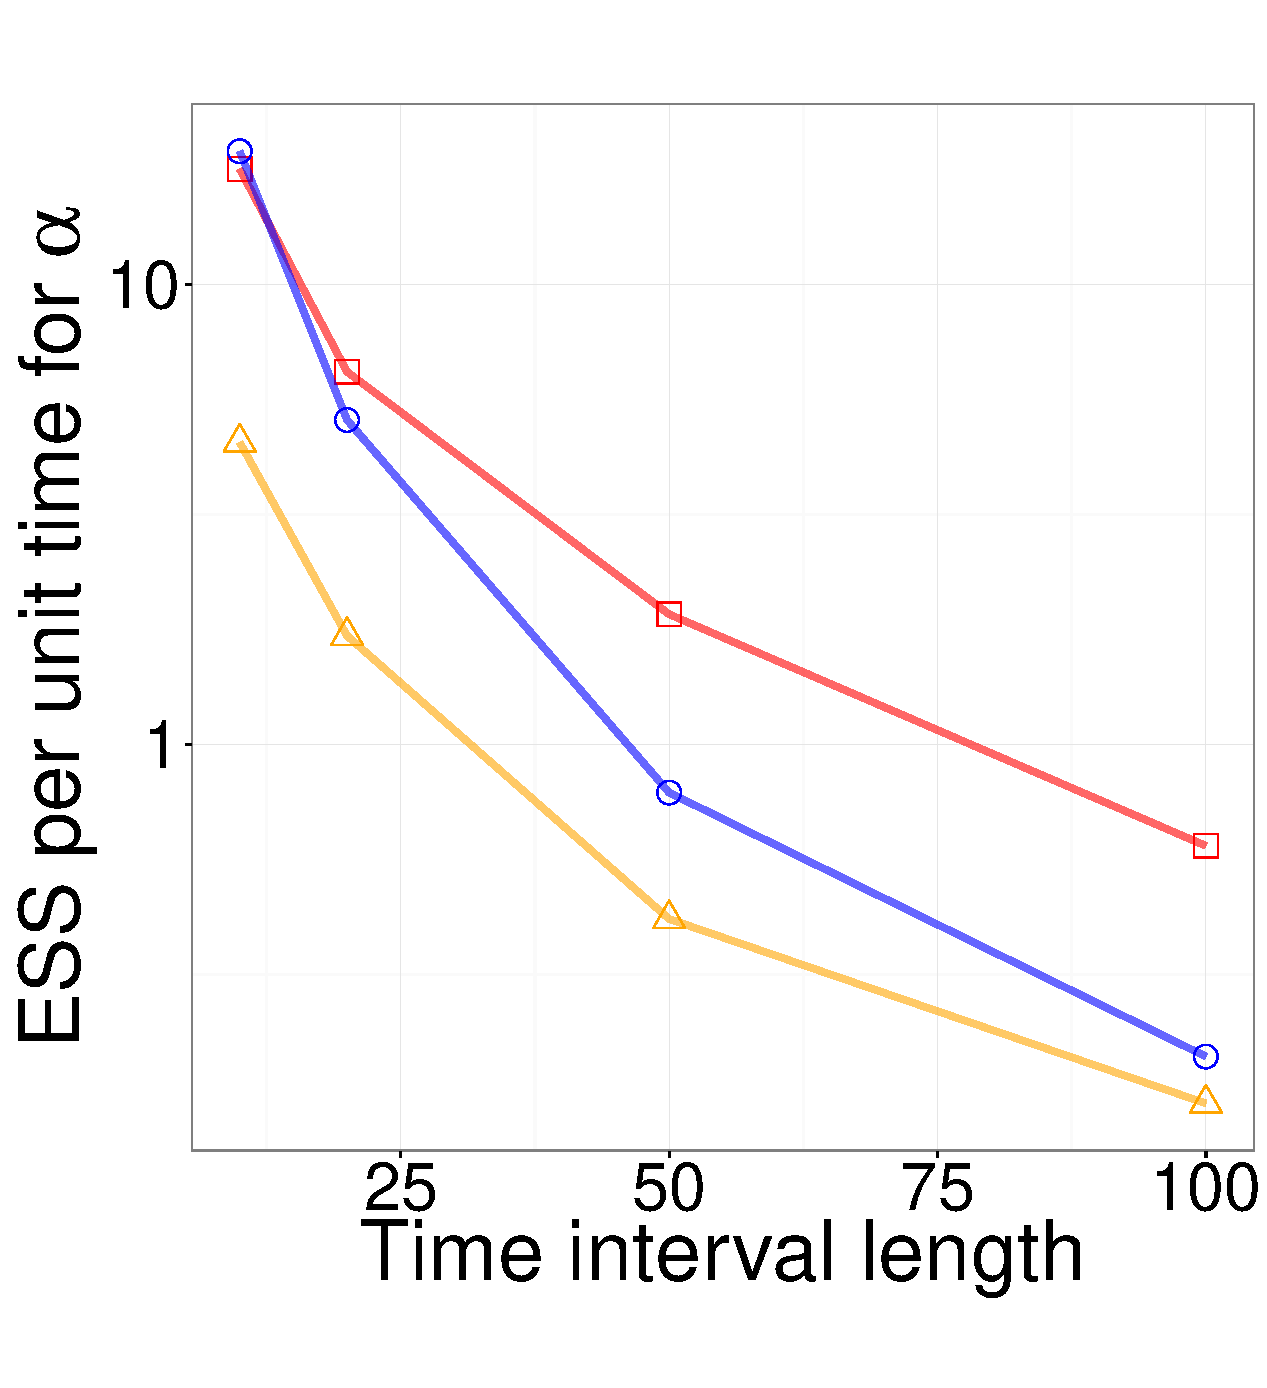
\includegraphics [width=0.90\textwidth, angle=0]{figs/ESS_vs_t_alpha.pdf}
      \end{minipage}
  \begin{minipage}[hp]{0.45\linewidth}
  \centering
    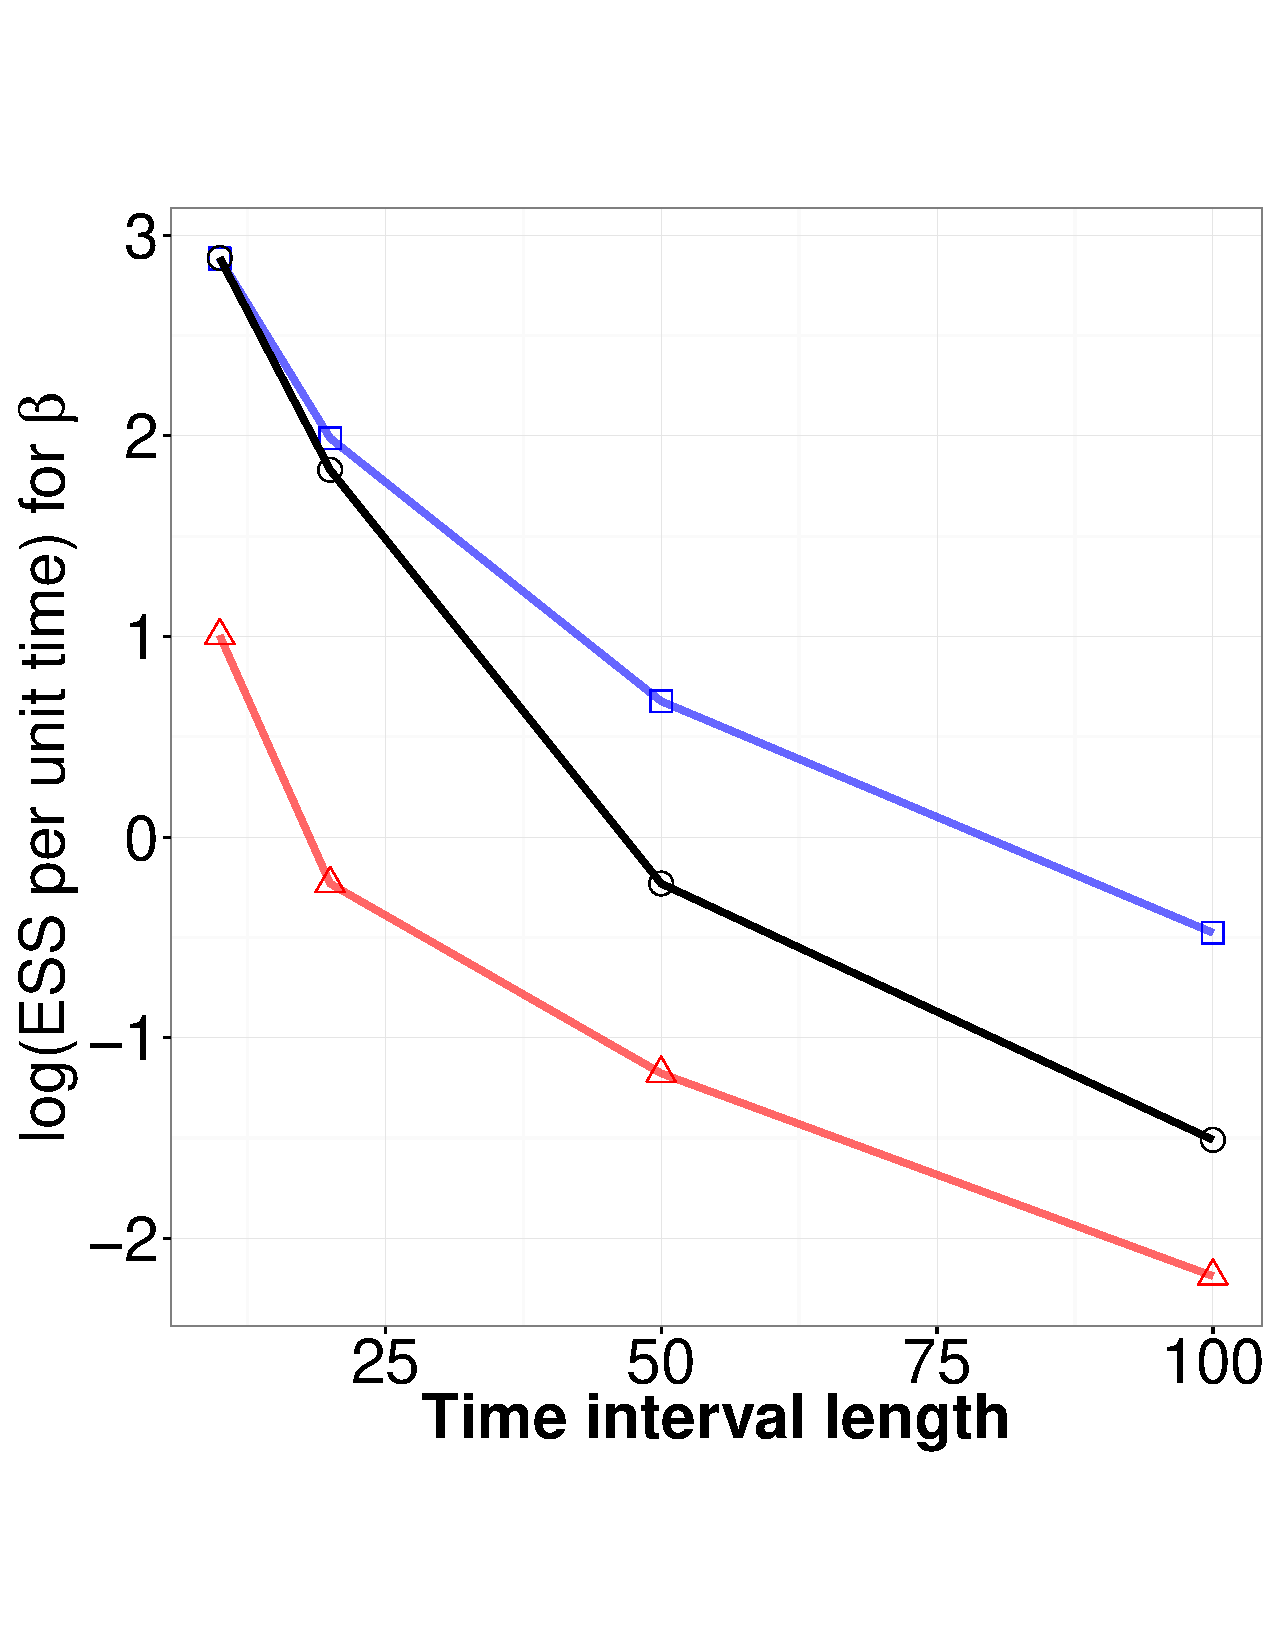
\includegraphics [width=0.90\textwidth, angle=0]{figs/ESS_vs_t_beta.pdf}
    \vspace{-0 in}
  \end{minipage}
    \caption{Time Interval vs. ESS / sec}
     \label{fig:TSS}
  \end{figure}


  \begin{figure}%[b]    
  \centering
  \begin{minipage}[hp]{0.45\linewidth}
  \centering
    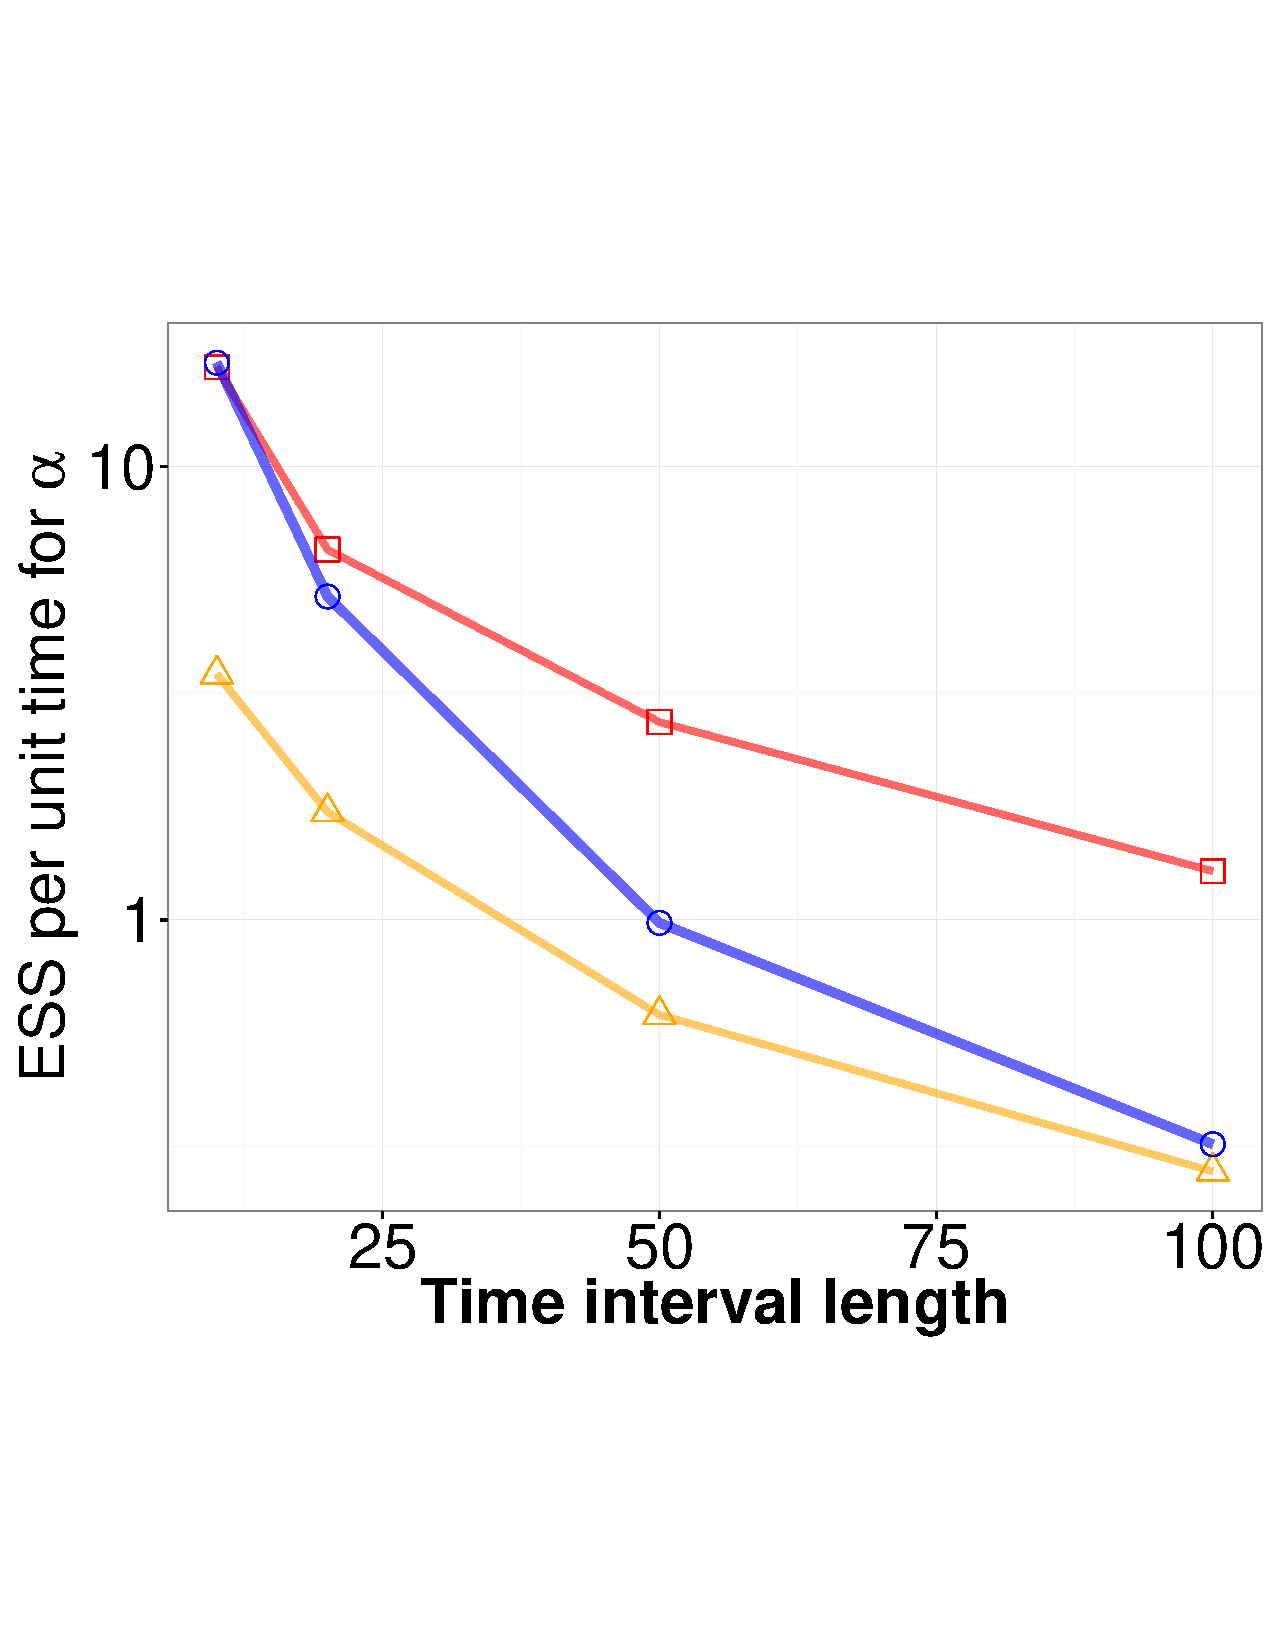
\includegraphics [width=0.90\textwidth, angle=0]{figs/ESS_vs_t_alpha_fixobservation.pdf}
    \end{minipage}
  \begin{minipage}[hp]{0.45\linewidth}
  \centering
    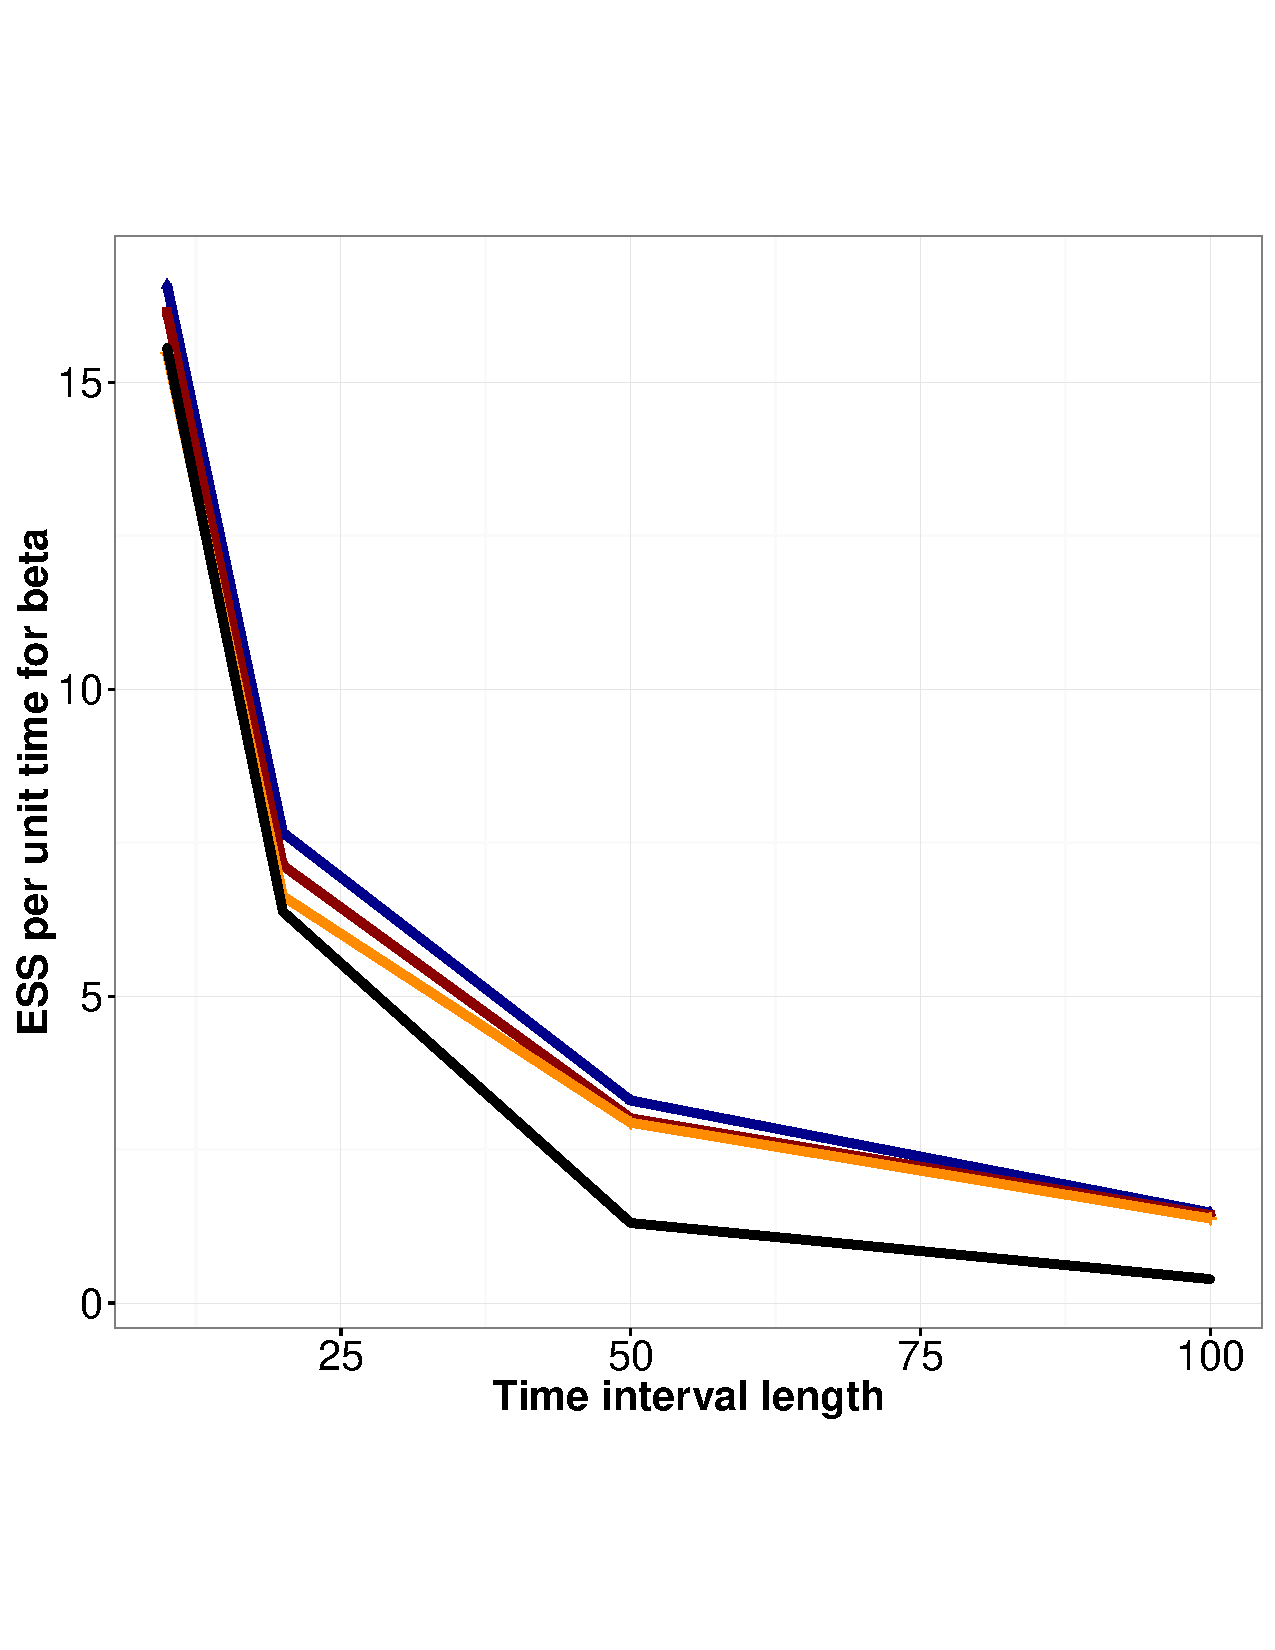
\includegraphics [width=0.90\textwidth, angle=0]{figs/ESS_vs_t_beta_fixobservation.pdf}
    \vspace{-0 in}
  \end{minipage}
    \caption{Time Interval vs. ESS / sec (Number of observations is fixed)}
     \label{fig:TSS_fix}
  \end{figure}




  \begin{figure}%[b]
  \centering
  \begin{minipage}[hp]{0.45\linewidth}
  \centering
    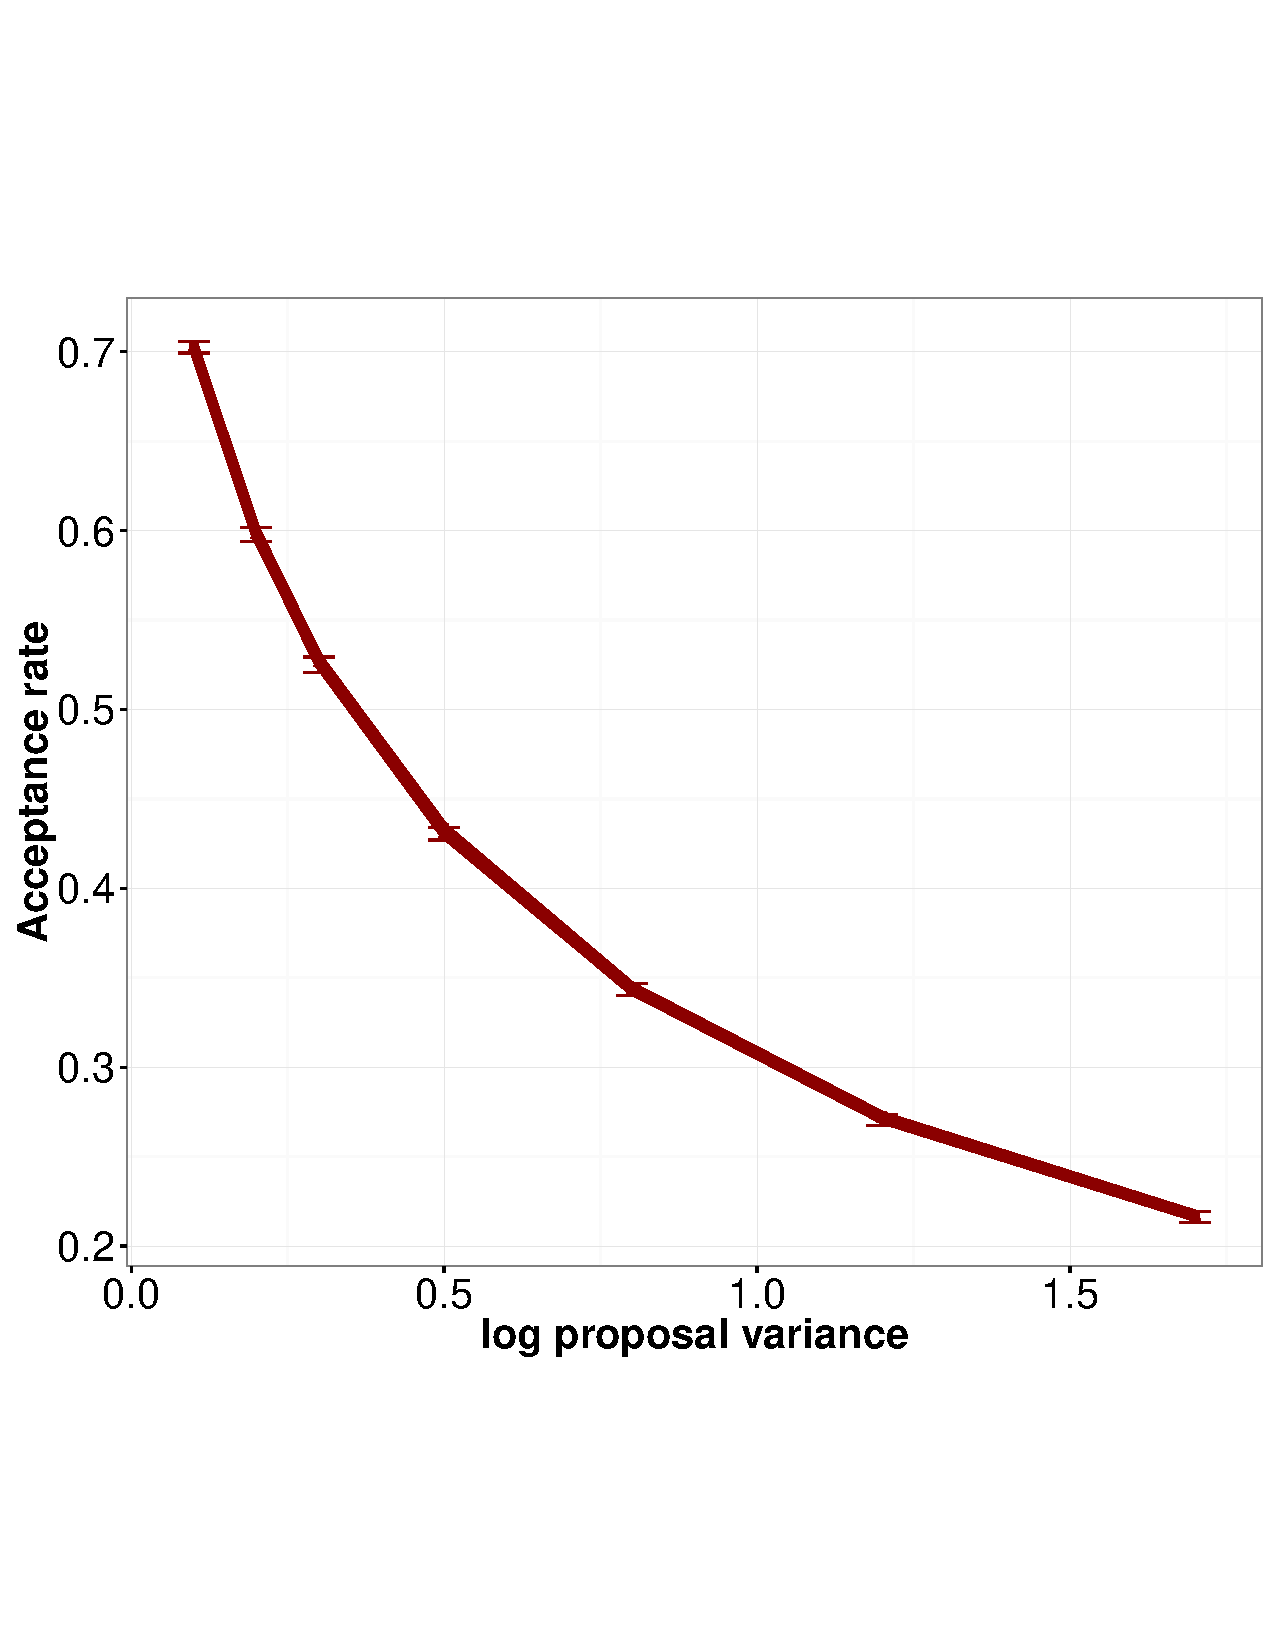
\includegraphics [width=0.90\textwidth, angle=0]{figs/acc_rate_exp_d3.pdf}
      \end{minipage}
    \caption{Acceptance rate for exp model (dim 3)}
	\label{fig:acc_exp}
  \end{figure}


\section{Immigration models with capacity}~

For our next experiment, we consider an $M/M/N/N$ queue. This is a stochastic process whose state space is the set $\{0, 1, 2, 3, ..., N - 1\}$ with elements
corresponds to the number of customers/jobs in the system. Arrivals occur at rate $\alpha$ according to a Poisson process and move the process from state $i$ to $i+1$. 
Service times have an exponential distribution with parameter $i\beta$ in the $M/M/N/N$ queue which move the process from $i$ to $i - 1$. There are $N$ servers, which serve from the front of the queue. 
If there are less than $N$ jobs, some of the servers will be idle. Only $N$ customers can queue at any one time. Any further arrivals to the queue are considered ''lost''. We placed Gamma$(\alpha_0,\alpha_1)$, and Gamma$(\beta_0, \beta_1)$ priors on the parameters $\alpha$, $\beta$, with $(\alpha_0,\alpha_1,\beta_0,\beta_1)$ taking
values $(3,2,5,2)$ respectively. In our experiments, we used random parameters drawn from these prior distributions to construct a transition matrix $A$,
and placing a uniform distribution over states at time $0$, sampled an MJP trajectory.
Our observation process was a Gaussian distribution with mean equal to the current state and variance equal to $1$. There are $19$ observations uniformly observed between the time interval $[0, 20]$.
We consider three settings for number of states, $3, 5$ and $10$. Figure~\ref{q_model} shows the situation with $N$ states.  
  \begin{figure}
  \centering
  \begin{minipage}[hp]{0.6\linewidth}%0.45
  \centering
    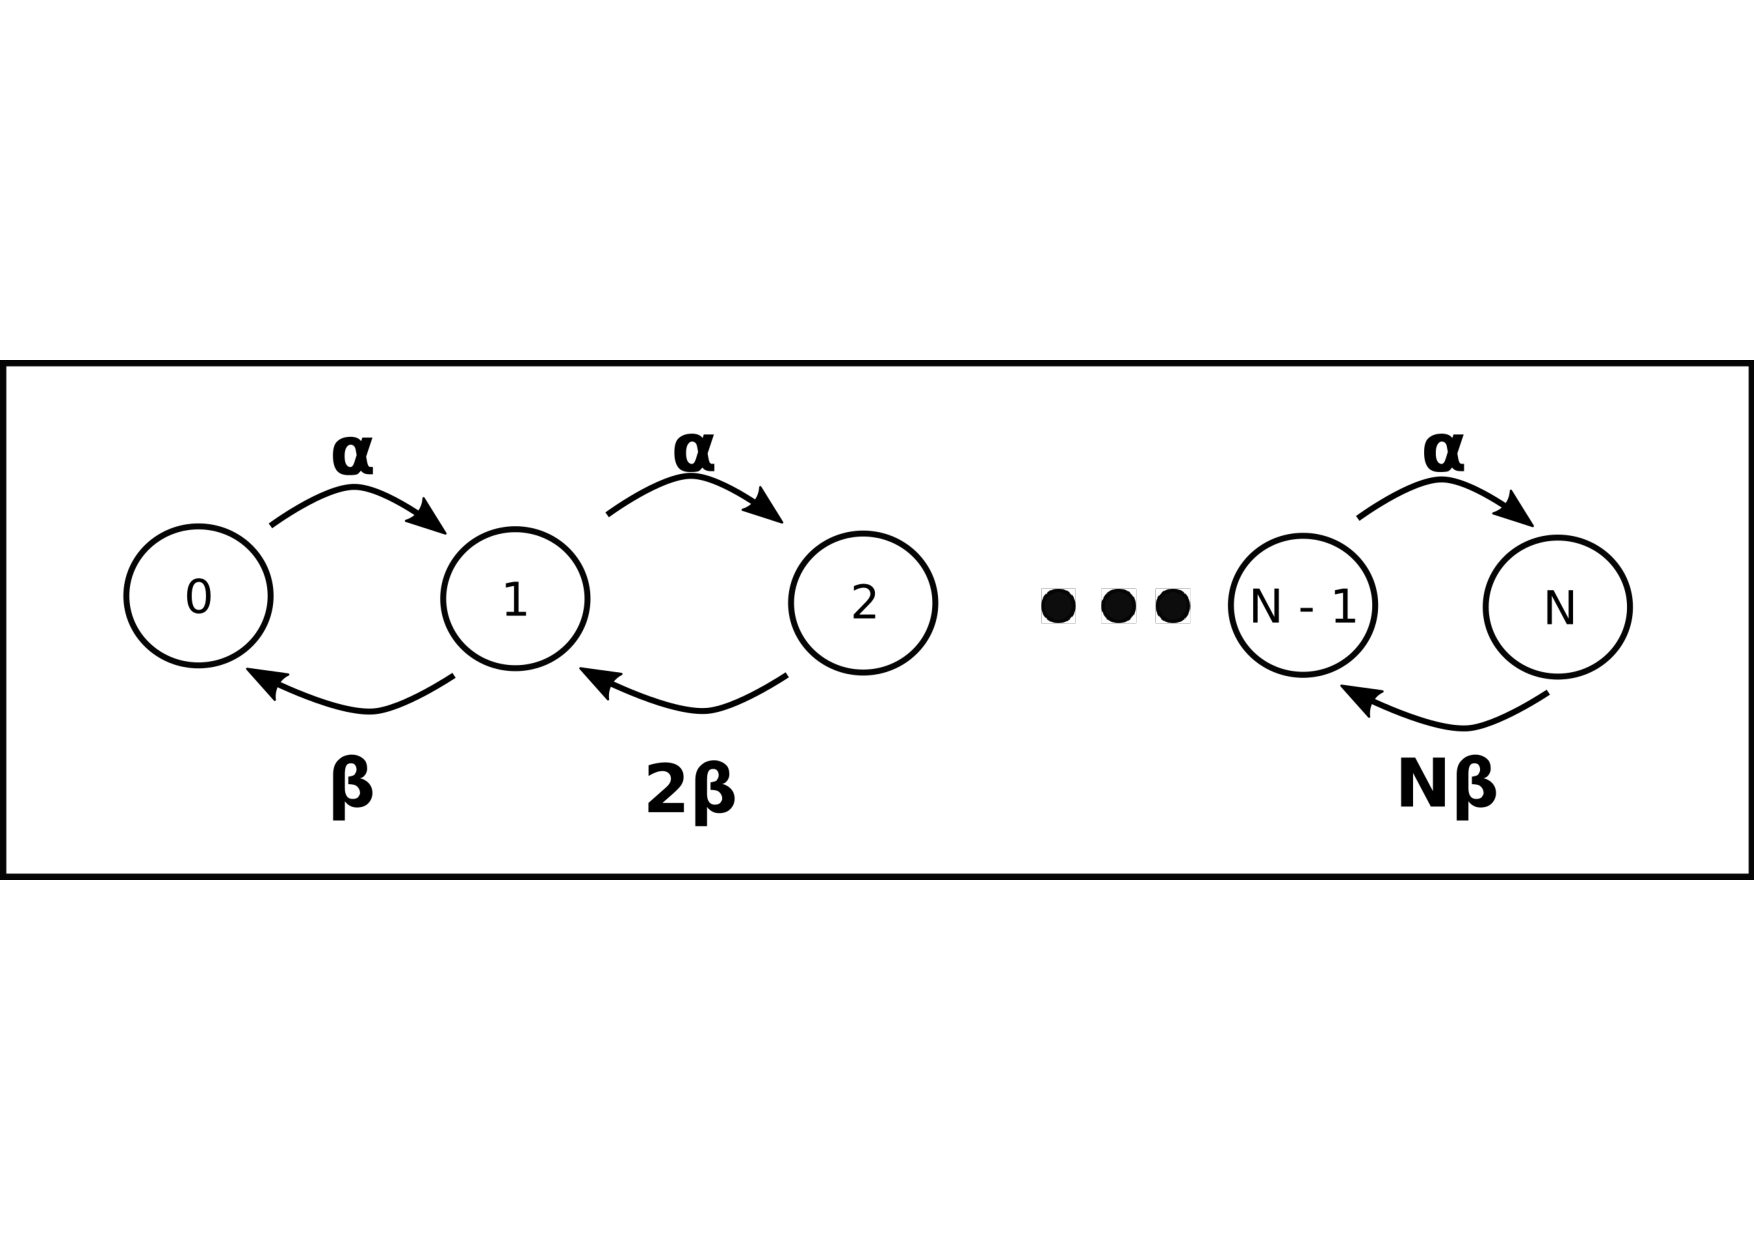
\includegraphics [width=1\textwidth, angle=0]{figs/queue_model.pdf}%0.70
      \end{minipage}
    \caption{queuing model}
	\label{q_model}
  \end{figure}

\noindent Assume: $S = [S_0,S_1, ...,S_N] \;, T = [t_0(t_{start}), t_1,...,t_N, t_{N+1}(t_{end})]$, and y as observations.\\
Now, let's consider a immigration model as follows. State space is $\{0, 1, 2, ..., N - 1\}$, representing the total population. The transition matrix is defined as follows. 
$$A_i =: A_{i,i} = -(\alpha + i\beta), \; \; i =0,1,...,N$$ $$A_{i, i+1} = \alpha, \; \; i =0,1,...,N-1,$$ $$A_{i, i-1}  = \beta, \; \;  i =1,...,N.$$
We already know the conditional density(given $\alpha,\; \beta$) of a MJP trajectory $(s_0, S, T)$ in time interval $[t_{start}, t_{end}]$, with $S=(s_1, s_2,..., s_k)$, $T=(t_1, t_2,..., t_k)$. 
$$f(s_0,S,T| \alpha, \beta) = \prod_{i=0}^{k-1} A_{s_i, s_{i+1}} \exp(\sum_{i=0}^{k} A_{s_i}(t_{i+1} - t_{i})), $$
where $t_0 = t_{start}$, $t_{k+1} = t_{end}.$\\
Let's denote some notations here.\\
$$U(s_0, S, T):= \sum_{i=0}^{k-1} \mathbb{I}_{\{s_{i+1} - s_i = 1\}}.$$
$$D(s_0, S, T):= \sum_{i=0}^{k-1} \mathbb{I}_{\{s_{i+1} - s_i = -1\}}.$$
Call them U and D for short.
Let's denote the total time when the trajectory state stays at state i as $\tau_i$, i.e. $\tau_i = \sum_{j=0}^{k} (t_{j+1} -t_j)\mathbb{I}_{\{s_j = i\}}$, then $\sum_{i=0}^k (t_{i+1} - t_i)s_i = \sum_{i=0}^N \tau_ii.$\\

$$f(s_0,S,T| \alpha, \beta) = \exp(-\alpha(t_{end} - t_{start}- \tau_N) )\alpha^U \cdot  \exp((-(\sum_{i=0}^k (t_{i+1} - t_i)s_i)\beta) \prod_{i=1}^N i^{\sum_{j=0}^{k-1}\mathbb{I}_{s_{j+1} = i -1 \;,  s_j = i} }   \beta^D$$\\
If we assume the prior of $\alpha$, and $\beta$ are $Gamma(\mu,\lambda)$, $Gamma(\omega, \theta)$, which are independent with each other. \\
$$p(\alpha) = \frac{\lambda^\mu}{\Gamma(\mu)}\alpha^{\mu -1}e^{-\lambda \alpha}. $$
$$p(\beta) = \frac{\theta^\omega}{\Gamma(\omega)}\beta^{\omega -1}e^{-\theta \beta}. $$
Then we can get the posterior distribution $$f(\alpha, \beta | s_0,S,T)$$ as follows.
$$ f(\alpha, \beta | s_0,S,T) \propto \exp(-(\lambda + t_{end} - t_{start}- \tau_N)\alpha) \alpha^{\mu + U -1} \cdot \exp(-(\sum_{i=0}^k (t_{i+1} - t_i)s_i + \theta)\beta) \beta^{\omega+ D -1}.$$
It means that the posterior distributions of $\alpha$, $\beta$ are still independent. \\
$\alpha | s_0,S,T$ is following $Gamma(\mu+ U,\lambda + t_{end} - t_{start}- \tau_N)$\\
$\beta | s_0,S,T$ is following $Gamma(\omega+ D,\theta + \sum_{i=0}^k (t_{i+1} - t_i)s_i)$, which is equivalent to $Gamma(\omega+ D,\theta +\sum_{i=0}^N \tau_ii)$\\
Such immigration models have perfectly conjugate posterior distributions when we assign $\gamma$ priors to $\alpha$ and $\beta$. We apply our Metropolis Hasting algorithms on such models to compare the performance with the performance of Gibbs Sampling algorithm.
\subsection{Experiments}

In the following, we evaluate a Python implementation of our algorithms compared to other exact samplers which include Gibbs sampler and Particle MCMC sampler. We consider three different dimensions which are $3$, $5$, and $10$ and three different $k's$ which are $1.5$, $2$, and $3$. We generated random parameters $\alpha$, $\beta$ from prior distributions ($Gamma(3,2), Gamma(5, 2)$), and used this to construct the transition matrix A. Then we generate an MJP trajectory with a uniform initial distribution over states. The state of this MJP trajectory was observed via a Normal distribution with mean equal to the value of state and variance 1, and posterior samples given the observations were produced by a Python implementation of our algorithm. 100 MCMC runs were performed, each run consisting of 10000(Varies among different dimensions) iterations. For each run, the number of transitions as well as the time spent was calculated, and effective sample sizes (ESSs) of these statistics (the number of independent samples with the same `information' as the correlated MCMC samples) were calculated using R-CODA (Plummer et al., 2006). The overall ESS of a run is defined to be the mean ESS across all these ESSs.

  In Figure~\ref{fig:ESS_Q_D3}, Figure~\ref{fig:ESS_Q_D5}, Figure~\ref{fig:ESS_Q_D10} we plot the ESS per unit time for the parameters $\alpha$ (left) and $\beta$ (right) as we change the variance of the
  proposal kernel per run, for different methods and different scaling parameters k($k = 1.5, 2, 3$) and different dimensions($p = 3, 5, 10$), where   $k = 1.5$,  $\Omega(\theta, \theta^*) = k \max(\max A(\theta), \max A(\theta^*))$. Blue lines are for Gibbs sampler. Red lines are for improved MH. Orange lines are for naive MH. Black lines are for particle MCMC. Lines with dots correspond to $k = 1.5$. Lines with triangle correspond to $k = 2$. Lines with squares correspond to $k = 3$. For $k=$ $2$ or $3$, $\Omega(\theta, \theta^*) = \frac{k}{2} (\max A(\theta) + \max A(\theta^*))$. We see that the improved MH algorithm is more efficient i	n these cases with respect to the overall ESS per unit time. We also see that increase the scaling parameter will decrease the efficiency of the improved MH algorithm respect to overall ESS per unit time, when $k > 2$. If we set $\Omega = 1.5 \max(\Omega_{old}, \Omega_{new})$, the performance of the improved MH will not be as good as the case we set $\Omega = 2(\Omega_{old} + \Omega_{new})$ when the proposal log variance is large.\\


Figure~\ref{fig:ESS_Q_TRANSITION} shows the initial burn-in of our improved MH sampler with this setting for different initializations. The vertical axis shows the number of state transitions in the MJP trajectory of each iteration. This quantity quickly reaches its equilibrium value within a few iterations.\\
Figure~\ref{fig:hist} shows posterior distributions for $P(\theta | X)$(red), $P(\theta | S, T, X)$(green), $P(\theta | W, X)$(blue). We run $10000$ iterations. The first $5000$ are treated as burn in period. We fix $V_{5000}, W_{5000}$ and then sample $\theta$ from $P(\theta | V_{5000}, W_{5000}, X)$ and sample $\theta$ from $P(\theta | W_{5000}, X)$. We keep updating $S$ and $T$ for sampling from $P(\theta | X)$. We sample another $5000$ $\theta$s to draw the histograms. We can find that $P(\theta | S, T, X)$ and $P(\theta | W, X)$ are both very concentrated which implies the coupling.
  \begin{figure}%[b]
  \centering
  \begin{minipage}[hp]{0.45\linewidth}
  \centering
    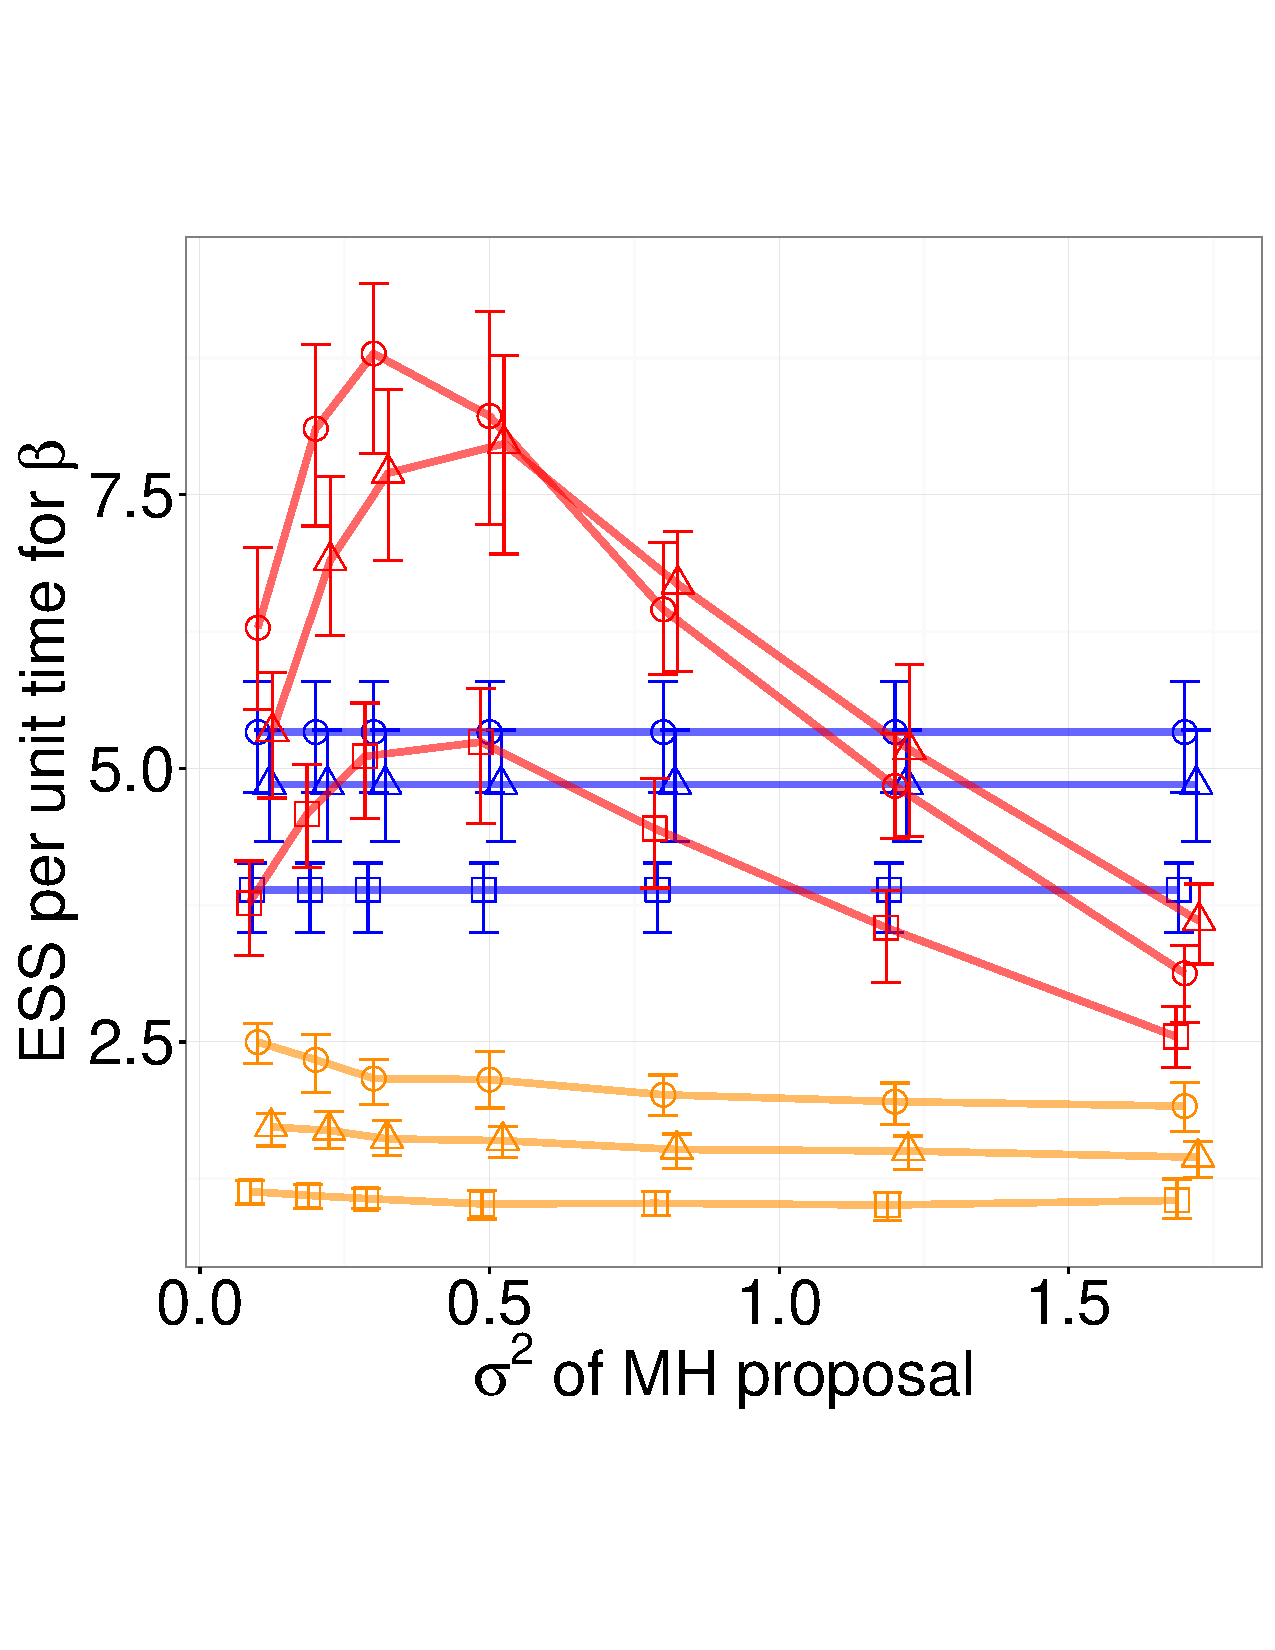
\includegraphics [width=0.90\textwidth, angle=0]{figs/q_3_alpha.pdf}
      \end{minipage}
  \begin{minipage}[hp]{0.45\linewidth}
  \centering
    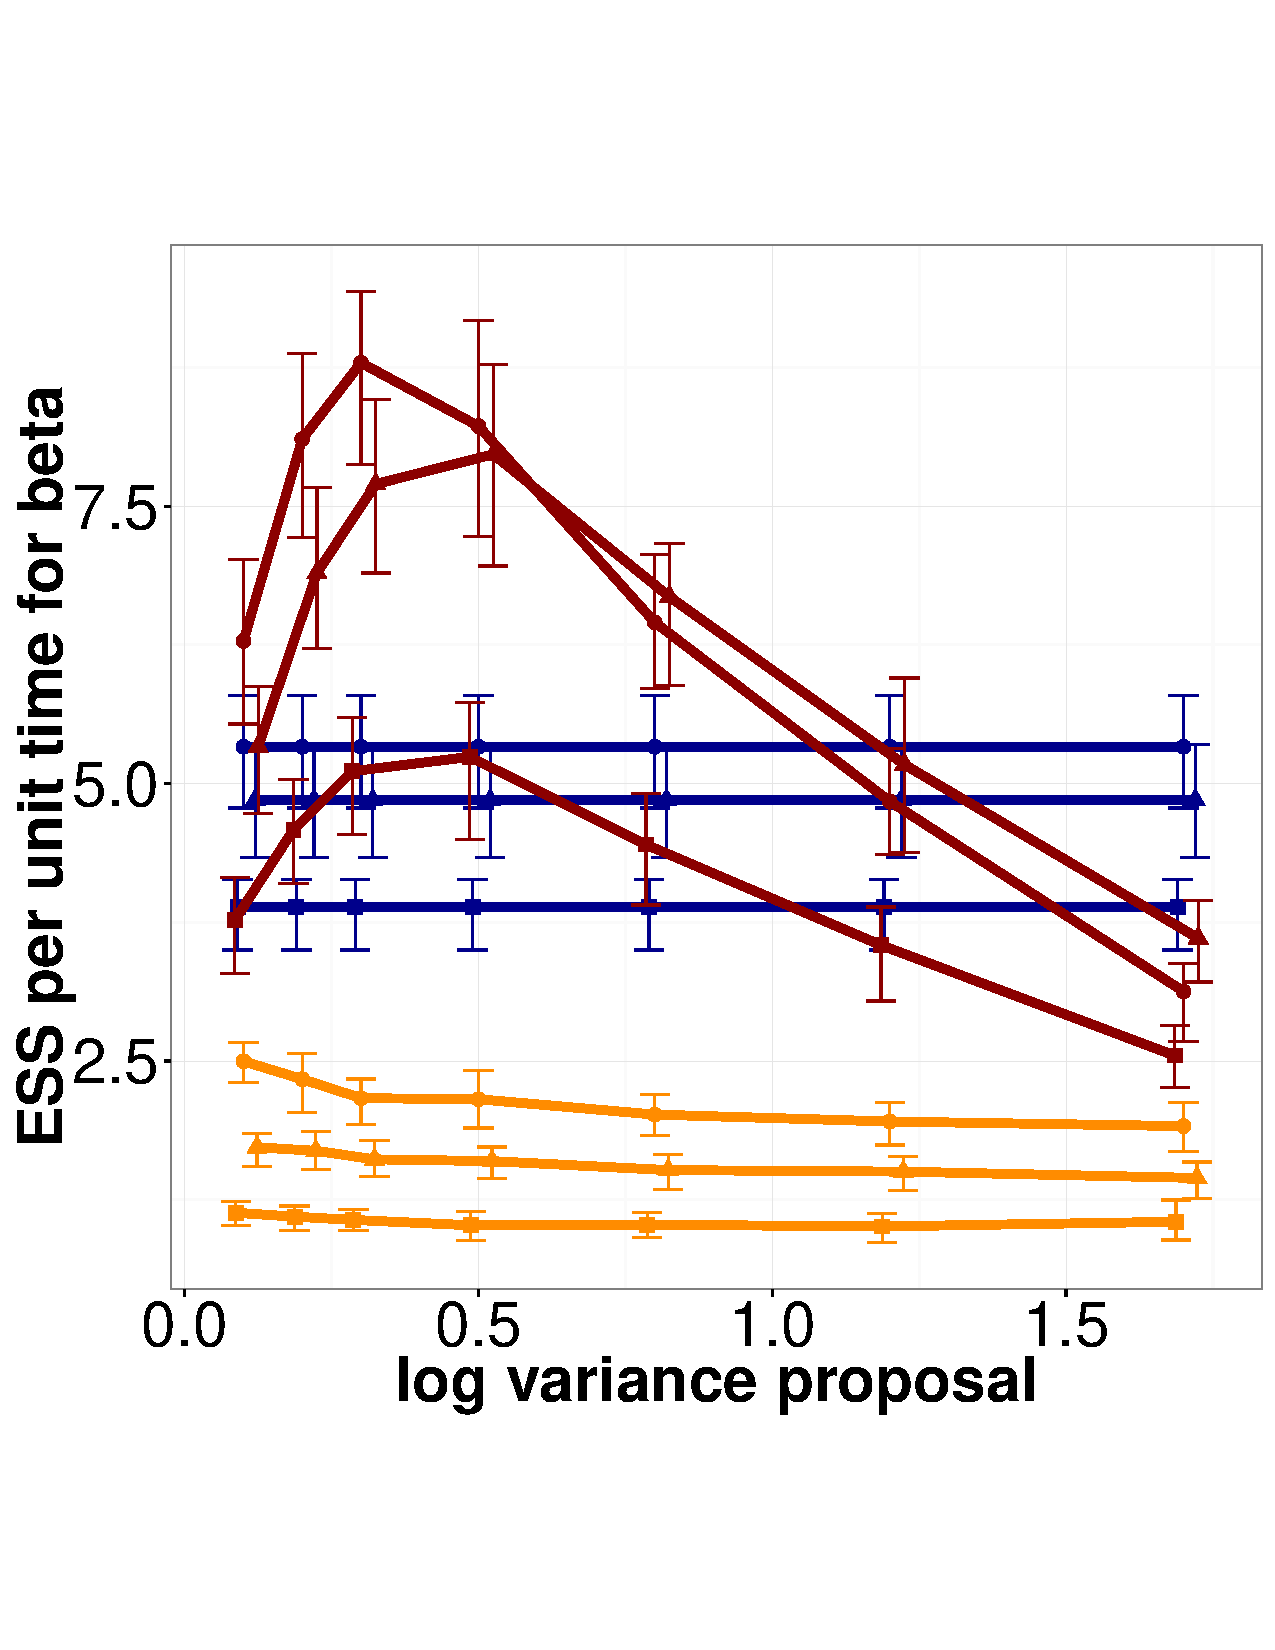
\includegraphics [width=0.90\textwidth, angle=0]{figs/q_3_beta.pdf}
    \vspace{-0 in}
     \label{fig:ESS_Q_D3}
  \end{minipage}
    \caption{ESS/sec for Immigration model (dim 3).The left is for $\alpha$, and the right is for $\beta$.}
  \end{figure}

  \begin{figure}%[b]
  \centering
  \begin{minipage}[hp]{0.45\linewidth}
  \centering
    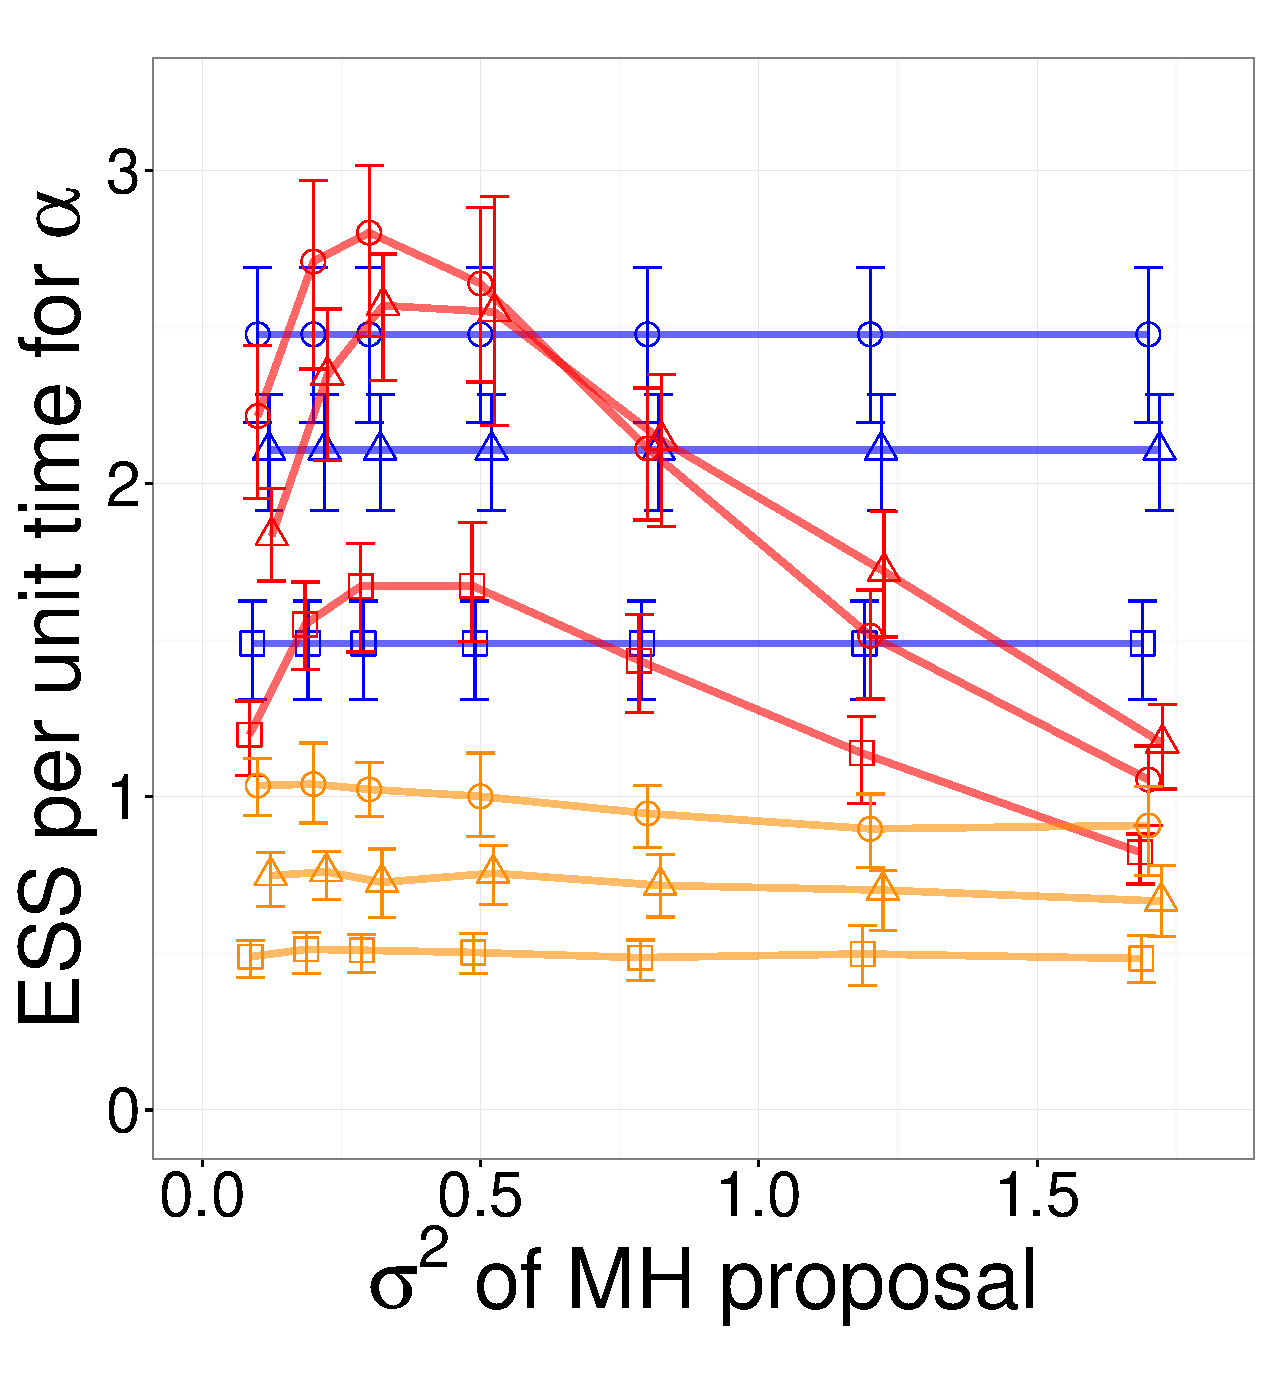
\includegraphics [width=0.90\textwidth, angle=0]{figs/q_5_alpha.pdf}
      \end{minipage}
  \begin{minipage}[hp]{0.45\linewidth}
  \centering
    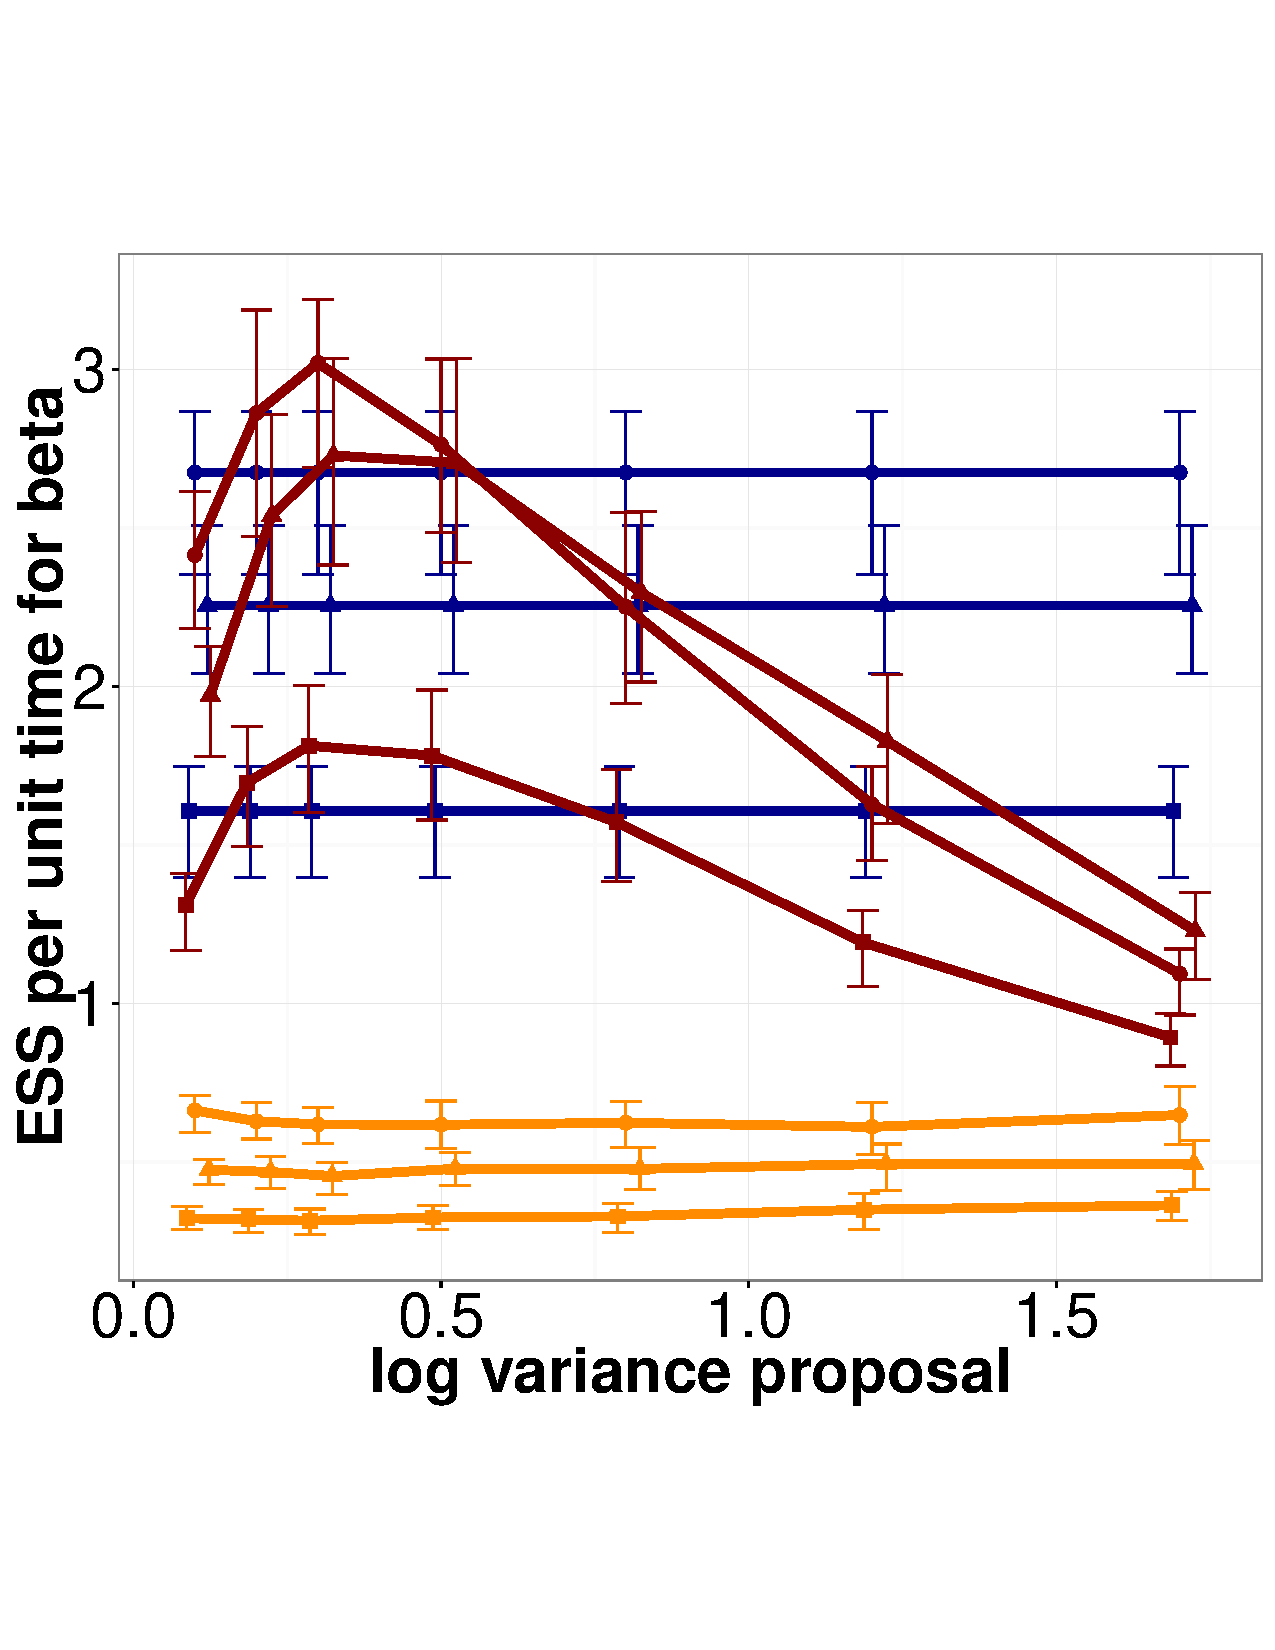
\includegraphics [width=0.90\textwidth, angle=0]{figs/q_5_beta.pdf}
    \vspace{-0 in}
      \label{fig:ESS_Q_D5}
  \end{minipage}
    \caption{ESS/sec for Immigration model (dim 5).The left is for $\alpha$, and the right is for $\beta$.}
  \end{figure}

  \begin{figure}%[b]
  \centering
  \begin{minipage}[!hp]{0.45\linewidth}
  \centering
    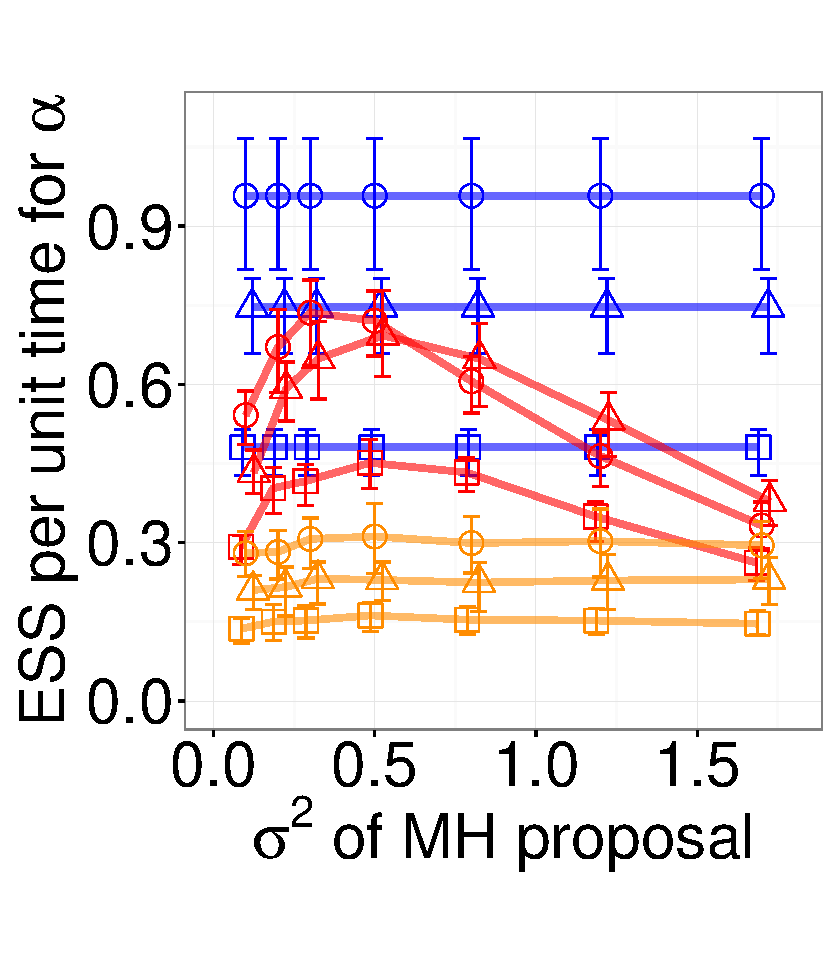
\includegraphics [width=0.90\textwidth, angle=0]{figs/q_10_alpha.pdf}
      \end{minipage}
  \begin{minipage}[hp]{0.45\linewidth}
  \centering
    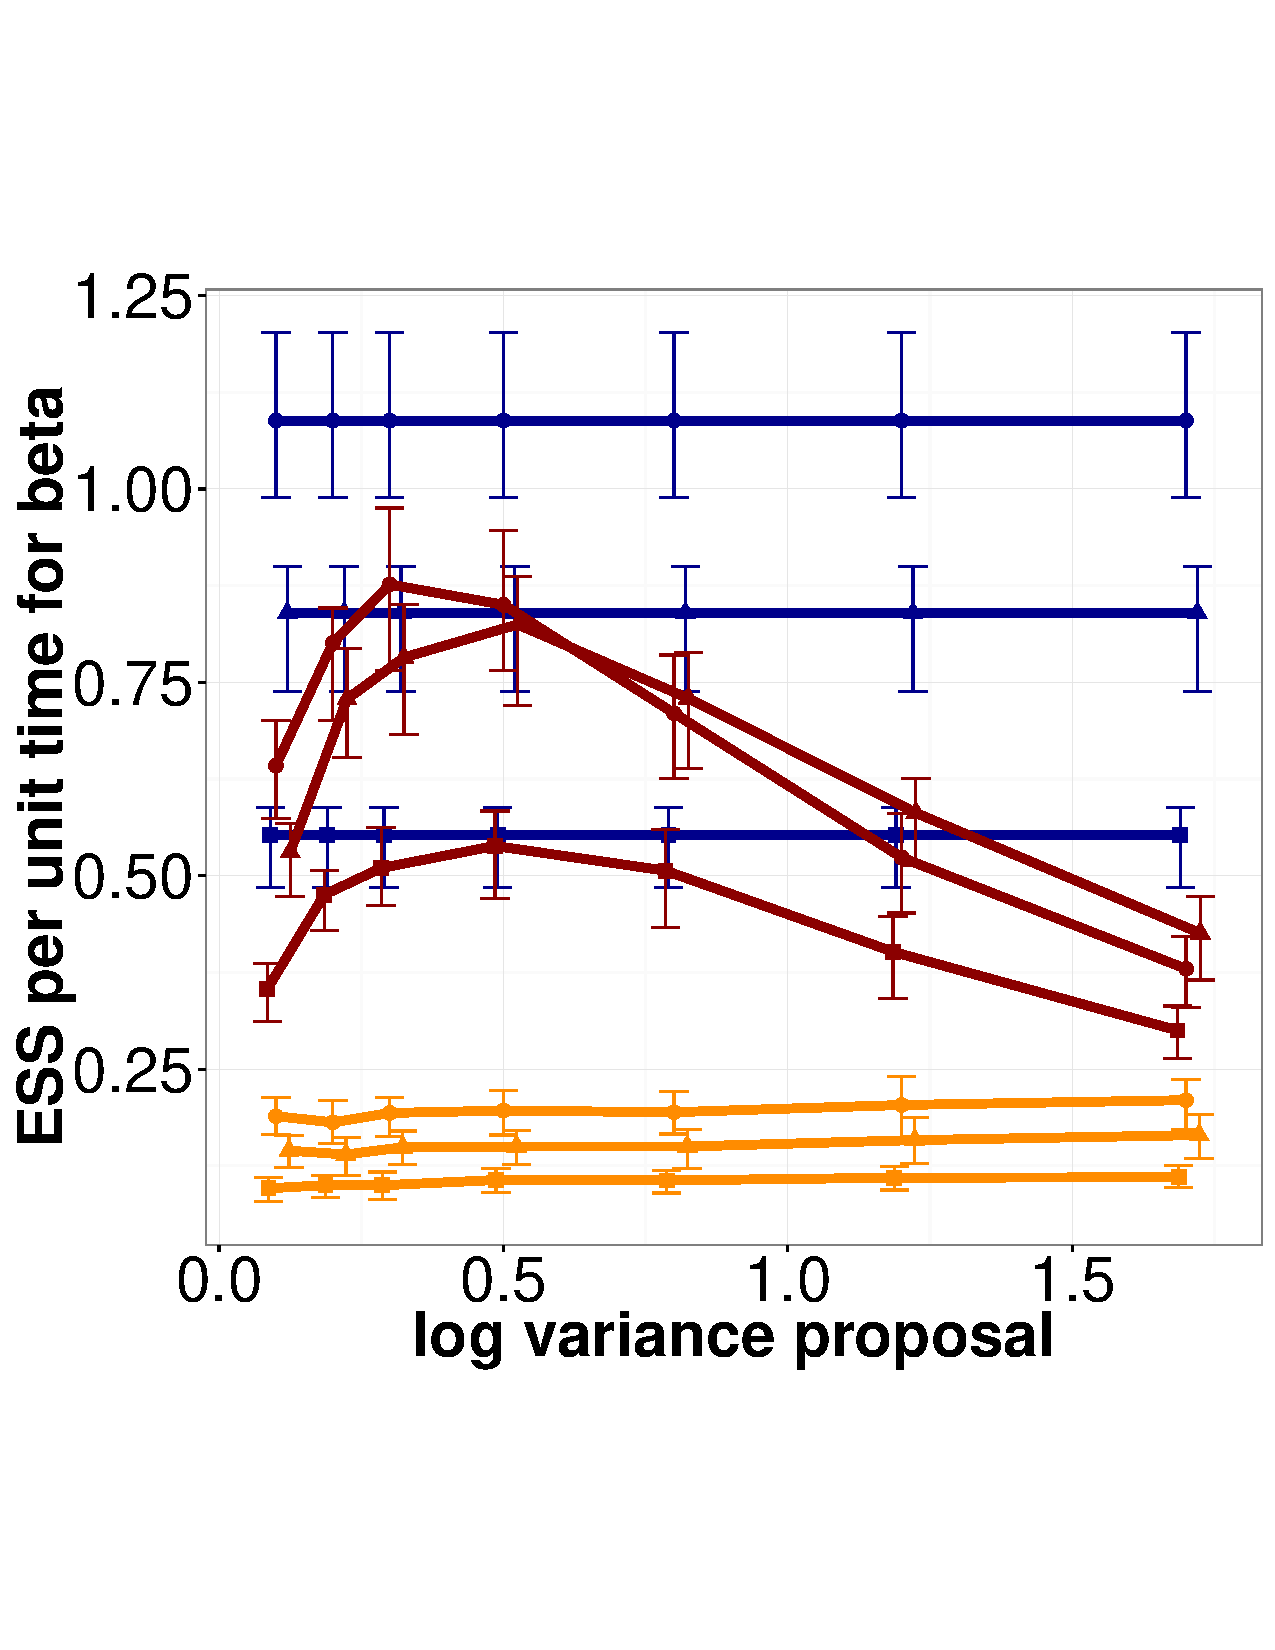
\includegraphics [width=0.90\textwidth, angle=0]{figs/q_10_beta.pdf}
    \vspace{-0 in}
     \label{fig:ESS_Q_D10}
  \end{minipage}
    \caption{ESS/sec for Immigration model (dim 10).The left is for $\alpha$, and the right is for $\beta$.}
  \end{figure}

\begin{figure}
  \begin{minipage}[hp]{0.45\linewidth}
  \centering
    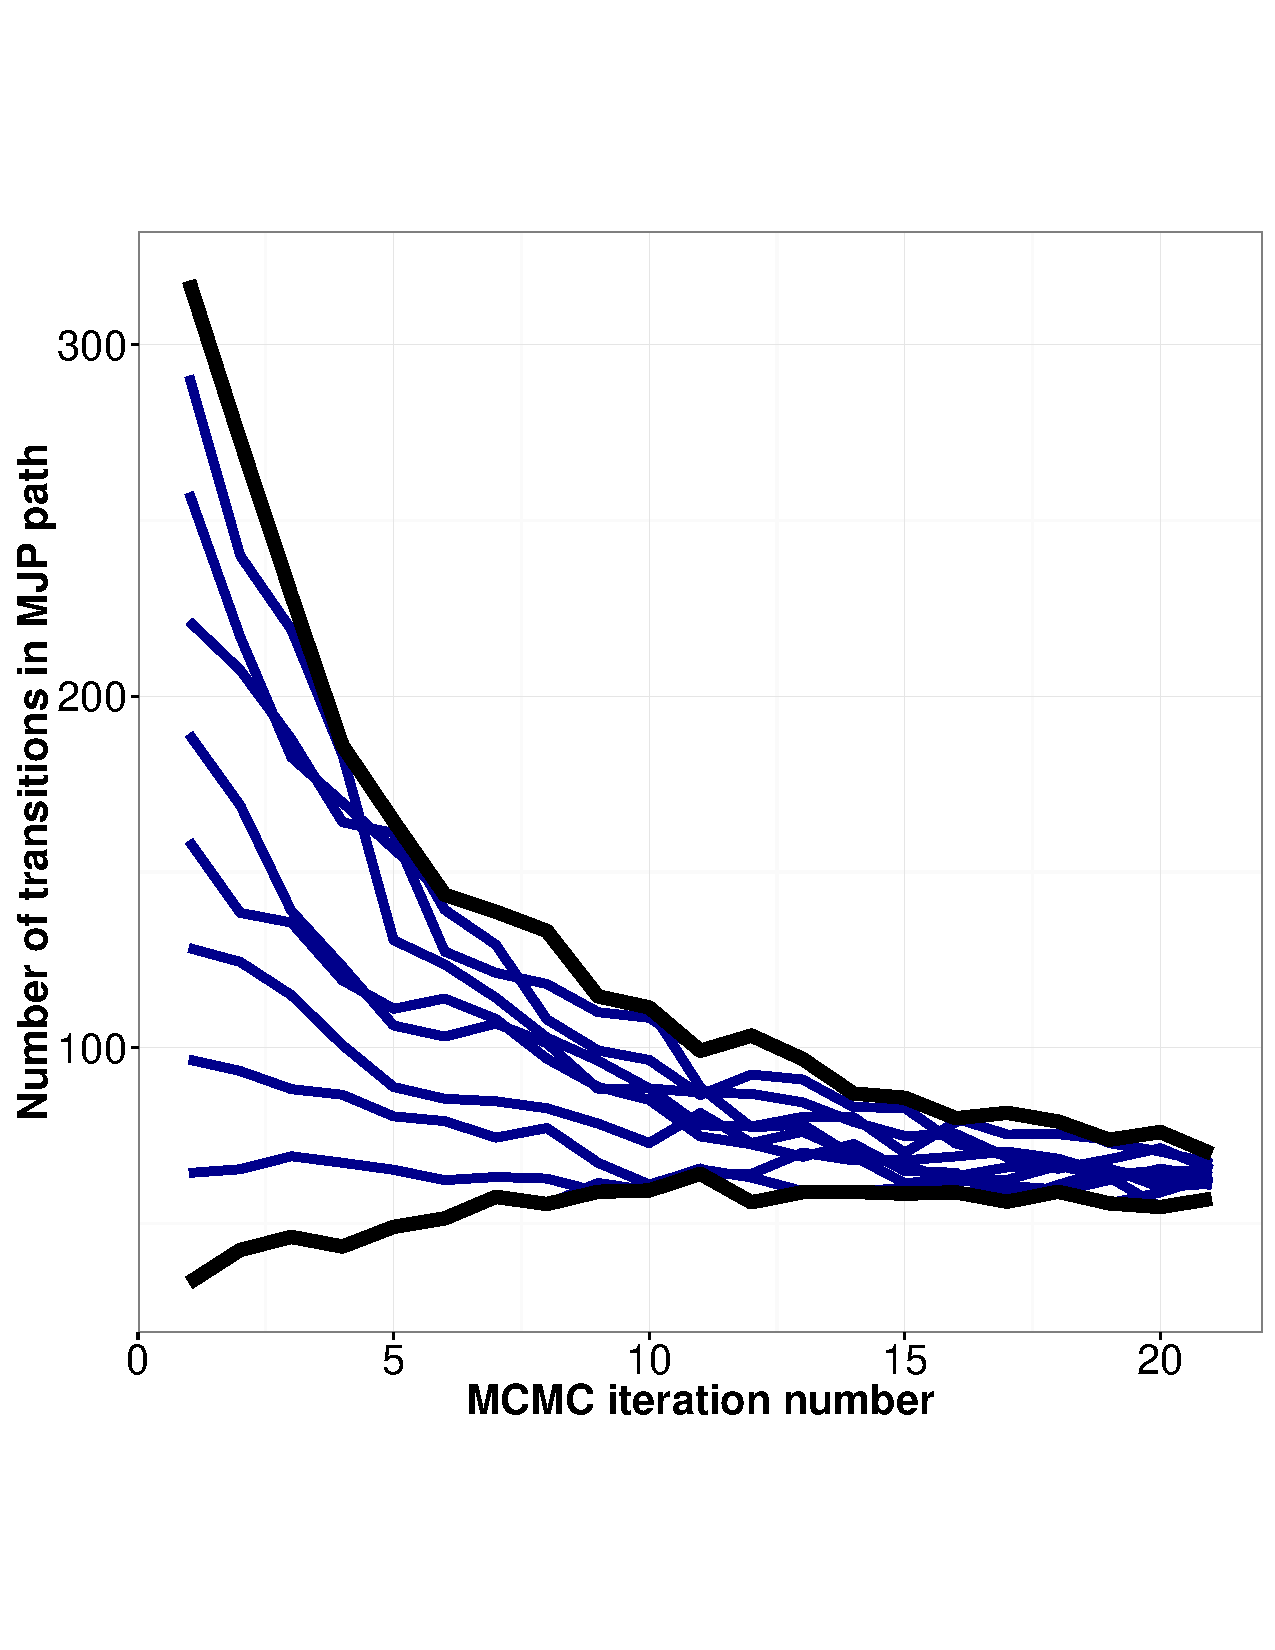
\includegraphics [width=0.90\textwidth, angle=0]{figs/q3_k2_path_transition.pdf}
    \vspace{-0 in}
    \caption{Trace plot of the number of MJP transitions for different initializatoins for immigration model.}
     \label{fig:ESS_Q_TRANSITION}
  \end{minipage}
\end{figure}

  \begin{figure}%[b]
  \begin{minipage}[hp]{0.45\linewidth}
  \centering
    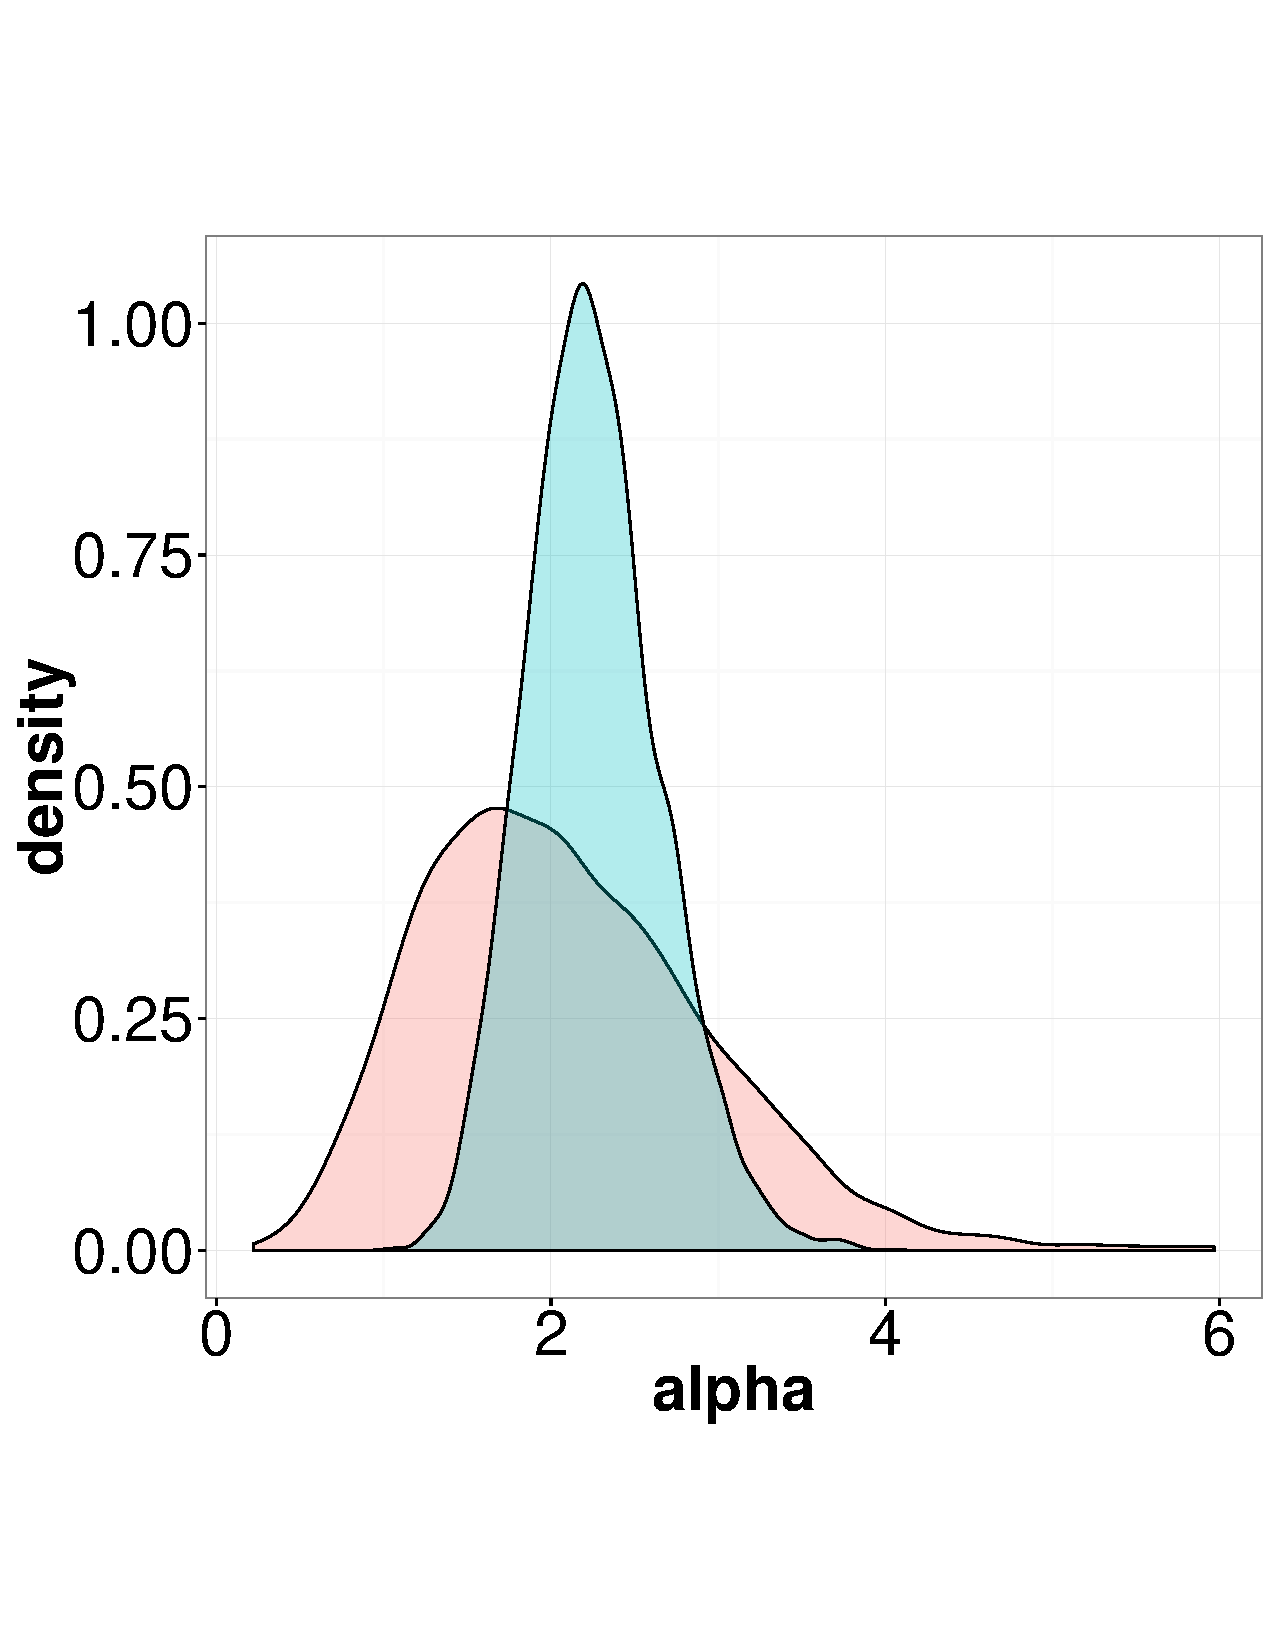
\includegraphics [width=0.90\textwidth, angle=0]{figs/dist_alpha.pdf}
    \vspace{-0 in}
  \end{minipage}
  \begin{minipage}[!hp]{0.45\linewidth}
  \centering
    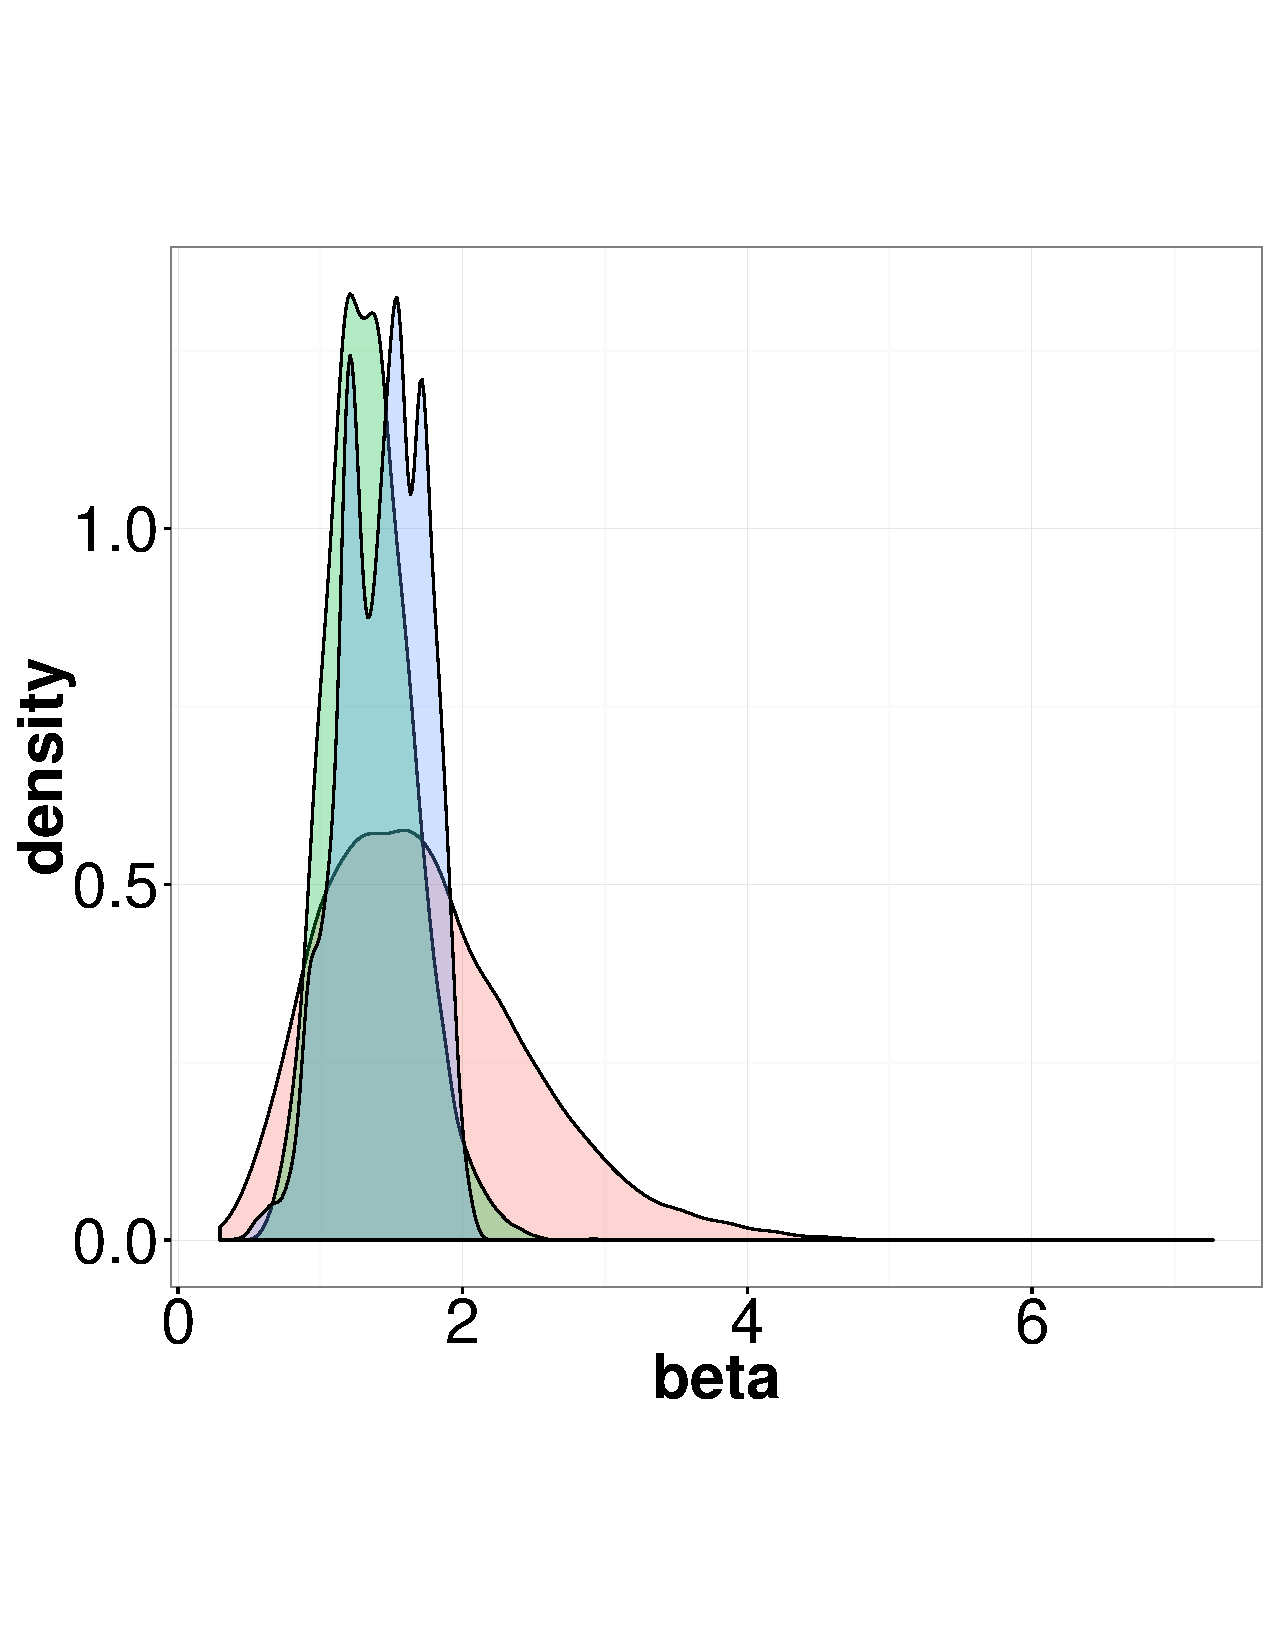
\includegraphics [width=0.90\textwidth, angle=0]{figs/dist_beta.pdf}
    \vspace{-0 in}
  \end{minipage}
    \caption{density.The left is for $\alpha$, and the right is for $\beta$.}
     \label{fig:dist}
  \end{figure}

  \begin{figure}%[b]
  \begin{minipage}[hp]{0.45\linewidth}
  \centering
    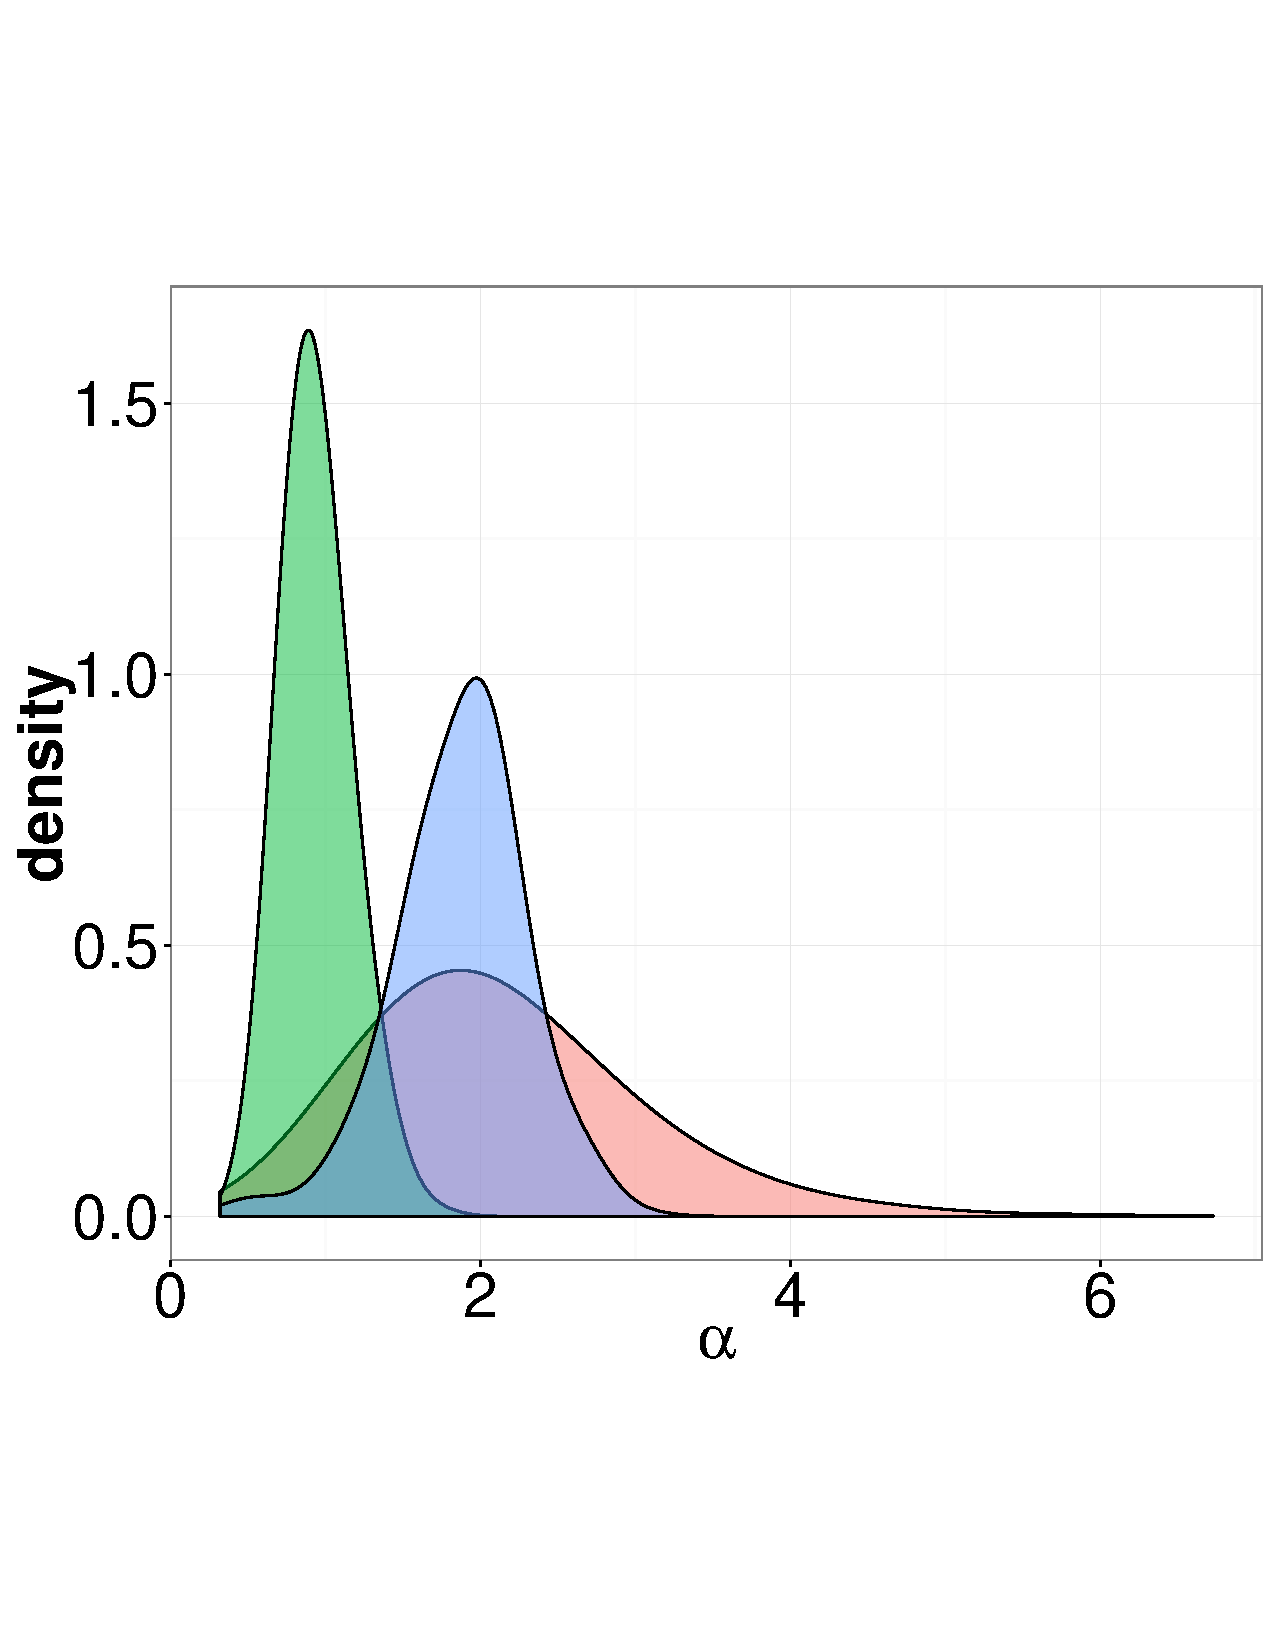
\includegraphics [width=0.90\textwidth, angle=0]{figs/hist_alpha.pdf}
    \vspace{-0 in}
  \end{minipage}
  \begin{minipage}[!hp]{0.45\linewidth}
  \centering
    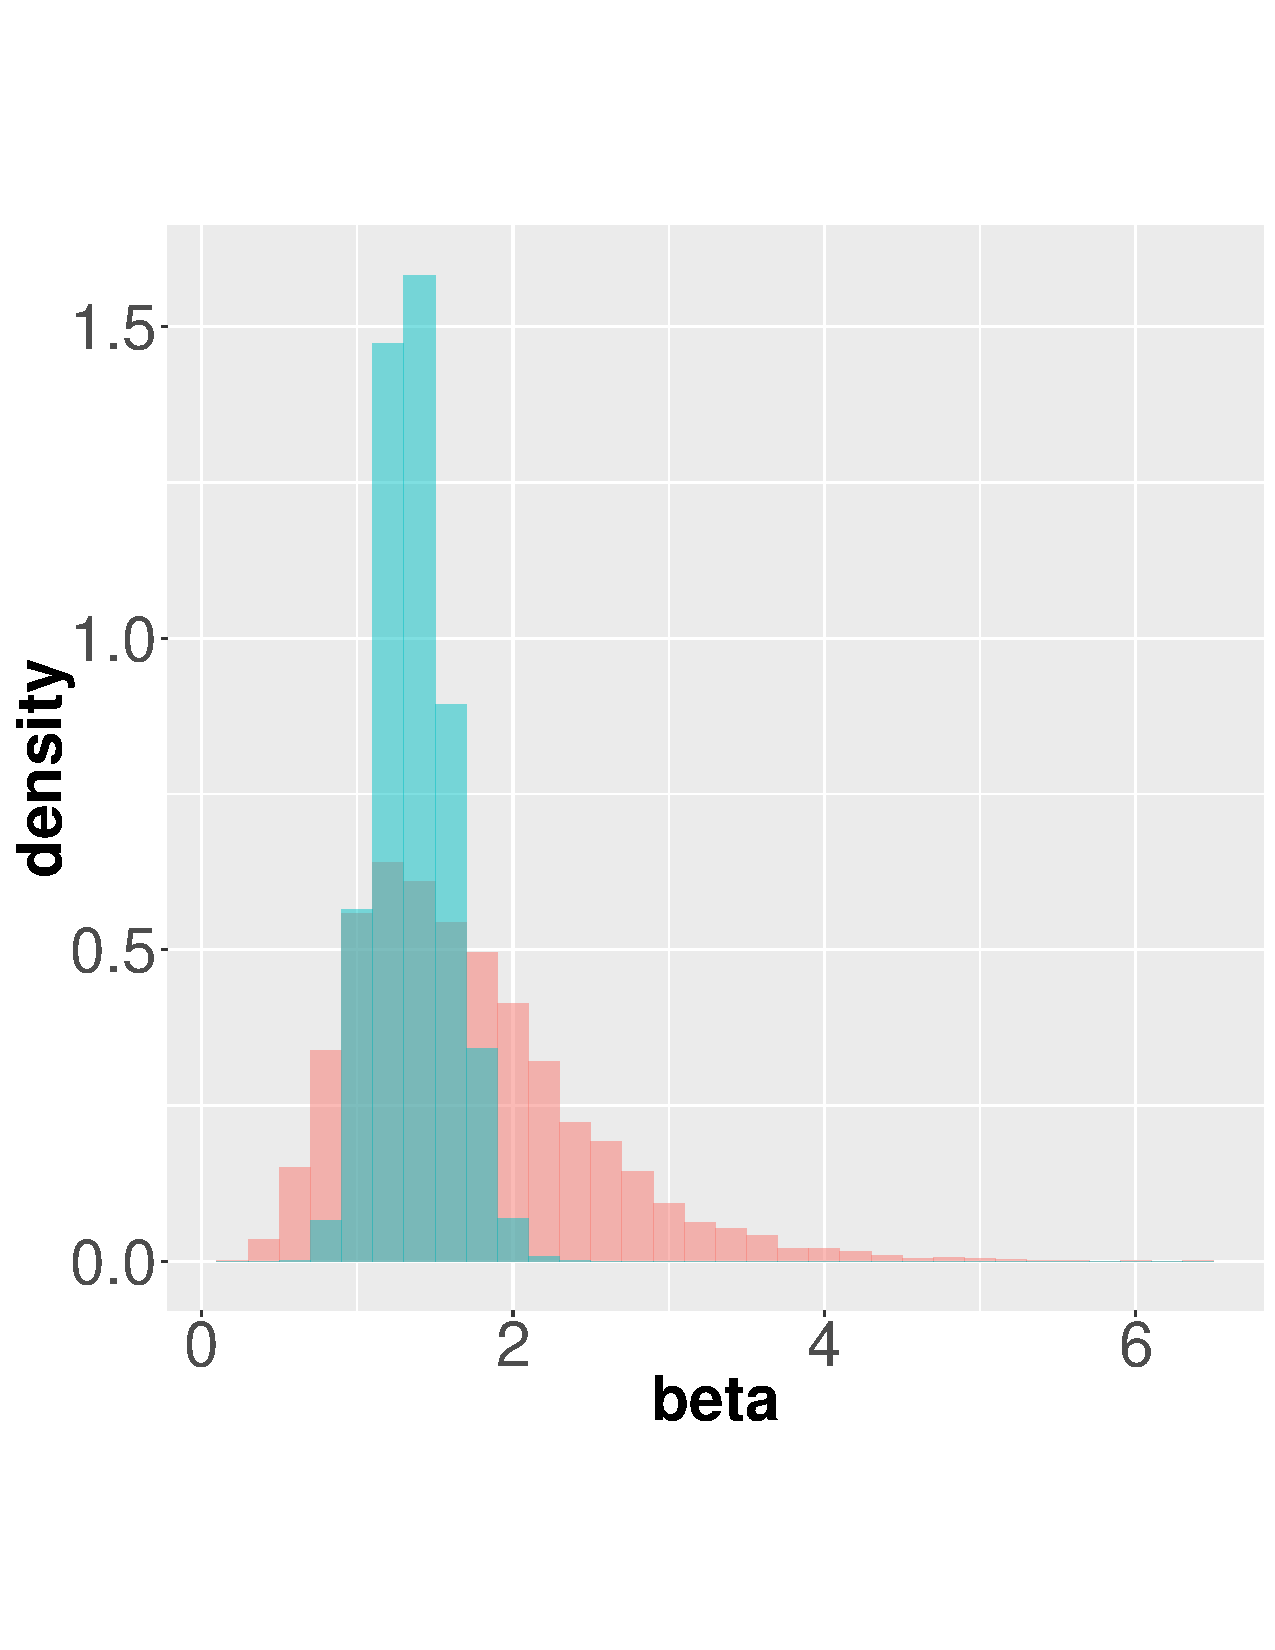
\includegraphics [width=0.90\textwidth, angle=0]{figs/hist_beta.pdf}
    \vspace{-0 in}
  \end{minipage}
    \caption{histogram.The left is for $\alpha$, and the right is for $\beta$.}
     \label{fig:hist}
  \end{figure}
  

\section{DNA evolution JC69 model }~
  \begin{figure}%[H]
  \centering
  \begin{minipage}[!hp]{0.45\linewidth}
  \centering
    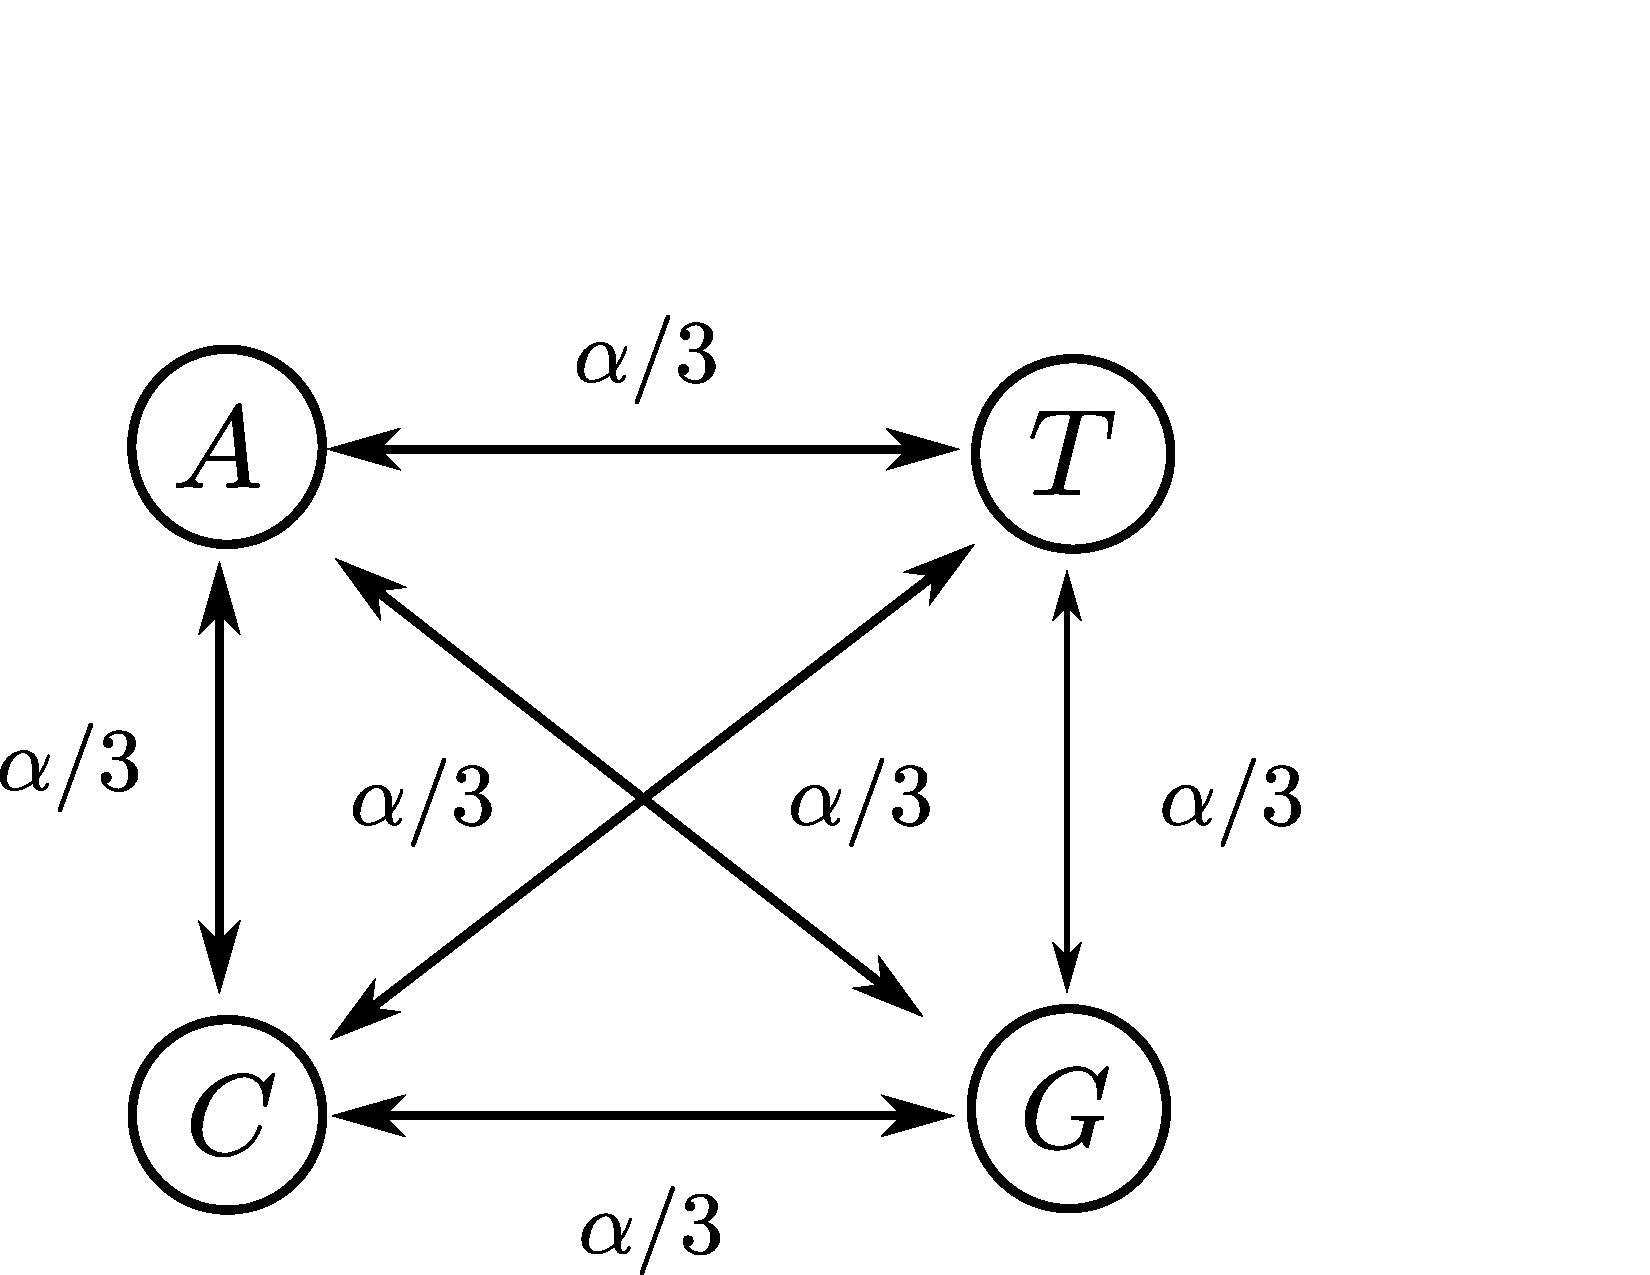
\includegraphics [width=0.90\textwidth, angle=0]{figs/jc_model.pdf}
    \caption{JC69 model}
      \end{minipage}
	\label{jc_model}
  \end{figure}

JC69 is the simplest substitution model. There are several assumptions. It assumes equal base frequencies and equal mutation rates. The only parameter of this model is $\alpha$. The overall substitution rate is therefore $3\alpha$. The state space is $\{0, 1, 2, 3\}$, representing $\{A, T, C, G\}$.\noindent Assume: $S = [S_0,S_1, ...,S_N] \;, T = [t_0(t_{start}), t_1,...,t_N, t_{N+1}(t_{end})]$, and y as observations.\\
$$A_i =: A_{i,i} = -3\alpha, \; \; i =0,1,...,N$$ $$A_{i, j} = \alpha, \; \; i \neq j.$$
If we assume the prior of $\alpha$ is $Gamma(\mu,\lambda)$\\
$$p(\alpha) = \frac{\lambda^\mu}{\Gamma(\mu)}\alpha^{\mu -1}e^{-\lambda \alpha} $$.
Then we can get the posterior distribution $$f(\alpha | s_0,S,T)$$ as follows.
$$ f(\alpha| s_0,S,T) \propto \exp(-(\lambda + 3(t_{end} - t_{start}))\alpha) \alpha^{\mu + N -1} .$$
$\alpha | s_0,S,T$ is following $Gamma(\mu+ N,\lambda + 3(t_{end} - t_{start}))$\\
\section{Experiments}
In the following, we evaluate a Python implementation of our algorithms compared to other exact samplers which include Gibbs sampler and Particle MCMC sampler. We consider three different dimensions which are 3, 5, and 10 and three different k which are 1.5, 2, and 3. We generated random parameters $\alpha$, $\beta$ from prior distributions ($Gamma(3,2), Gamma(5, 2)$), and used this to construct the transition matrix A. Then we generate an MJP trajectory with a uniform initial distribution over states. The state of this MJP trajectory was observed via a Normal distribution with mean equal to the value of state and variance 1, and posterior samples given the observations were produced by a Python implementation of our algorithm. 100 MCMC runs were performed, each run consisting of 10000(Varies among different dimensions) iterations. For each run, the number of transitions as well as the time spent was calculated, and effective sample sizes (ESSs) of these statistics (the number of independent samples with the same `information' as the correlated MCMC samples) were calculated using R-CODA (Plummer et al., 2006). The overall ESS of a run is defined to be the mean ESS across all these ESSs.

\noindent First consider a simple MJP with two parameters $\alpha$ and $\beta$, transitions between states $i$ and $j$ having rate $\alpha /3 $.
We consider three settings for number of states, $3, 5$ and $10$.
Figure~\ref{jc_model}shows the situation with $3$ states.  
We placed Gamma$(\alpha_0,\alpha_1)$, and Gamma$(\beta_0, \beta_1)$ priors on the parameters $\alpha$, $\beta$, with $(\alpha_0,\alpha_1,\beta_0,\beta_1)$ taking
values $(3,2,5,2)$ respectively. In our experiments, we used random parameters drawn from these prior distributions to construct a transition matrix $A$,
and placing a uniform distribution over states at time $0$, sampled an MJP trajectory.
Our observation process was a Gaussian distribution with mean equal to the $\mu_{S_t}$ and variance equal to $1$. $\mu_A = 0$, $\mu_T = 1$, $\mu_C = 2$, $\mu_G = 3$  There are $19$ observations uniformly observed between the time interval $[0, 20]$.

  In Figure~\ref{fig:ESS_JC} we plot the ESS per unit time for the parameters $\alpha$ (left) and $\beta$ (right) as we change the variance of the
  proposal kernel per run, for different methods and different scaling parameters k($k = 1.5, 2, 3$) and different dimensions($p = 3, 5, 10$), where   $k = 1.5$,  $\Omega(\theta, \theta^*) = k \max(\max A(\theta), \max A(\theta^*))$. Blue lines are for Gibbs sampler. Red lines are for improved MH. Orange lines are for naive MH. Black lines are for particle MCMC. Lines with dots correspond to $k = 1.5$. Lines with triangle correspond to $k = 2$. Lines with squares correspond to $k = 3$. For $k=$ $2$ or $3$, $\Omega(\theta, \theta^*) = \frac{k}{2} (\max A(\theta) + \max A(\theta^*))$. We see that the improved MH algorithm is more efficient i	n these cases with respect to the overall ESS per unit time. We also see that increase the scaling parameter will decrease the efficiency of the improved MH algorithm respect to overall ESS per unit time, when $k > 2$. If we set $\Omega = 1.5 \max(\Omega_{old}, \Omega_{new})$, the performance of the improved MH will not be as good as the case we set $\Omega = 2(\Omega_{old} + \Omega_{new})$ when the proposal log variance is large.\\


  \begin{figure}%[b]
  \begin{minipage}[!hp]{0.45\linewidth}
  \centering
    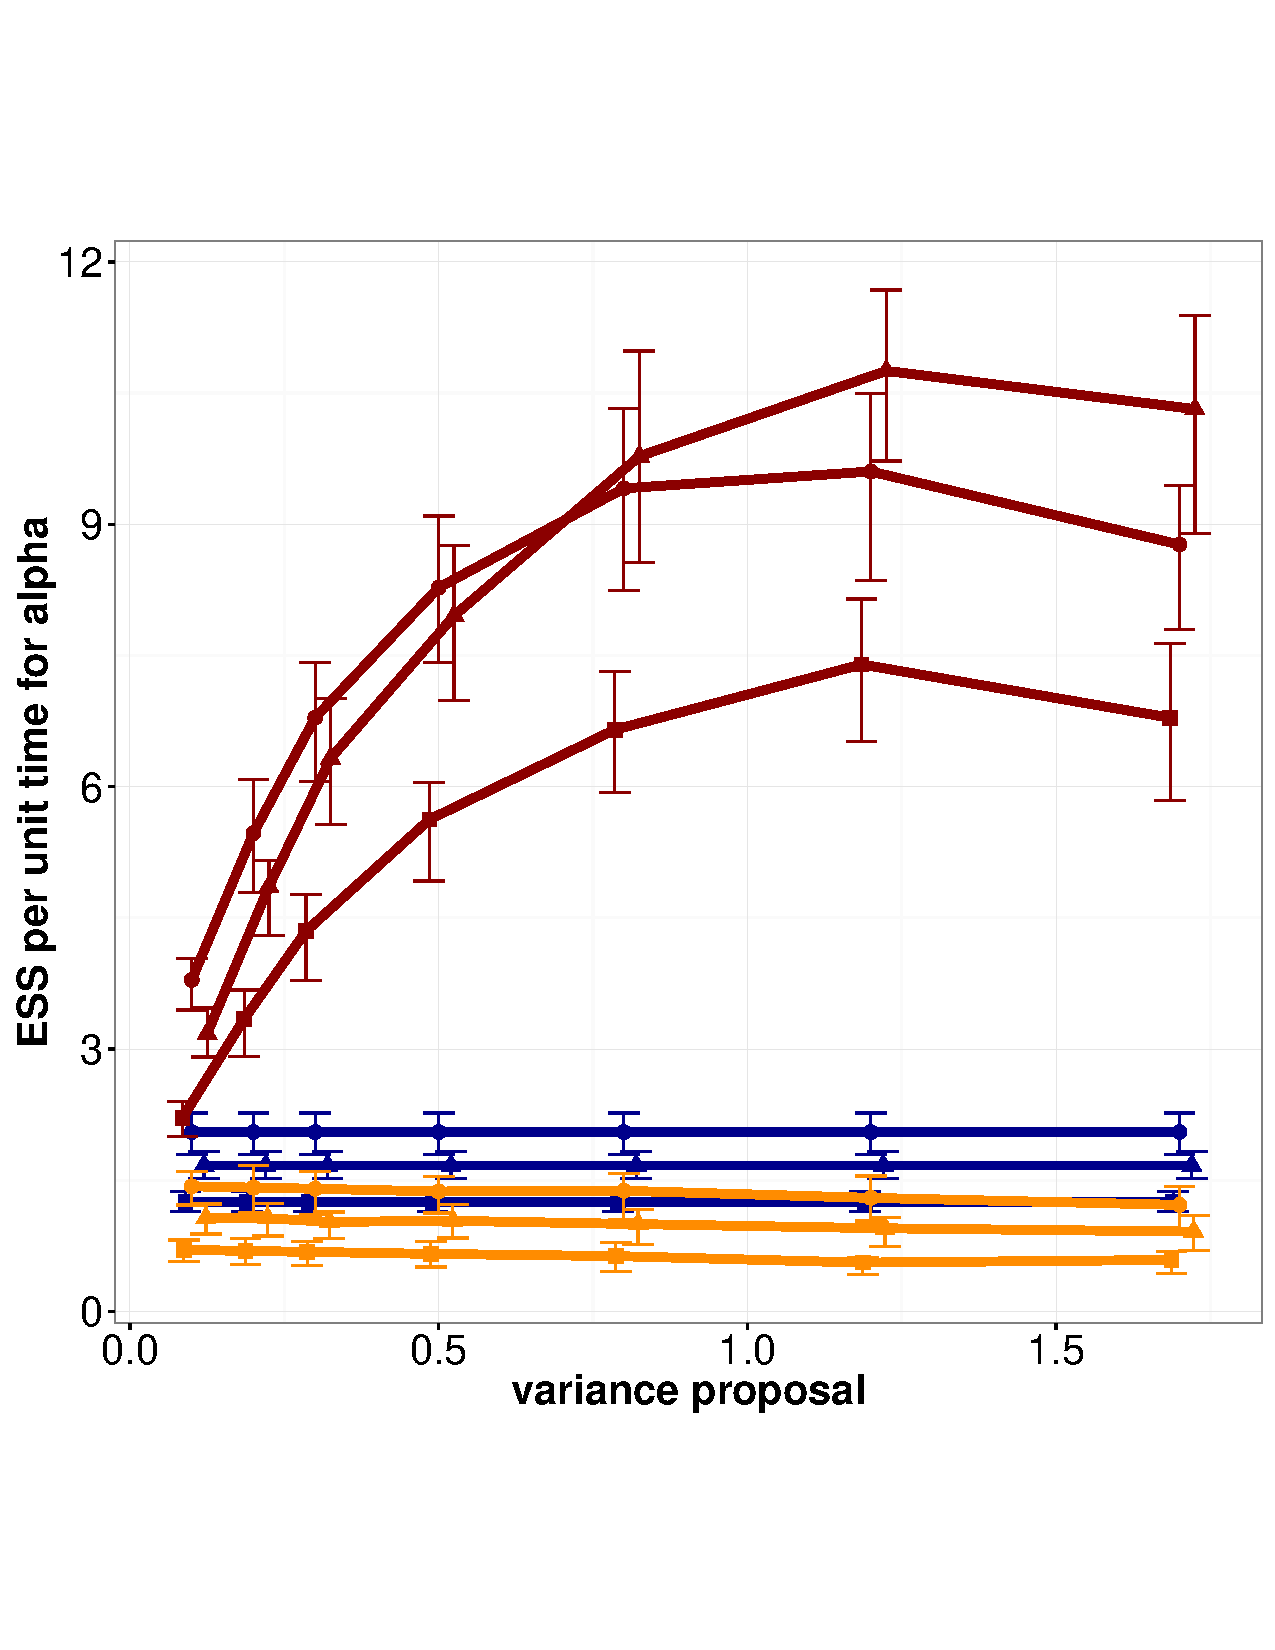
\includegraphics [width=0.70\textwidth, angle=0]{figs/jc.pdf}
    \vspace{-0 in}
    \caption{ESS/sec for JC69 Model }
     \label{fig:ESS_JC}
  \end{minipage}
  \end{figure}



\section{Immigration models with capacity with piece wise constant rate}~
We consider the Queuing model, with piece wise constant transition rate. 
\noindent Assume: $S = [S_0,S_1, ...,S_N] \;, T = [t_0(t_{start}), t_1,...,t_N, t_{N+1}(t_{end})]$, and y as observations.\\
Now, let's consider a immigration model as follows. State space is $\{0, 1, 2, ..., N - 1\}$, representing the total population. The transition matrix is defined as follows. 
$$A_i(t) =: A_{i,i}(t) = -(\alpha + i\beta)w(t), \; \; i =0,1,...,N$$ $$A_{i, i+1}(t) = \alpha w(t), \; \; i =0,1,...,N-1,$$ $$A_{i, i-1}(t)  = \beta w(t), \; \;  i =1,...,N.$$
$w(t)$ is a piece wise constant function. $w(t) = w_i, \; t \in [\l_i, l_{i + 1}), i = 1,2,3,..., K.$\\
We already know the conditional density(given $\alpha,\; \beta$) of a MJP trajectory $(s_0, S, T)$ in time interval $[t_{start}, t_{end}]$, with $S=(s_1, s_2,..., s_k)$, $T=(t_1, t_2,..., t_k)$. 
$$f(s_0,S,T| \alpha, \beta) = \prod_{i=0}^{k-1} A_{s_i, s_{i+1}}(t_i) \exp(\sum_{i=0}^{k} A_{s_i}(t_i)(t_{i+1} - t_{i})), $$
where $t_0 = t_{start}$, $t_{k+1} = t_{end}.$\\
Let's denote some notations here.\\
$$U(s_0, S, T):= \sum_{i=0}^{k-1} \mathbb{I}_{\{s_{i+1} - s_i = 1\}}.$$
$$D(s_0, S, T):= \sum_{i=0}^{k-1} \mathbb{I}_{\{s_{i+1} - s_i = -1\}}.$$
Call them U and D for short.
Let's denote the total time when the trajectory state stays at state i as $\tau_i$, i.e. $\tau_i = \sum_{j=0}^{k} (t_{j+1} -t_j)\mathbb{I}_{\{s_j = i\}}$, then $\sum_{i=0}^k (t_{i+1} - t_i)s_i = \sum_{i=0}^N \tau_ii.$\\

$$f(s_0,S,T| \alpha, \beta) \propto \exp(\sum_{r = 0}^{K}-w_r\alpha(l_{r + 1} - l_{r}- \tau_N^r) )\alpha^U \cdot  \exp(-\int_{t_s}^{t_{e}}(S(t)w(t)\beta)  \beta^D$$\\
If we assume the prior of $\alpha$, and $\beta$ are $Gamma(\mu,\lambda)$, $Gamma(\omega, \theta)$, which are independent with each other. \\
$$p(\alpha) = \frac{\lambda^\mu}{\Gamma(\mu)}\alpha^{\mu -1}e^{-\lambda \alpha}. $$
$$p(\beta) = \frac{\theta^\omega}{\Gamma(\omega)}\beta^{\omega -1}e^{-\theta \beta}. $$
Then we can get the posterior distribution $$f(\alpha, \beta | s_0,S,T)$$ as follows.
$$ f(\alpha, \beta | s_0,S,T) \propto \exp(-(\lambda +\sum_{r = 0}^{K}w_r\alpha(l_{r + 1} - l_{r}- \tau_N^r))\alpha) \alpha^{\mu + U -1} \cdot \exp(-(\int_{t_{s}}^{t_{e}}(S(t)w(t) + \theta)\beta) \beta^{\omega+ D -1}.$$
It means that the posterior distributions of $\alpha$, $\beta$ are still independent. \\
$\alpha | s_0,S,T$ is following $Gamma(\mu+ U,\lambda +\sum_{r = 0}^{K}w_r\alpha(l_{r + 1} - l_{r}- \tau_N^r)  )$\\
$\beta | s_0,S,T$ is following $Gamma(\omega+ D,\int_{t_s}^{t_{e}}(S(t)w(t) + \theta)$.\\
Such immigration models have perfectly conjugate posterior distributions when we assign $\gamma$ priors to $\alpha$ and $\beta$. We apply our Metropolis Hasting algorithms on such models to compare the performance with the performance of Gibbs Sampling algorithm.

\subsection{Experiments}
In the following, we evaluate a Python implementation of our algorithms compared to the Gibbs sampler. We consider three different dimensions which are 3, 5, and 10 and three different k which are 1.5, 2, and 3. We generated random parameters $\alpha$, $\beta$ from prior distributions ($Gamma(3,2), Gamma(5, 2)$). We set $w$ as $(1, 2, 3, 4)$ and $l$ as $(0, 5, 10, 15, 20)$   We used this to construct the transition matrix A. Then we generate an MJP trajectory with a uniform initial distribution over states. The state of this MJP trajectory was observed via a Normal distribution with mean equal to the value of state and variance 1, and posterior samples given the observations were produced by a Python implementation of our algorithm. 100 MCMC runs were performed, each run consisting of 5000(Varies among different dimensions) iterations. For each run, the number of transitions as well as the time spent was calculated, and effective sample sizes (ESSs) of these statistics (the number of independent samples with the same `information' as the correlated MCMC samples) were calculated using R-CODA (Plummer et al., 2006). The overall ESS of a run is defined to be the mean ESS across all these ESSs.

 In Figure~\ref{fig:ESS_pc_3}, Figure~\ref{fig:ESS_pc_5}, Figure~\ref{fig:ESS_pc_10}, we plot the ESS per unit time for the parameters $\alpha$ (left) and $\beta$ (right) as we change the variance of the
  proposal kernel per run, for different methods and different scaling parameters k($k = 1.5, 2, 3$) and different dimensions($p = 3, 5, 10$), where   $k = 1.5$,  $\Omega(\theta, \theta^*) = k \max(\max A(\theta), \max A(\theta^*))$. Blue lines are for Gibbs sampler. Red lines are for improved MH. Orange lines are for naive MH. Black lines are for particle MCMC. Lines with dots correspond to $k = 1.5$. Lines with triangle correspond to $k = 2$. Lines with squares correspond to $k = 3$. For $k=$ $2$ or $3$, $\Omega(\theta, \theta^*) = \frac{k}{2} (\max A(\theta) + \max A(\theta^*))$. We see that the improved MH algorithm is more efficient i	n these cases with respect to the overall ESS per unit time. We also see that increase the scaling parameter will decrease the efficiency of the improved MH algorithm respect to overall ESS per unit time, when $k > 2$. If we set $\Omega = 1.5 \max(\Omega_{old}, \Omega_{new})$, the performance of the improved MH will not be as good as the case we set $\Omega = 2(\Omega_{old} + \Omega_{new})$ when the proposal log variance is large.\\

  \begin{figure}%[b]
  \centering
  \begin{minipage}[!hp]{0.45\linewidth}
  \centering
    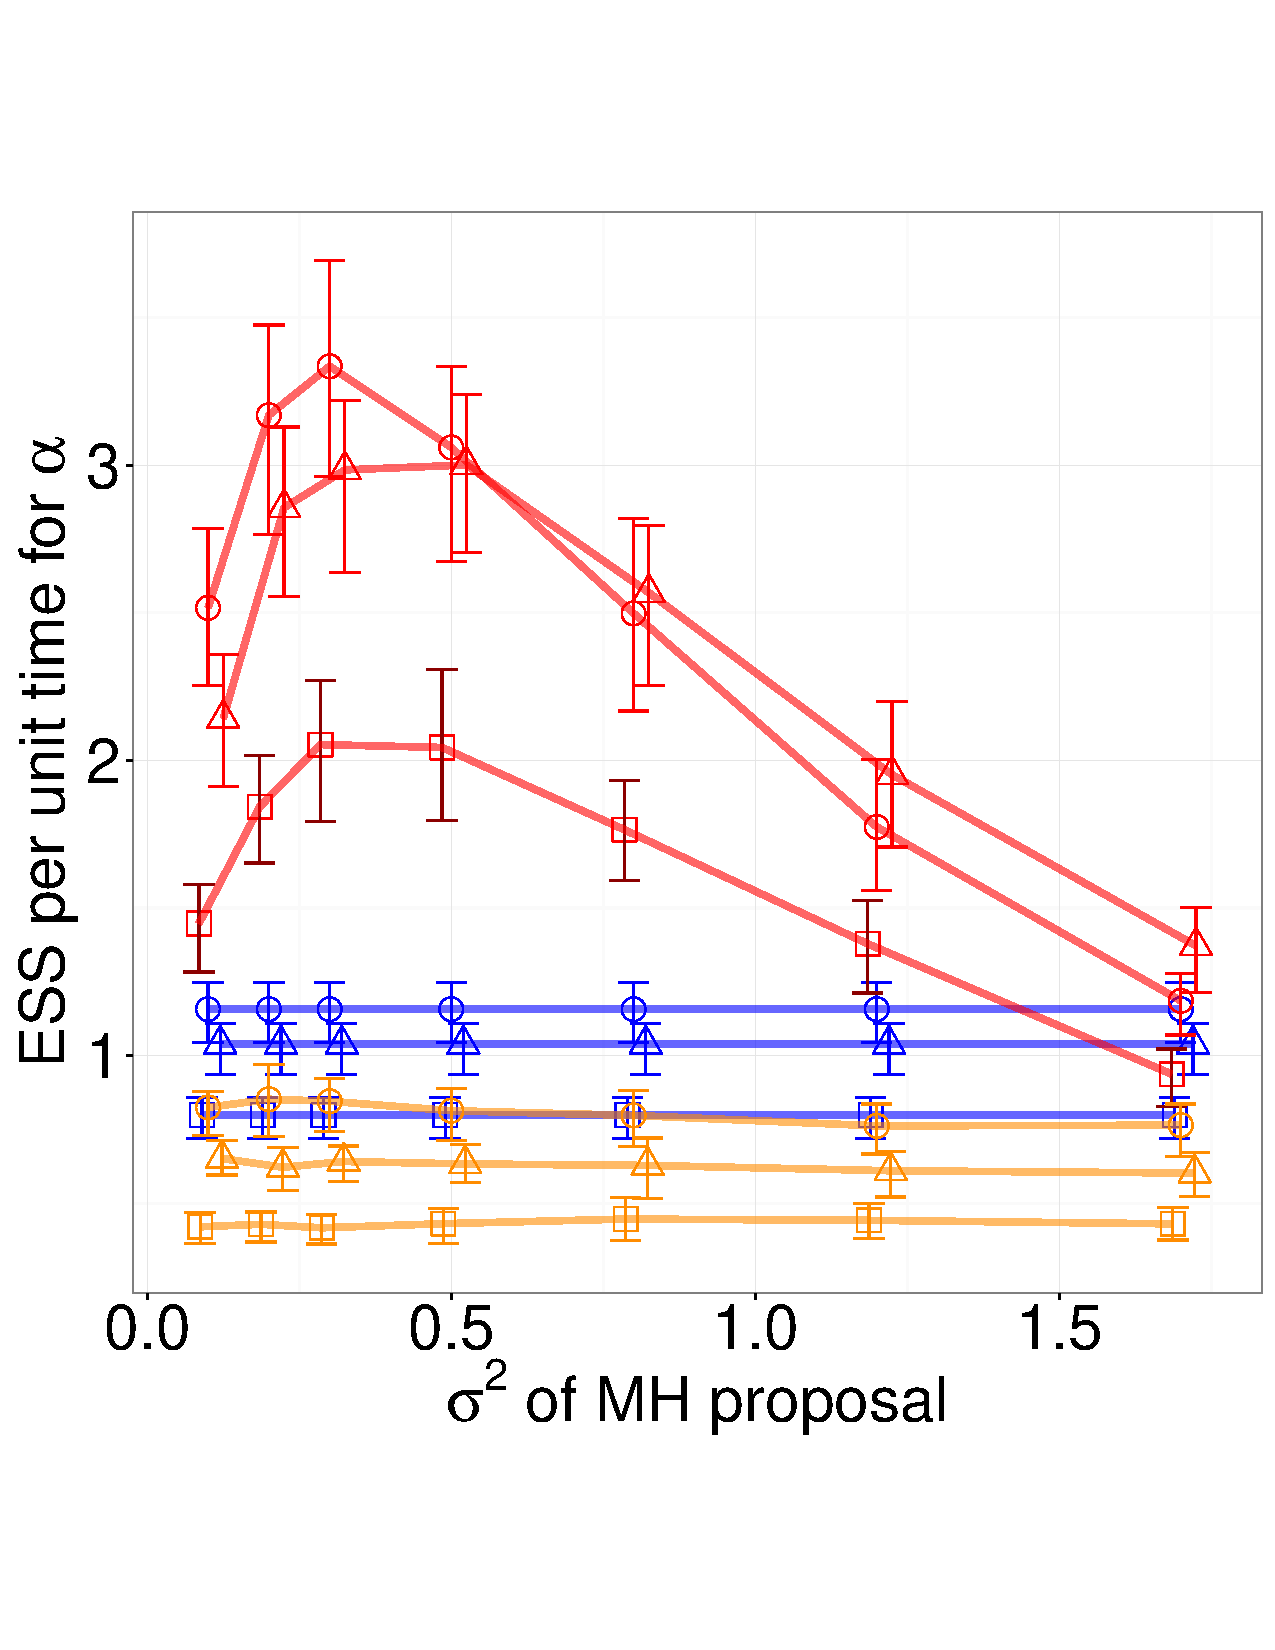
\includegraphics [width=0.70\textwidth, angle=0]{figs/pc_3_alpha.pdf}
      \end{minipage}
  \begin{minipage}[!hp]{0.45\linewidth}
  \centering
    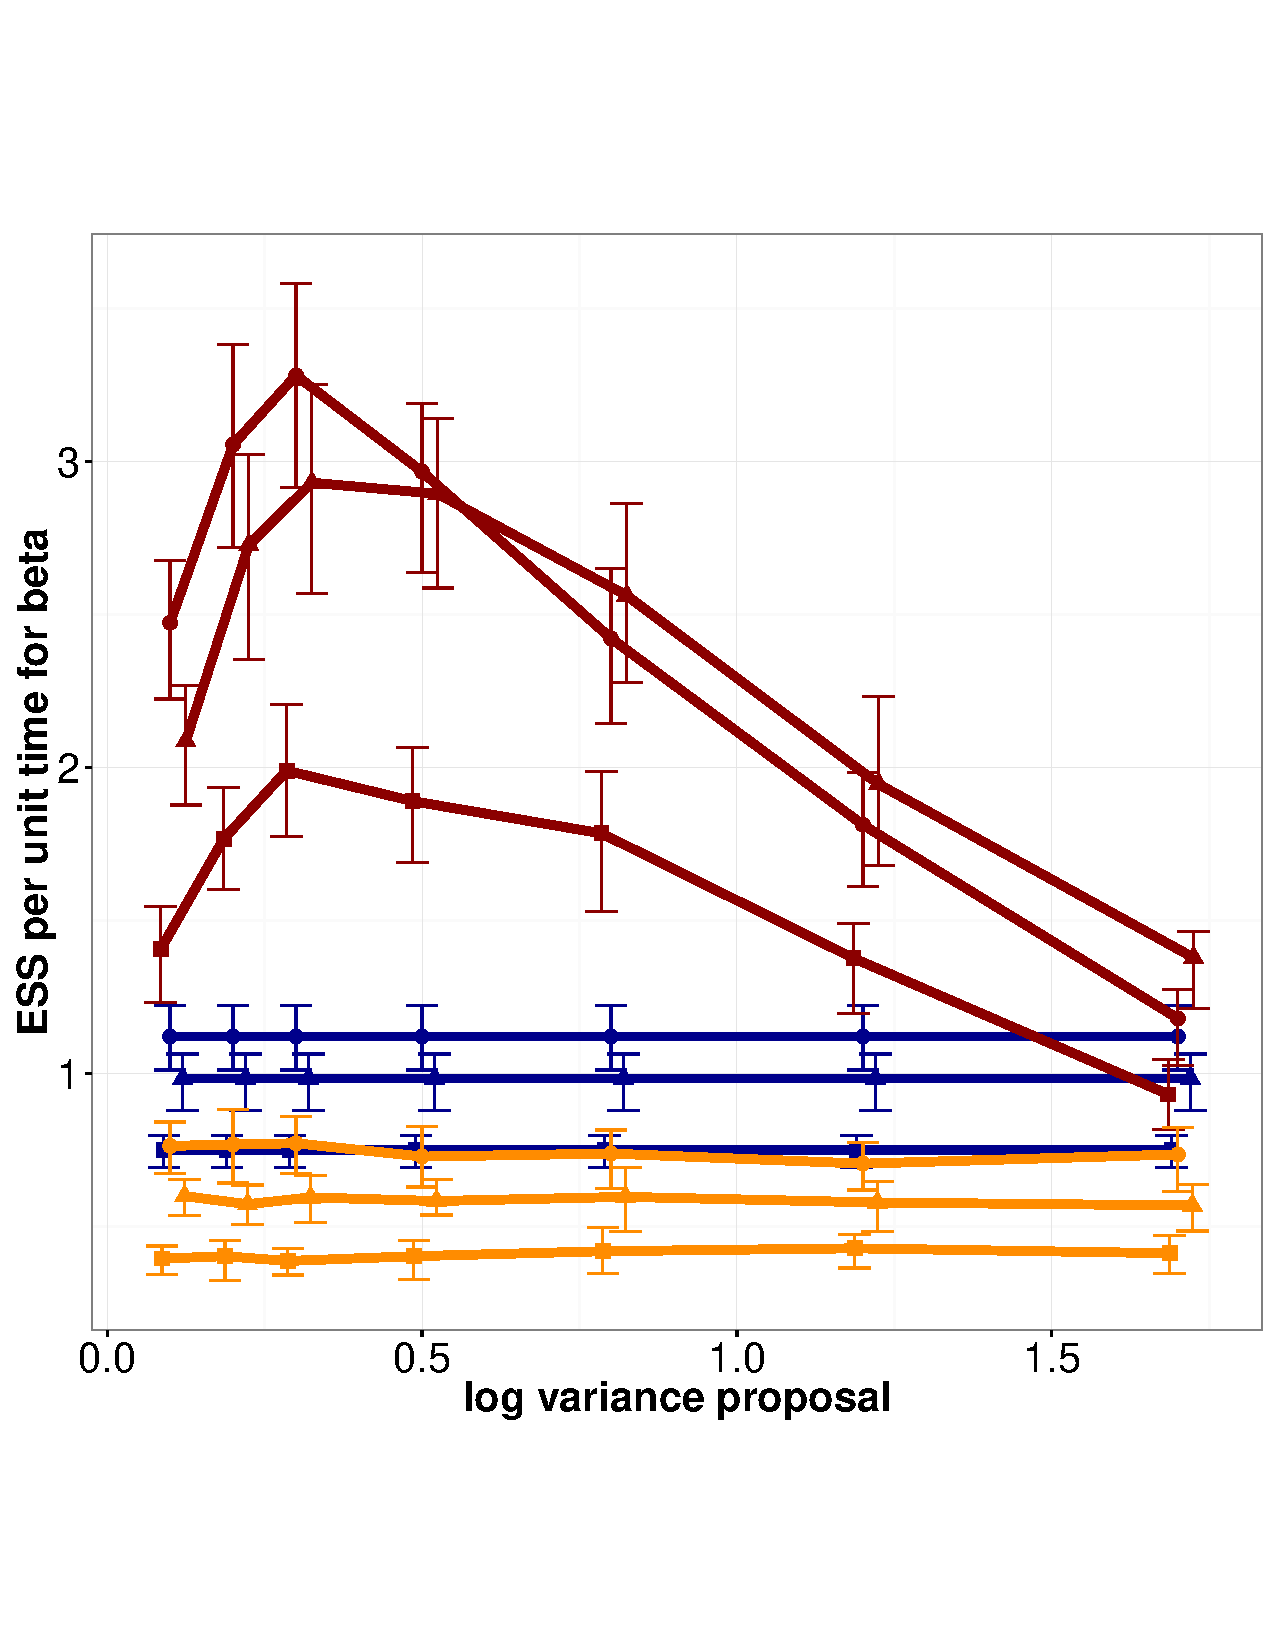
\includegraphics [width=0.70\textwidth, angle=0]{figs/pc_3_beta.pdf}
    \vspace{-0 in}
     \label{fig:ESS_pc_3}
  \end{minipage}
    \caption{ESS/sec for NH Immigration model (dim 3)}
  \end{figure}
  \begin{figure}%[b]
  \centering
  \begin{minipage}[!hp]{0.45\linewidth}
  \centering
    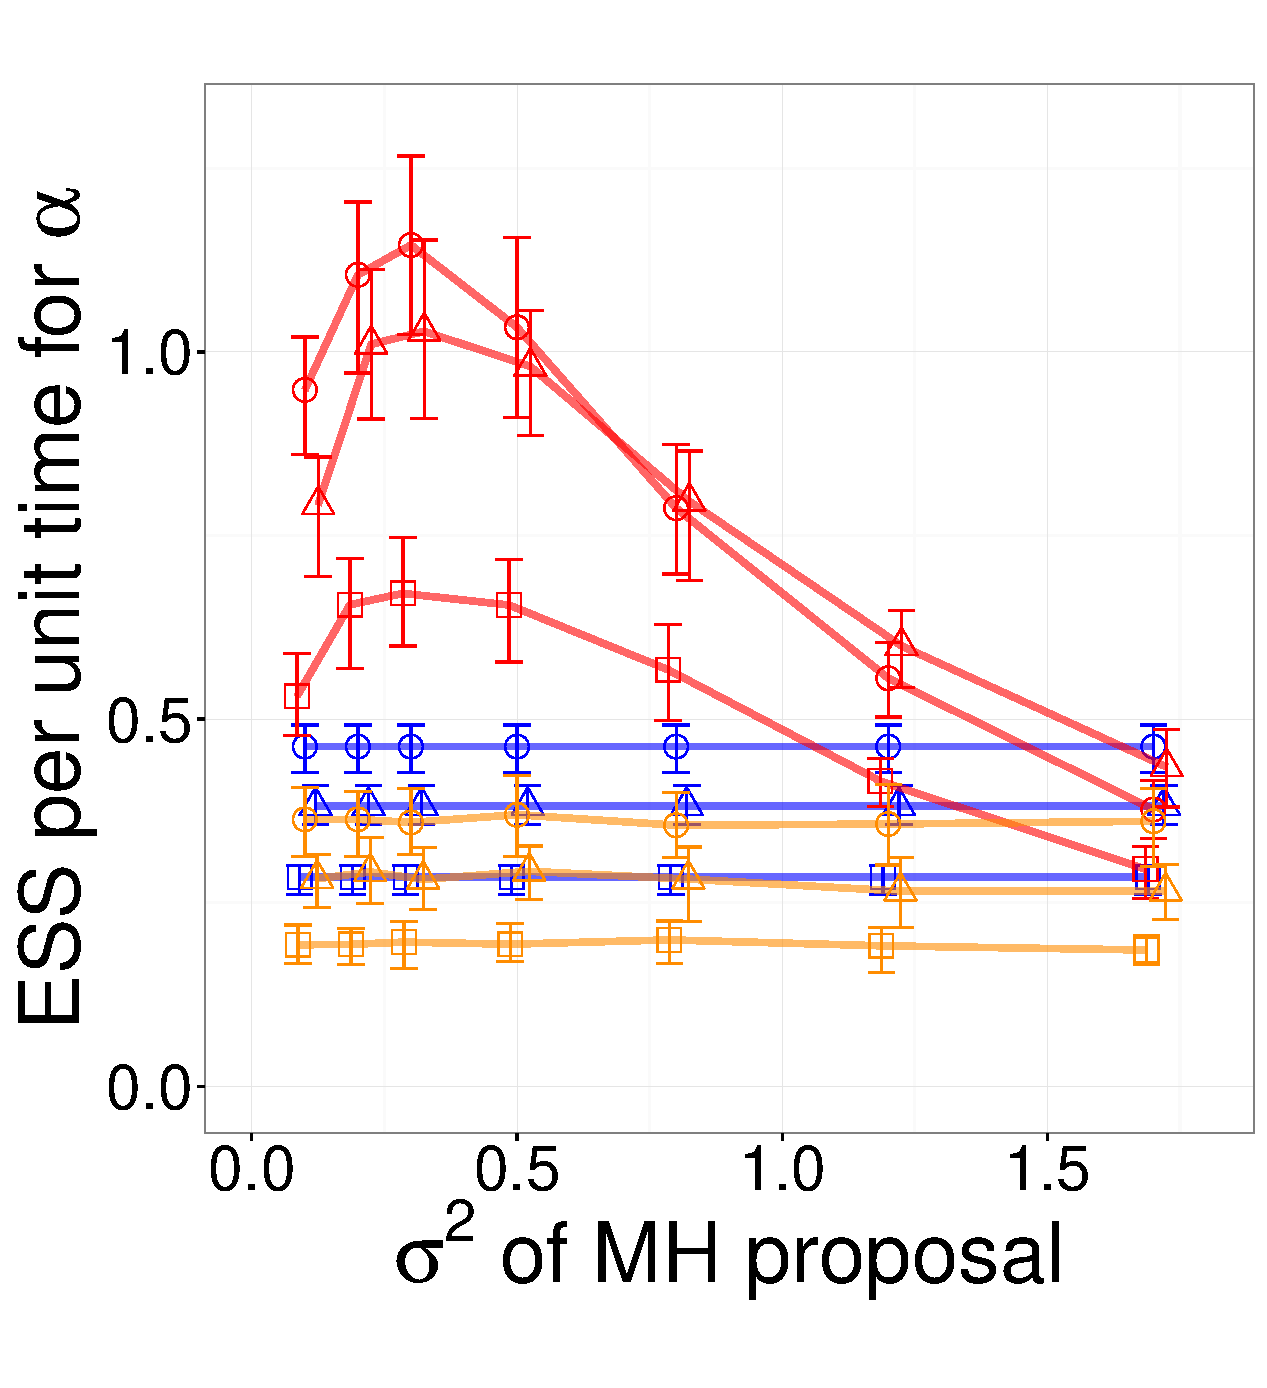
\includegraphics [width=0.70\textwidth, angle=0]{figs/pc_5_alpha.pdf}
      \end{minipage}
  \begin{minipage}[!hp]{0.45\linewidth}
  \centering
    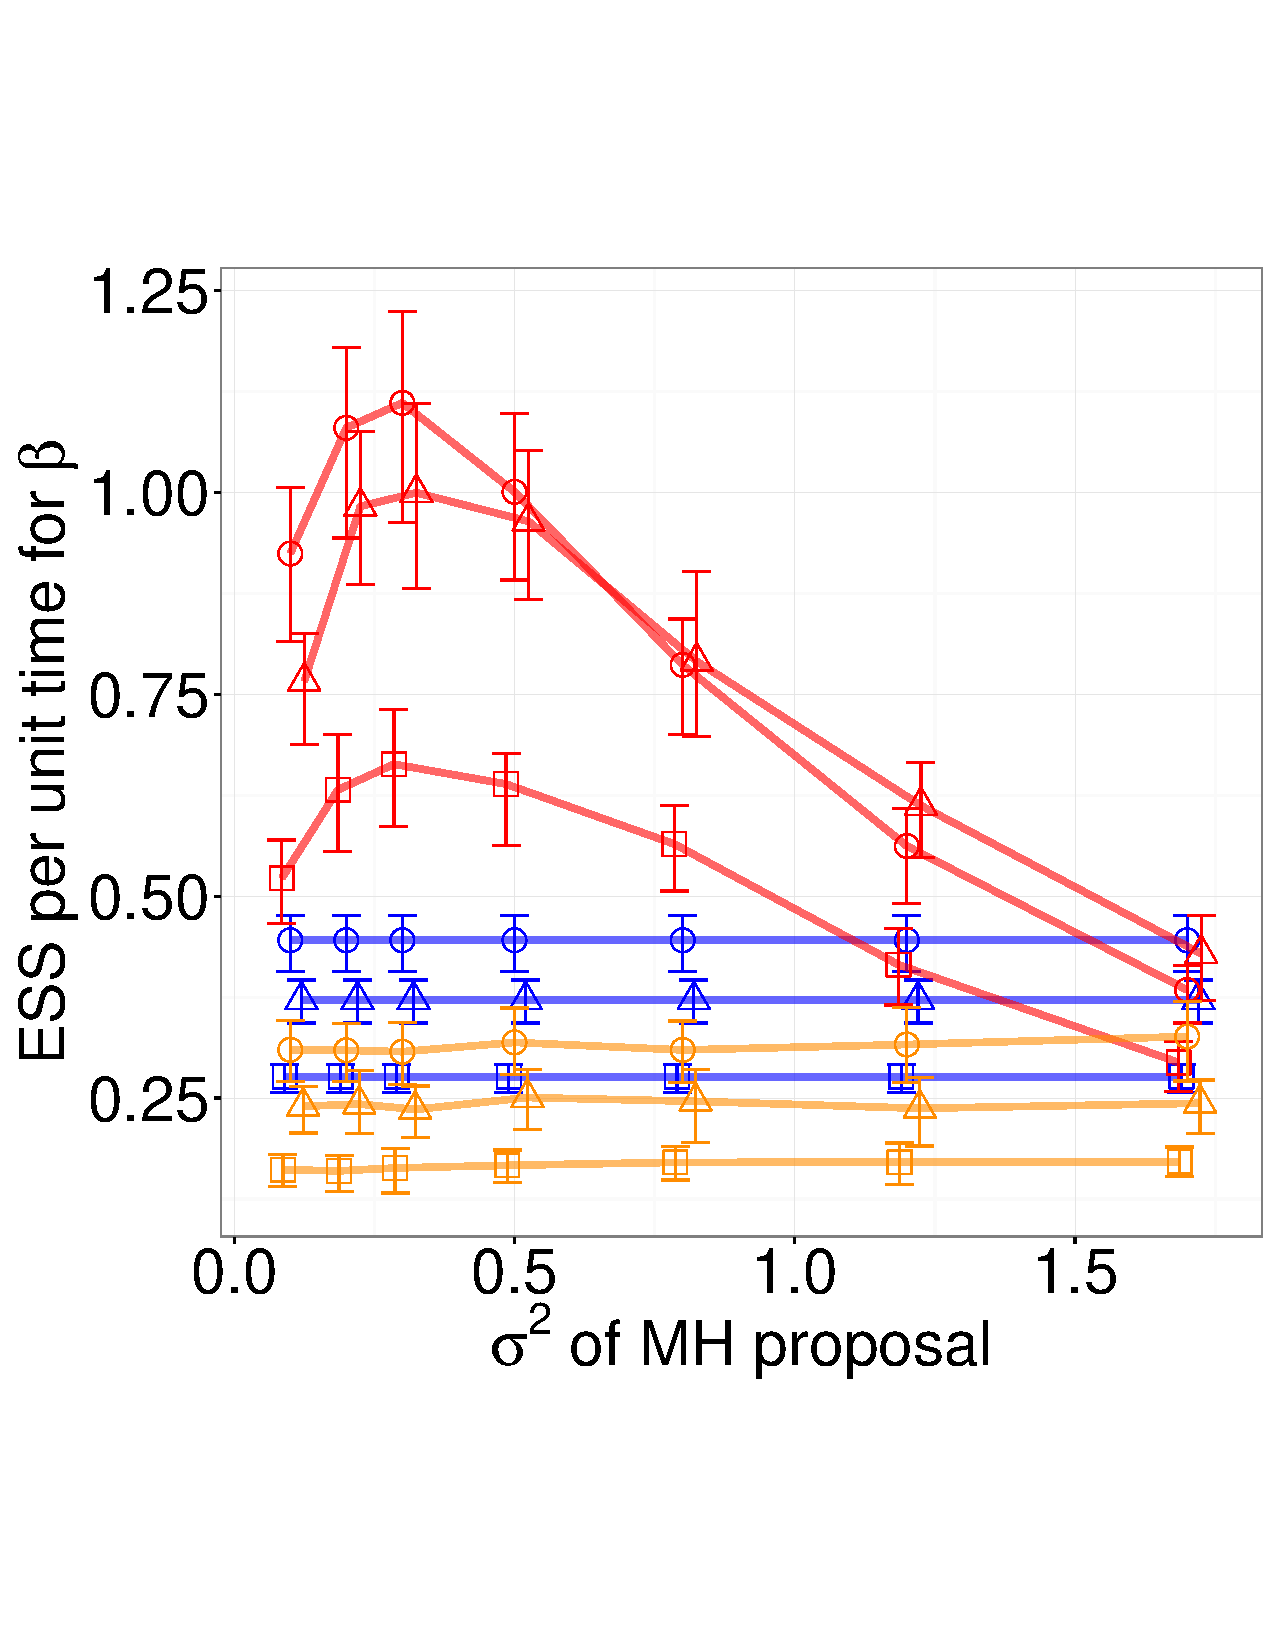
\includegraphics [width=0.70\textwidth, angle=0]{figs/pc_5_beta.pdf}
    \vspace{-0 in}
     \label{fig:ESS_pc_5}
  \end{minipage}
    \caption{ESS/sec for NH Immigration model (dim 5)}
  \end{figure}

  \begin{figure}%[b]
  \centering
  \begin{minipage}[!hp]{0.45\linewidth}
  \centering
    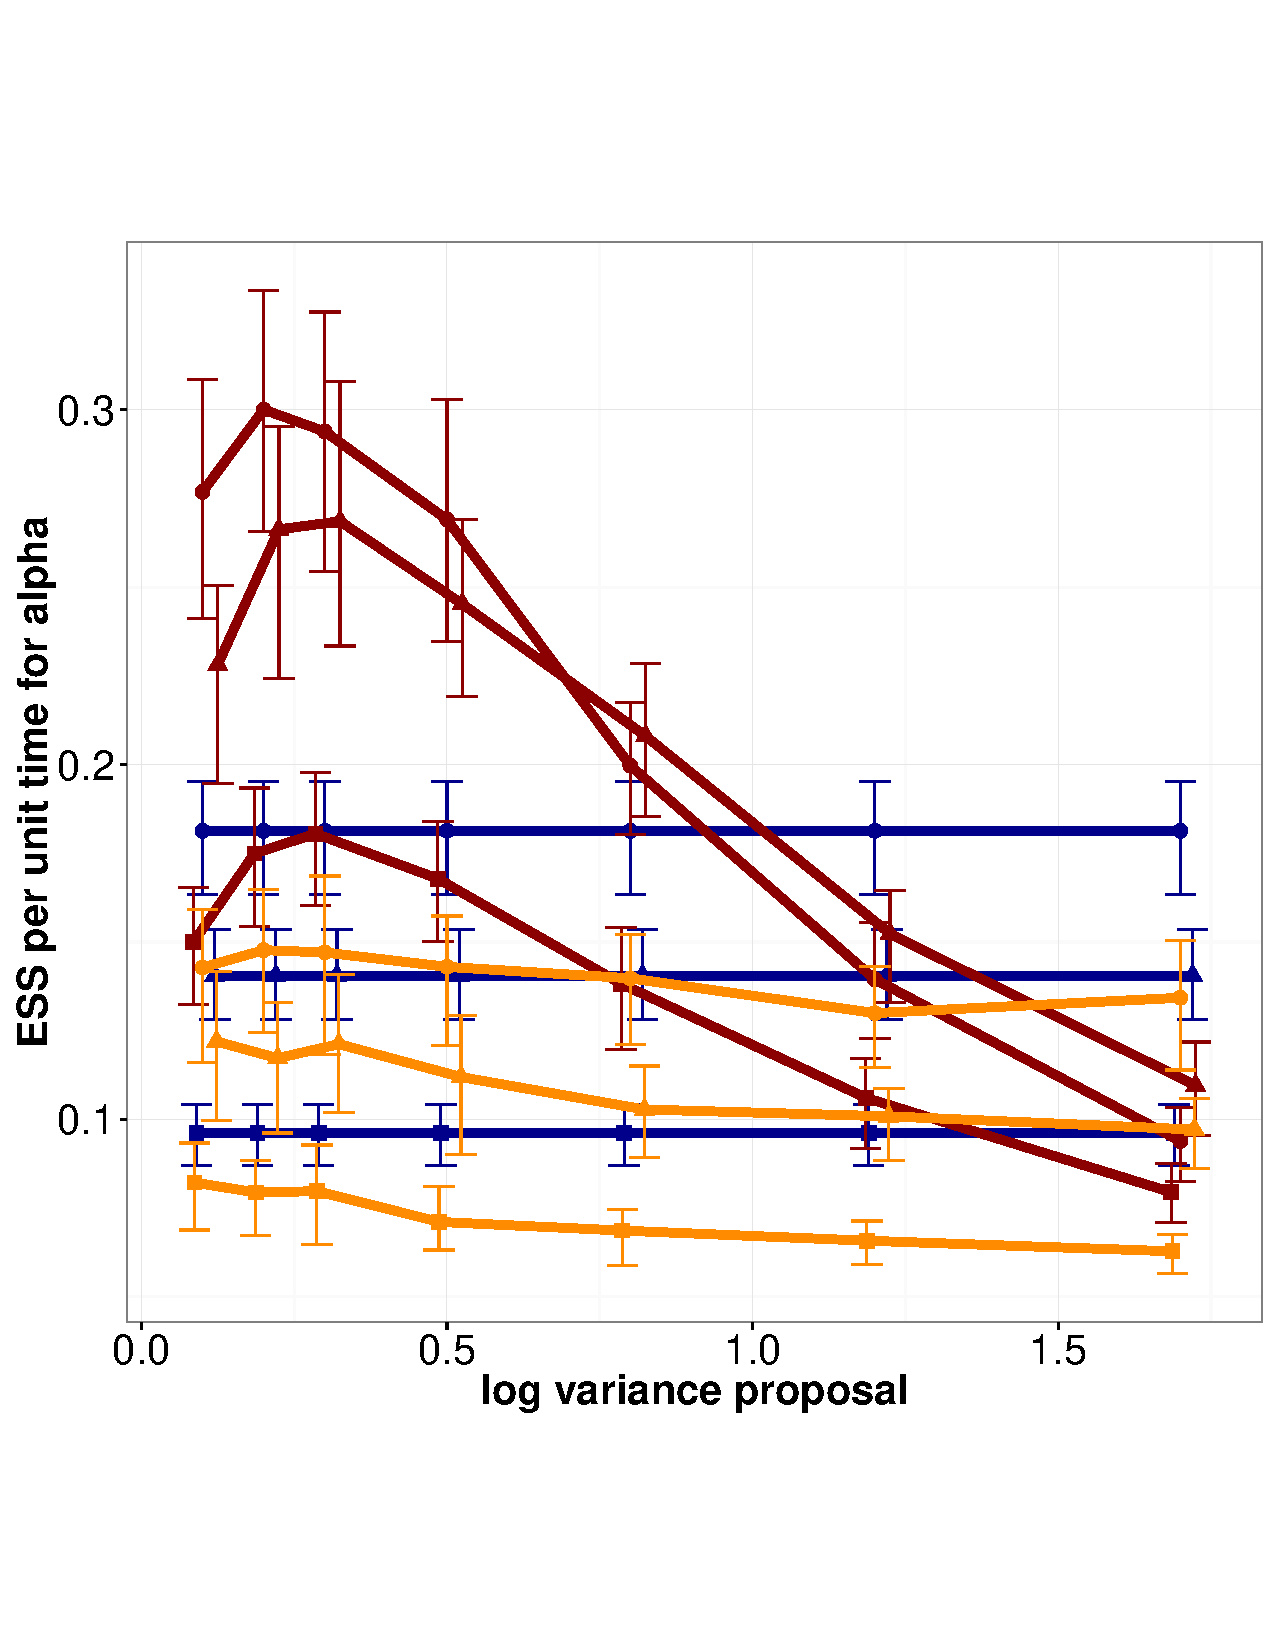
\includegraphics [width=0.70\textwidth, angle=0]{figs/pc_10_alpha.pdf}
      \end{minipage}
  \begin{minipage}[!hp]{0.45\linewidth}
  \centering
    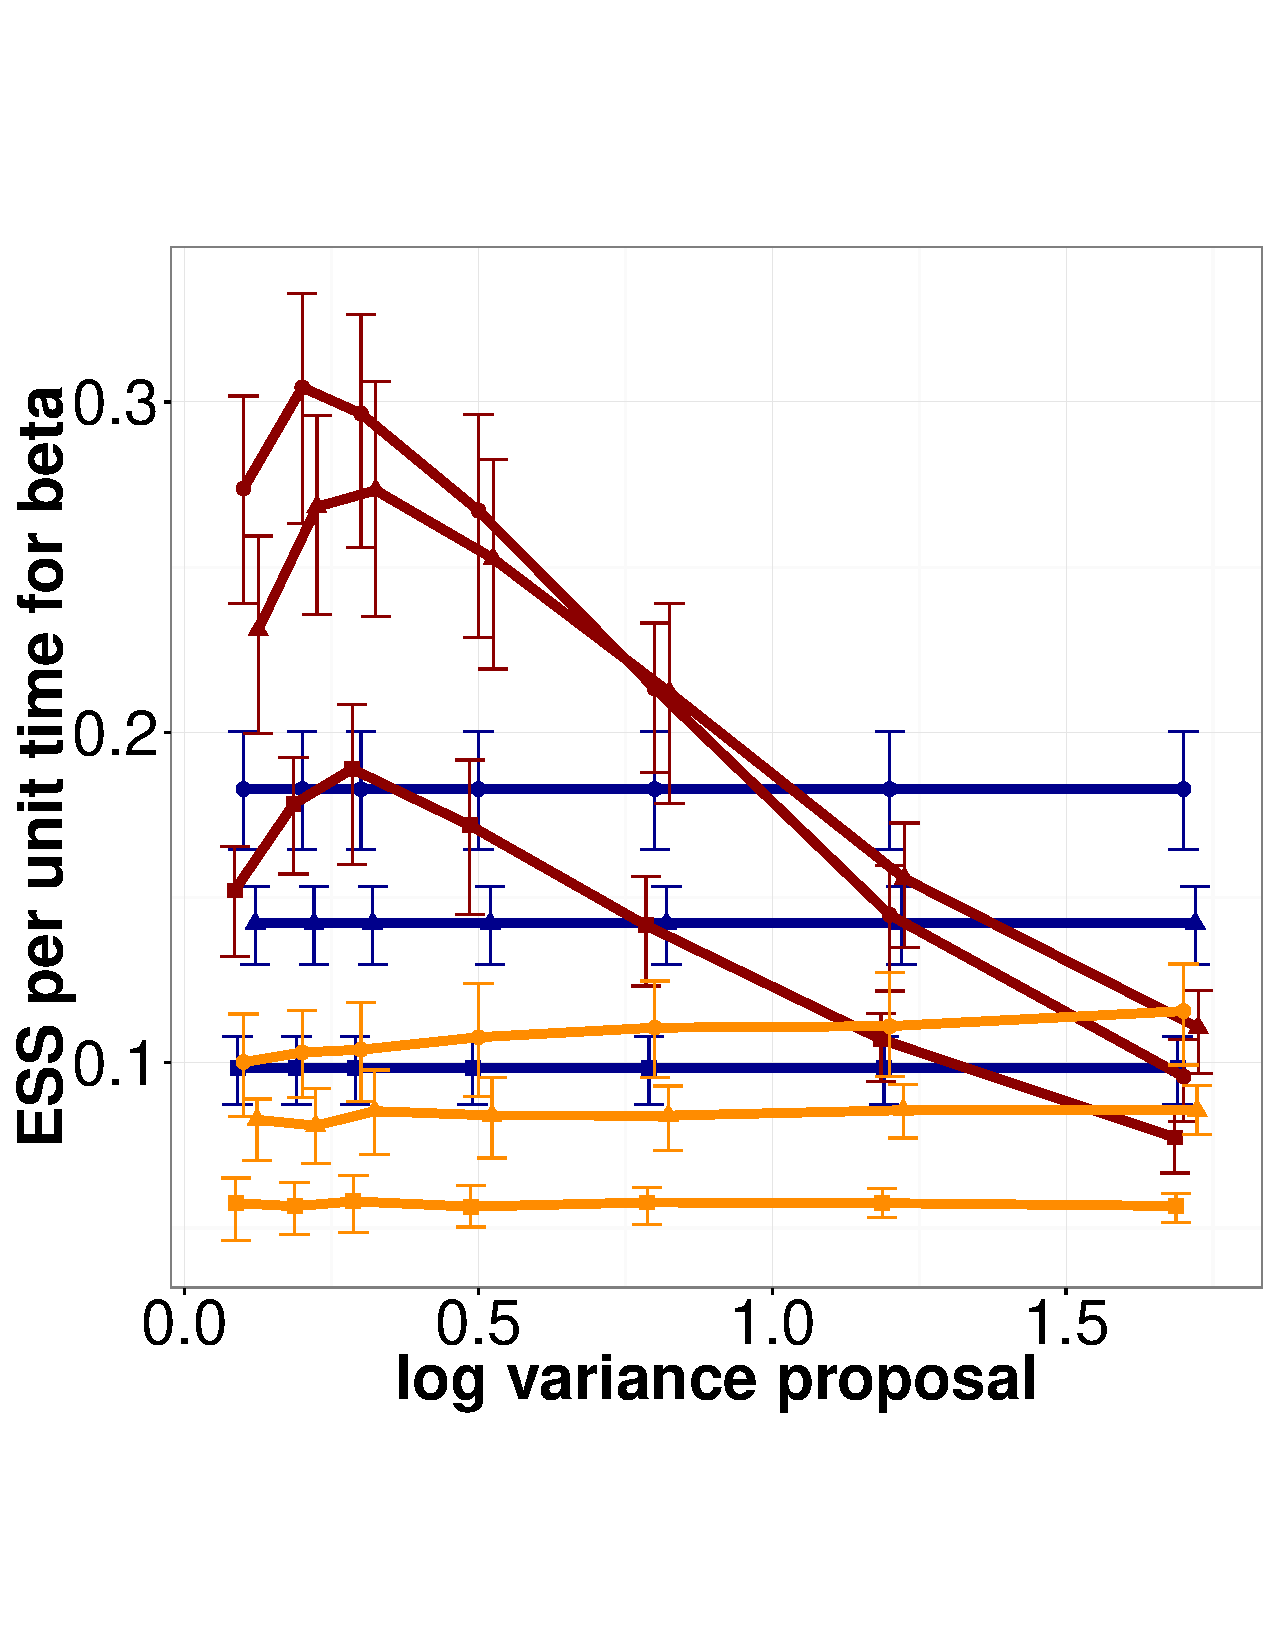
\includegraphics [width=0.70\textwidth, angle=0]{figs/pc_10_beta.pdf}
    \vspace{-0 in}
  \end{minipage}
     \label{fig:ESS_pc_10}
    \caption{ESS/sec for NH Immigration model (dim 10)}
  \end{figure}
